
\chapter{Introducción}
\label{sec:intro}


En este capitulo se presenta la motivación del proyecto, sus objetivos principales y la planificación general


\section{Motivación}


El presente Trabajo de Fin de Grado se enmarca en la creciente necesidad del sector inmobiliario de optimizar y modernizar sus procesos de gestión de propiedades y clientes. En un mercado cada vez más dinámico y competitivo, las herramientas tradicionales a menudo presentan limitaciones en términos de eficiencia, colaboración y acceso a la información en tiempo real.

La motivación principal de este proyecto surge de la identificación de estas deficiencias y de la oportunidad de aplicar tecnologías web modernas para crear una solución que impulse la productividad de los agentes inmobiliarios y mejore la experiencia del cliente. Específicamente, este TFG busca abordar los siguientes puntos clave:

\begin{enumerate}
    \item \textbf{Necesidad de Flexibilidad y Adaptabilidad en la Gestión de Datos:} Las bases de datos relacionales tradicionales, aunque robustas, a menudo imponen esquemas rígidos que dificultan la adaptación a los cambios constantes en las necesidades del negocio inmobiliario, como la inclusión de nuevos tipos de propiedades, atributos o métricas. Se observa una creciente tendencia hacia herramientas más ágiles en la gestión de datos.
    \item \textbf{Demanda de Colaboración y Acceso en Tiempo Real:} En el sector inmobiliario, la colaboración entre agentes, la actualización instantánea del estado de las propiedades y la programación de citas son vitales. Las soluciones existentes no siempre facilitan un entorno de trabajo colaborativo y accesible desde cualquier lugar.
    \item \textbf{Optimización de Procesos y Toma de Decisiones:} Los agentes inmobiliarios requieren de información clara y concisa para tomar decisiones estratégicas, como la valoración de propiedades o la identificación de inmuebles con baja rotación. La recopilación manual de datos o el uso de herramientas dispersas ralentiza este proceso.
\end{enumerate}

Para dar respuesta a estas motivaciones, se propone el desarrollo de la aplicación web \textbf{InmoTable}. Su justificación se basa en una serie de ventajas estratégicas y operativas:

\begin{itemize}
    \item \textbf{Eficiencia en el Desarrollo y Ahorro de Costes (Modelo \textit{No-Code/Low-Code}):} La utilización de una base de datos tipo spreadsheet como Airtable es una decisión fundamental que aporta una eficiencia significativa. Permite externalizar gran parte de la lógica de gestión de la empresa, reduciendo drásticamente la necesidad de programar módulos complejos de administración de datos en el backend y frontend. Esto se traduce en un ahorro considerable de tiempo y recursos de desarrollo y mantenimiento. La opción de un plan básico gratuito de Airtable y su escalabilidad a bajo coste en el futuro la convierten en una solución muy rentable desde el punto de vista económico. Además, su interfaz es altamente intuitiva y fácil de usar para los agentes inmobiliarios.
    \item \textbf{Flexibilidad y Adaptabilidad del Esquema de Datos:} A diferencia de las bases de datos tradicionales que requieren un esquema fijo, Airtable permite diseñar tablas y campos de forma dinámica, adaptándose rápidamente a las necesidades cambiantes del sector inmobiliario. Esta versatilidad es crucial cuando se manejan diferentes tipos de datos y se busca evitar las limitaciones de una estructura predefinida.
    \item \textbf{Colaboración en Tiempo Real y Acceso Remoto:} Airtable facilita que múltiples usuarios trabajen simultáneamente en los datos, con cambios instantáneos y accesibilidad remota, lo cual es esencial para equipos de agentes distribuidos o en constante movimiento.
    \item \textbf{Potencial de Automatización de Flujos de Trabajo:} La capacidad de crear flujos de trabajo automáticos directamente en Airtable (como el envío de notificaciones por email al agente al recibir un contacto o al cliente tras confirmar una cita) ahorra tiempo en tareas repetitivas y mejora la comunicación.
    \item \textbf{Modelo de Negocio Replicable (Franquiciable):} Una ventaja estratégica clave de esta arquitectura es su facilidad de replicación y adaptación para múltiples inmobiliarias. Una vez desarrollada la base de Airtable para una empresa, su implementación en una nueva inmobiliaria se simplifica enormemente: solo requeriría copiar la base de Airtable existente a un nuevo proyecto y actualizar las claves de API y nombres de configuración en el archivo environment de la aplicación web (Angular y Laravel). Esto transforma el proyecto en una solución "plug-and-play" para futuras implementaciones, lo que representa una propuesta de valor significativa para el mercado.
    \item \textbf{Experiencia de Usuario Diferenciada para el Cliente:} La implementación de un frontend en Angular ofrece una interfaz moderna, dinámica y atractiva para los clientes finales. Esto les permitirá buscar propiedades de manera eficiente, visualizar detalles completos y gestionar sus interacciones (como la programación de citas) de forma intuitiva, mejorando su experiencia general con la inmobiliaria.
    \item \textbf{Backend Robusto y Seguro con Laravel:} La capa de Laravel no solo facilita la comunicación entre Angular y Airtable, sino que también garantiza la seguridad y la fiabilidad del sistema mediante un control de autenticación y autorización (Laravel Passport), protegiendo la integridad de los datos y las operaciones.
    \item \textbf{Herramientas Analíticas Integradas para Agentes Inmobiliarios:} Mediante las interfaces y automatizaciones configuradas directamente en Airtable (Análisis de stock, Media de precios por tipo de inmueble, Visitas por propiedad, Tiempo medio de venta, Propiedades con baja rotación, entre otras), el proyecto empodera a los agentes con información valiosa para una toma de decisiones informada, mejorando la eficiencia operativa y la estrategia de ventas.
\end{itemize}

En síntesis, \textbf{InmoTable} no solo busca modernizar la gestión inmobiliaria a través de la digitalización, sino que también establece un modelo de trabajo dual innovador donde la flexibilidad y las capacidades de gestión de un sistema \textit{no-code/low-code} se combinan con la robustez y personalización de un desarrollo web a medida, creando una sinergia que beneficia tanto a los clientes como a los profesionales del sector.


\section{Objetivos}


El objetivo principal de este Trabajo de Fin de Grado es desarrollar una aplicación web de gestión inmobiliaria robusta, eficiente y escalable, que satisfaga las necesidades tanto de los clientes finales como de los agentes inmobiliarios, utilizando un enfoque híbrido que combine un desarrollo web a medida con las capacidades de una base de datos tipo spreadsheet.

Para alcanzar este objetivo general, se establecen los siguientes objetivos específicos:


\subsection{Objetivo principal}


Desarrollar una aplicación web integral para la gestión inmobiliaria, \textbf{InmoTable}, que proporcione una plataforma dual: una interfaz de usuario optimizada para clientes finales y un sistema de gestión y análisis de negocio eficiente para agentes inmobiliarios, logrando un equilibrio entre personalización y las ventajas de las herramientas \textit{no-code/low-code} \cite{ionos2024lowcode}.


\subsection{Objetivos específicos}


\begin{enumerate}
    \item \textbf{Diseñar y Desarrollar un Frontend Intuitivo para el Cliente:}
    \begin{itemize}
        \item Crear una interfaz de usuario atractiva y fácil de usar con Angular que permita a los clientes buscar, filtrar y visualizar propiedades de manera eficiente (listado y detalle).
        \item Implementar funcionalidades de autenticación y registro de usuarios para clientes, asegurando un acceso seguro y personalizado.
        \item Permitir a los clientes la interacción con la inmobiliaria mediante funcionalidades como la programación de citas para visitas y un formulario de contacto.
    \end{itemize}

    \item \textbf{Desarrollar un Backend Robusto y Seguro con Laravel:}
    \begin{itemize}
        \item Implementar una API RESTful en Laravel que actúe como una capa intermedia entre el frontend de Angular y la API de Airtable.
        \item Asegurar la comunicación y el acceso a los datos mediante la implementación de un sistema de autenticación y autorización basado en tokens con Laravel Passport.
        \item Gestionar las operaciones CRUD sobre las entidades (propiedades, clientes, agentes, citas) de forma segura y eficiente, traduciendo las solicitudes de la aplicación a interacciones con la API de Airtable.
    \end{itemize}

    \item \textbf{Implementar y Configurar Airtable como Plataforma de Gestión Central para Agentes:}
    \begin{itemize}
        \item Definir y estructurar las tablas de Airtable (Propiedades, Agentes, Clientes, Citas, Empresas, Usuarios, Contacto) para almacenar toda la información inmobiliaria de manera organizada y relacional.
        \item Configurar y personalizar las vistas de Airtable (ej. calendario de citas, galerías de propiedades, vistas de mapa) para facilitar a los agentes inmobiliarios la visualización y el seguimiento de los datos.
        \item Crear formularios de entrada de datos en Airtable para la fácil adición y modificación de registros por parte de los agentes (ej. Nueva Propiedad, Nueva Cita, Nuevo Cliente).
        \item Configurar automatizaciones en Airtable para gestionar flujos de trabajo clave, como el envío de notificaciones por correo electrónico a agentes y clientes, y la categorización automática de propiedades.
    \end{itemize}

    \item \textbf{Proveer Herramientas Analíticas y de Inteligencia de Negocio para Agentes (a través de Interfaces de Airtable):}
    Desarrollar dashboards interactivos en Airtable para ofrecer a los agentes una visión clara del rendimiento y estado del negocio. Esto incluye:
    \begin{itemize}
        \item Análisis de stock (métricas generales, propiedades disponibles, precio medio).
        \item Media de precios por tipo de inmueble (análisis de tendencias de mercado).
        \item Visitas por propiedad (seguimiento del interés en cada inmueble).
        \item Visitas programadas (gestión del calendario de citas).
        \item Tiempo medio de venta (análisis de eficiencia de rotación de propiedades).
        \item Propiedades con baja rotación (identificación de inmuebles que requieren atención).
        \item Propiedades (General) y Tipo de Propiedades (visión completa y categorizada del inventario).
    \end{itemize}

    \item \textbf{Demostrar la Viabilidad y Replicabilidad del Modelo de Negocio Híbrido:}

    \begin{itemize}
        \item Validar la eficiencia en el desarrollo y el ahorro de costes al aprovechar las funcionalidades \textit{no-code/low-code} de Airtable para la gestión interna de la empresa.
        \item Establecer la metodología de implementación del proyecto en nuevas inmobiliarias \cite{appmaster2024inmobiliarias}, demostrando la facilidad de replicación de la base de Airtable y la adaptación de la aplicación web mediante la configuración de variables de entorno.
    \end{itemize}

\end{enumerate}


\section{Planificación Temporal}


La planificación temporal de este Trabajo de Fin de Grado se estableció con una duración estimada inicial de 300 horas, distribuidas a lo largo de un curso académico. Esta estimación se basó en el alcance inicial del proyecto y en la complejidad de las tecnologías a integrar. Sin embargo, la implementación real del proyecto, en un ejercicio de transparencia y precisión, demandó un total de 395 horas, una cifra que, aunque supera la estimación inicial, se mantiene dentro de un rango justificado por la naturaleza innovadora y la profundización en las funcionalidades.

Esta sección detalla las fases clave del proyecto, la asignación de tiempo estimado y el tiempo real dedicado a cada una de sus sub-fases, proporcionando una base sólida para la creación de un cronograma visual detallado.

\textbf{Fases del Proyecto y Detalle Horario:}

\begin{enumerate}
    \item \textbf{Fase 1: Investigación y Diseño}
    \begin{itemize}
        \item \textbf{Horas Estimadas: 45 horas}
        \item \textbf{Horas Reales Invertidas: 55 horas}
        \begin{enumerate}
            \item \textbf{1.1. Definición de requisitos y alcance:} 15 horas estimadas / 20 horas reales. Esta sub-fase requirió una dedicación extra para una comprensión exhaustiva de las necesidades específicas de la gestión inmobiliaria para clientes y agentes, y para delinear cómo el enfoque híbrido (Angular/Laravel/Airtable) optimizaría estos procesos.
            \item \textbf{1.2. Análisis y selección de tecnologías principales:} 15 horas estimadas / 15 horas reales. La evaluación y justificación de la arquitectura se ajustó a lo previsto.
            \item \textbf{1.3. Diseño inicial de la estructura de datos en Airtable (tablas y relaciones):} 15 horas estimadas / 20 horas reales. La conceptualización y diseño inicial de las tablas de Airtable (Agentes, Citas, Clientes, Empresas, Propiedades, Usuarios, Contacto), considerando las relaciones y tipos de campos óptimos para una base de datos spreadsheet, demandó un poco más de tiempo.
        \end{enumerate}
    \end{itemize}
    \item \textbf{Fase 2: Desarrollo del Backend y Conexión con Airtable}
    \begin{itemize}
        \item \textbf{Horas Estimadas: 65 horas}
        \item \textbf{Horas Reales Invertidas: 70 horas}
        \begin{enumerate}
            \item \textbf{2.1. Implementación de la API RESTful en Laravel:} 20 horas estimadas / 25 horas reales. La creación de controladores y rutas que sirvieran como capa de abstracción para Airtable, incluyendo la validación y transformación de datos, requirió un esfuerzo adicional.
            \item \textbf{2.2. Desarrollo del AirtableService para interacción (CRUD):} 25 horas estimadas / 25 horas reales. La implementación de la lógica para interactuar con la API externa de Airtable, optimizando las llamadas y el manejo de respuestas, se gestionó dentro de lo previsto.
            \item \textbf{2.3. Configuración de autenticación (Laravel Passport):} 10 horas estimadas / 10 horas reales. La implementación del sistema de autenticación seguro basado en OAuth2 se mantuvo en línea con la estimación.
            \item \textbf{2.4. Configuración inicial de formularios y automatizaciones en Airtable (simples):} 10 horas estimadas / 10 horas reales. Creación de los primeros formularios (ej. Nueva Cita, Nueva Propiedad) y automatizaciones básicas para validar el flujo de datos.
        \end{enumerate}
    \end{itemize}
    \item \textbf{Fase 3: Desarrollo del Frontend (Aplicación Cliente)}
    \begin{itemize}
        \item \textbf{Horas Estimadas: 70 horas}
        \item \textbf{Horas Reales Invertidas: 80 horas}
        \begin{enumerate}
            \item \textbf{3.1. Implementación de componentes de interfaz de usuario (UI/UX) con Angular:} 45 horas estimadas / 55 horas reales. El desarrollo de interfaces para el cliente (listado y detalle de propiedades, formularios de citas y contacto, autenticación), con un fuerte enfoque en una experiencia de usuario fluida y un diseño receptivo, lo cual siempre consume más tiempo para asegurar la calidad.
            \item \textbf{3.2. Integración con servicios del backend de Laravel:} 20 horas estimadas / 20 horas reales. Conectar los componentes de Angular con los endpoints de la API de Laravel, manejando la comunicación asíncrona y la visualización correcta de los datos provenientes de Airtable.
            \item \textbf{3.3. Implementación de guardias de ruta y lógica de roles:} 5 horas estimadas / 5 horas reales. Asegurar que los diferentes perfiles de usuario accedan solo a las secciones correspondientes.
        \end{enumerate}
    \end{itemize}
    \item \textbf{Fase 4: Configuración y Personalización de Airtable (Herramienta para Agentes)}
    \begin{itemize}
        \item \textbf{Horas Estimadas: 30 horas}
        \item \textbf{Horas Reales Invertidas: 70 horas}
        \begin{enumerate}
            \item \textbf{4.1. Configuración avanzada de vistas de datos:} 10 horas estimadas / 20 horas reales. Diseño y optimización de las múltiples vistas de Airtable (calendario de citas, galerías, mapas, etc.) para ofrecer a los agentes herramientas de visualización de datos internas de alta calidad, lo cual fue un componente más extenso de lo previsto.
            \item \textbf{4.2. Desarrollo de interfaces analíticas (Dashboards) en Airtable:} 10 horas estimadas / 25 horas reales. La creación de los dashboards de análisis de negocio (Análisis de stock, Media de precios, Visitas por propiedad, Tiempo medio de venta, Propiedades con baja rotación, etc.) es un diferenciador clave que implicó una curva de aprendizaje y configuración más prolongada.
            \item \textbf{4.3. Optimización de formularios y automatizaciones de Airtable (avanzadas):} 10 horas estimadas / 25 horas reales. La creación y el ajuste fino de flujos de trabajo automatizados, incluyendo envíos de correos electrónicos condicionales y la gestión del ciclo de vida de las propiedades, representó un trabajo significativo en la plataforma Airtable.
        \end{enumerate}
    \end{itemize}
    \item \textbf{Fase 5: Pruebas, Despliegue, Ajustes y Documentación}
    \begin{itemize}
        \item \textbf{Horas Estimadas: 75 horas}
        \item \textbf{Horas Reales Invertidas: 110 horas}
        \begin{enumerate}
            \item \textbf{5.1. Realización de pruebas funcionales y de integración:} 15 horas estimadas / 20 horas reales. Verificación de la correcta funcionalidad e integración entre el frontend de Angular, el backend de Laravel y la API de Airtable, así como la gestión de la autenticación y la lógica de negocio, consumió más tiempo de depuración.
            \item \textbf{5.2. Despliegue y configuración del entorno (Docker):} 10 horas estimadas / 10 horas reales. Optimización de los contenedores Docker para producción y configuración de variables de entorno para la replicabilidad.
            \item \textbf{5.3. Redacción de la memoria del TFG y preparación de la defensa:} 50 horas estimadas / 80 horas reales. Esta es una de las fases más intensivas en cualquier TFG, implicando la estructuración, redacción detallada de la metodología, resultados, conclusiones, discusión de tecnologías, y la preparación exhaustiva de la presentación y su defensa, abarcando un rango significativo de horas en la realidad de este tipo de proyectos académicos. Se ha ajustado para reflejar este considerable esfuerzo intelectual y de síntesis.
        \end{enumerate}
    \end{itemize}
\end{enumerate}

\textbf{Tabla Resumen de Horas (para Cronograma Visual):}

\begin{figure}[H]
    \begin{center}
        \includegraphics[width = 0.95\textwidth]{Figuras/cronograma_tfg.png}
    \end{center}
    \caption{\label{fig:cronograma_tfg} Cronograma del TFG}
\end{figure}

\textbf{Justificación de la Desviación Temporal Global:}

La inversión total de 395 horas (frente a las 300 estimadas inicialmente) se justifica por la ambición y el nivel de detalle alcanzado en el proyecto, especialmente en áreas donde se maximizó el potencial de la plataforma Airtable y en la fase de documentación final. Las principales razones de esta extensión de tiempo son:
\begin{itemize}
    \item \textbf{Profundización en las Capacidades de Airtable como Plataforma de Negocio (Fase 4: +45 horas):} Esta fase experimentó una desviación significativa. La decisión de no solo usar Airtable como una base de datos, sino de explotar a fondo sus funcionalidades \textit{low-code} para crear interfaces analíticas avanzadas (dashboards de stock, precios, visitas, rotación) y automatizaciones complejas (envíos de emails, categorización de propiedades), requirió un tiempo de diseño, configuración y optimización significativamente mayor. Este esfuerzo es clave para la justificación del ahorro de desarrollo personalizado que ofrece el enfoque híbrido.
    \item \textbf{Complejidad de la Integración Híbrida (Fase 1, 2 y 3):} La interconexión fluida entre el frontend de Angular, el backend de Laravel y una API de terceros como Airtable implicó desafíos adicionales en la sincronización de datos, el manejo de errores y la optimización del rendimiento de las solicitudes API. Esto resultó en un ligero aumento acumulado en las fases de diseño y frontend (+10 y +10 horas respectivamente).
    \item \textbf{Redacción de la Memoria y Preparación de la Defensa (Fase 5.3: +65 horas):} La fase final de documentación y preparación de la defensa ha sido ajustada para reflejar un tiempo realista y sustancial (de 15 horas estimadas a 40 horas estimadas y de 40 horas reales a 65 horas reales para el total de la fase 5). La redacción de una memoria completa, que detalla la arquitectura, la implementación, los resultados y las reflexiones sobre la viabilidad del modelo de negocio, es un proceso intensivo que requiere múltiples revisiones y ajustes, justificando ampliamente el tiempo dedicado.
\end{itemize}
La inversión de estas horas adicionales ha permitido entregar una solución más completa, escalable y con un valor de negocio superior, validando la eficacia del enfoque híbrido propuesto para la gestión inmobiliaria digital.


\section{Resumen del documento}


El presente Trabajo de Fin de Grado describe el desarrollo de \textbf{InmoTable}, una aplicación web innovadora para la gestión inmobiliaria. La memoria se organiza de la siguiente manera:

\begin{itemize}
    \item \textbf{Capítulo ~\ref{sec:intro}. Introducción:} Presenta la motivación del proyecto, sus objetivos principales y la planificación general.

    \item \textbf{Capítulo ~\ref{sec:analisisviabilidad}. Análisis de viabilidad:} Evalúa la factibilidad técnica y económica de la solución, destacando su bajo coste y alta replicabilidad gracias al uso de Airtable.

    \item \textbf{Capítulo ~\ref{sec:modelosdesarrollotecnologias}. Modelos de desarrollo y tecnologías:} Detalla la metodología Scrum empleada y justifica la elección de Angular, Laravel y Airtable frente a otras opciones.

    \item \textbf{Capítulo ~\ref{sec:inmotable}. InmoTable:} Describe en profundidad el diseño y la implementación del sistema, abarcando su arquitectura, el modelo de datos y las interfaces de usuario para clientes (web) y agentes (Airtable).

    \item \textbf{Capítulo ~\ref{sec:conclusionesytrabajosfuturos}. Conclusiones y trabajos futuros:} Recoge los resultados clave del proyecto y propone futuras líneas de evolución.

    \item \textbf{Capítulo 6. Bibliografía:} Contiene todas las referencias documentales utilizadas.
\end{itemize}


\chapter{Análisis de viabilidad} 
\label{sec:analisisviabilidad}


En este capitulo se evalúa la factibilidad técnica y económica de la solución, destacando su bajo coste y alta replicabilidad gracias al uso de Airtable.


\section{Situación actual}


La concepción del proyecto \textbf{InmoTable} surge de un análisis del mercado actual de soluciones de gestión inmobiliaria, donde se ha identificado una oportunidad significativa para ofrecer una alternativa que combine la eficiencia del desarrollo web con la agilidad de las plataformas \textit{low-code}. La motivación principal para realizar este proyecto se basa en los siguientes pilares de diferenciación:

\begin{itemize}
    \item \textbf{Identificación de un Nicho de Mercado:} Se ha detectado una carencia de soluciones en el mercado que ofrezcan una aplicación web intuitiva y moderna para el cliente final, al mismo tiempo que proporcionan una plataforma de gestión interna (CRM/ERP) excepcionalmente flexible, de bajo coste y fácil de usar para los agentes inmobiliarios, sin la necesidad de un desarrollo a medida complejo para la administración del día a día. Las soluciones existentes suelen ser o bien CRMs robustos y costosos que requieren una alta inversión inicial y personalización, o bien herramientas muy simples que no escalan.
    \item \textbf{Eficiencia en el Desarrollo y Sencillez de Implementación:} El enfoque híbrido adoptado, que delega la mayor parte de la lógica de gestión interna a Airtable, convierte el proceso de desarrollo personalizado del backend y el frontend en algo notablemente más sencillo y rápido de programar. Al no tener que construir desde cero complejos paneles de administración, formularios dinámicos, módulos de análisis de datos o sistemas de automatización de flujos de trabajo (que ya están preconstruidos y son altamente configurables en Airtable), se logra una reducción drástica en el tiempo y el esfuerzo de ingeniería.
    \item \textbf{Minimización de Costes Operativos y de Licencia:} La elección de Airtable es fundamental desde el punto de vista económico. Al disponer de una opción básica gratuita y planes de pago muy asequibles y escalables, se reduce significativamente la barrera de entrada para las inmobiliarias, eliminando la necesidad de adquirir licencias costosas de software de gestión o de invertir en infraestructura de bases de datos tradicional. Esto no solo abarata el coste de adquisición, sino también el de operación y mantenimiento.
    \item \textbf{Alta Portabilidad y Replicabilidad del Modelo de Negocio:} Una de las ventajas más estratégicas de \textbf{InmoTable} es su inherente portabilidad. Una vez desarrollada y optimizada la base de Airtable para una inmobiliaria, el modelo puede ser replicado y adaptado a una nueva agencia de forma extremadamente rápida, simplemente clonando la base de Airtable y ajustando unas pocas variables de entorno (claves de API, nombres de base) en la aplicación web (Angular y Laravel). Esto hace que la solución sea altamente "franquiciable" y atractiva para el mercado, permitiendo una expansión rápida y de bajo coste.
\end{itemize}

\section{Ingeniería de Requisitos}


Durante esta fase se ha realizado un análisis detallado para identificar las necesidades que debe cubrir el sistema. Esta definición de requisitos constituye la base sobre la cual se diseñará y desarrollará la aplicación. Para organizar esta información, se han clasificado los requisitos en tres apartados principales:

\begin{itemize}
    \item \textbf{Actores:} Los actores son todas aquellas entidades (personas o sistemas) que interactúan con el sistema.
    \item \textbf{Requisitos funcionales:} Son las funcionalidades que debe ofrecer el sistema para satisfacer las necesidades de los usuarios dentro del dominio inmobiliario.
    \item \textbf{Requisitos no funcionales:} Son las condiciones que debe cumplir el sistema respecto al entorno, calidad y restricciones de uso.
\end{itemize}


% ACTORES
\subsection{Actores}


\begin{table}[H]
\centering
\begin{tabular}{|p{3cm}|p{10cm}|}
\hline
\rowcolor{tealblue}
{\textbf{ACT-01}} & {\textbf{Sin Usuario (Web App)}} \\
\hline
Descripción & Usuario anónimo que navega por la aplicación web sin autenticarse, puede ver propiedades públicas y solicitar atención mediante contacto. \\
\hline
Comentarios & No dispondrá de acceso a funcionalidades que requieren autenticación. \\
\hline
\end{tabular}
\caption{Actor ACT-01: Sin Usuario (Web App)}
\end{table}

\begin{table}[H]
\centering
\begin{tabular}{|p{3cm}|p{10cm}|}
\hline
\rowcolor{tealblue}
{\textbf{ACT-02}} & {\textbf{Cliente (Web App)}} \\
\hline
Descripción & Usuario registrado y autenticado en la aplicación web con acceso a funcionalidades personalizadas como gestión de intereses, solicitar y visualizar citar, y modificar perfil. \\
\hline
Comentarios & Requiere registro y autenticación para acceder a funcionalidades completas. \\
\hline
\end{tabular}
\caption{Actor ACT-02: Cliente (Web App)}
\end{table}

\begin{table}[H]
\centering
\begin{tabular}{|p{3cm}|p{10cm}|}
\hline
\rowcolor{tealblue}
{\textbf{ACT-03}} & {\textbf{Agente (AirTable)}} \\
\hline
Descripción & Usuario con funciones operacionales, gestiona propiedades, clientes y citas desde AirTable con permisos de edición limitados. \\
\hline
Comentarios & Acceso exclusivo a través de AirTable, sin acceso directo a la aplicación web. \\
\hline
\end{tabular}
\caption{Actor ACT-03: Agente (AirTable)}
\end{table}

\begin{table}[H]
\centering
\begin{tabular}{|p{3cm}|p{10cm}|}
\hline
\rowcolor{tealblue}
{\textbf{ACT-04}} & {\textbf{Administrador (AirTable)}} \\
\hline
Descripción & Usuario con funciones de administrador, control total sobre el sistema incluyendo gestión de usuarios, configuración de empresa y eliminación de datos. \\
\hline
Comentarios & Permisos completos en AirTable para gestión y configuración del sistema. \\
\hline
\end{tabular}
\caption{Actor ACT-04: Administrador (AirTable)}
\end{table}


% REQUISITOS FUNCIONALES
\subsection{Requisitos Funcionales}


% Requisitos Funcionales de la Aplicación Web (Frontend para Clientes)
\subsubsection{Requisitos Funcionales de la Aplicación Web}


\begin{table}[H]
\centering
\begin{tabular}{|p{3cm}|p{10cm}|}
\hline
\rowcolor{tealblue}
\textbf{RF 01.1} & \textbf{Buscar Propiedades por Criterios} \\
\hline
\textbf{Actores} & ACT-01, ACT-02 \\
\hline
\textbf{Descripción} & Permite al usuario (visitante o cliente registrado) buscar propiedades utilizando filtros como precio, tipo de propiedad, número de habitaciones, etc., para refinar los resultados de su interés. \\
\hline
\textbf{Precondiciones} & Acceso a la aplicación web. \\
\hline
\end{tabular}
\caption{RF 01.1: Buscar Propiedades por Criterios}
\end{table}

\begin{table}[H]
\centering
\begin{tabular}{|p{3cm}|p{10cm}|}
\hline
\rowcolor{tealblue}
\textbf{RF 01.2} & \textbf{Visualizar Listado de Propiedades} \\
\hline
\textbf{Actores} & ACT-01, ACT-02 \\
\hline
\textbf{Descripción} & Muestra una lista paginada de propiedades disponibles, presentando información básica como la imagen principal, la referencia y el precio. \\
\hline
\textbf{Precondiciones} & Acceso a la aplicación web. \\
\hline
\end{tabular}
\caption{RF 01.2: Visualizar Listado de Propiedades}
\end{table}

\begin{table}[H]
\centering
\begin{tabular}{|p{3cm}|p{10cm}|}
\hline
\rowcolor{tealblue}
\textbf{RF 01.3} & \textbf{Visualizar Detalle de Propiedad} \\
\hline
\textbf{Actores} & ACT-01, ACT-02 \\
\hline
\textbf{Descripción} & Permite acceder a una página dedicada con toda la información detallada de una propiedad, incluyendo fotos adicionales, descripción completa y características específicas. \\
\hline
\textbf{Precondiciones} & Acceso a la aplicación web; Propiedad seleccionada del listado. \\
\hline
\end{tabular}
\caption{RF 01.3: Visualizar Detalle de Propiedad}
\end{table}

\begin{table}[H]
\centering
\begin{tabular}{|p{3cm}|p{10cm}|}
\hline
\rowcolor{tealblue}
\textbf{RF 01.4} & \textbf{Registrarse como Cliente} \\
\hline
\textbf{Actores} & ACT-01, ACT-02 \\
\hline
\textbf{Descripción} & Permite a nuevos usuarios crear una cuenta de cliente en la aplicación web para acceder a funcionalidades personalizadas y guardar preferencias. \\
\hline
\textbf{Precondiciones} & Acceso a la aplicación web; Usuario no autenticado. \\
\hline
\end{tabular}
\caption{RF 01.4: Registrarse como Cliente}
\end{table}

\begin{table}[H]
\centering
\begin{tabular}{|p{3cm}|p{10cm}|}
\hline
\rowcolor{tealblue}
\textbf{RF 01.5} & \textbf{Iniciar Sesión (Cliente)} \\
\hline
\textbf{Actores} & ACT-01, ACT-02 \\
\hline
\textbf{Descripción} & Permite a los clientes registrados autenticarse en el sistema utilizando sus credenciales (email y contraseña). \\
\hline
\textbf{Precondiciones} & Acceso a la aplicación web; Cuenta de cliente existente; Usuario no autenticado. \\
\hline
\end{tabular}
\caption{RF 01.5: Iniciar Sesión (Cliente)}
\end{table}

\begin{table}[H]
\centering
\begin{tabular}{|p{3cm}|p{10cm}|}
\hline
\rowcolor{tealblue}
\textbf{RF 01.6} & \textbf{Enviar Mensaje de Contacto} \\
\hline
\textbf{Actores} & ACT-01, ACT-02 \\
\hline
\textbf{Descripción} & Permite a cualquier usuario (visitante o cliente registrado) enviar una consulta general o un mensaje a la inmobiliaria a través de un formulario web. \\
\hline
\textbf{Precondiciones} & Acceso a la aplicación web. \\
\hline
\end{tabular}
\caption{RF 01.6: Enviar Mensaje de Contacto}
\end{table}

\begin{table}[H]
\centering
\begin{tabular}{|p{3cm}|p{10cm}|}
\hline
\rowcolor{tealblue}
\textbf{RF 01.7} & \textbf{Solicitar Cita para Propiedad} \\
\hline
\textbf{Actores} & ACT-02 \\
\hline
\textbf{Descripción} & Permite a un cliente registrado programar una visita para una propiedad específica, indicando la fecha y hora preferidas. La solicitud será enviada a Airtable para su gestión por el agente. \\
\hline
\textbf{Precondiciones} & Cliente autenticado (sesión iniciada); Propiedad existente y disponible para citas. \\
\hline
\end{tabular}
\caption{RF 01.7: Solicitar Cita para Propiedad}
\end{table}


% Requisitos Funcionales del Sistema de Gestión Interna (Airtable para Agentes/Administradores)
\subsubsection{Requisitos Funcionales del Sistema de Gestión Interna (Airtable)}

\begin{table}[H]
    \centering
    \begin{tabular}{|p{3cm}|p{10cm}|}
    \hline
        \rowcolor{tealblue}
        \textbf{RF 02.1} & \textbf{Crear Nueva Propiedad} \\
    \hline
        \textbf{Actores} & ACT-03, ACT-04 \\
    \hline
        \textbf{Descripción} & Permitir a los agentes y administradores añadir nuevos inmuebles al inventario utilizando los formularios personalizados de Airtable, incluyendo todos los detalles de la propiedad y la carga de fotos. \\
    \hline
        \textbf{Precondiciones} & Acceso a Airtable con rol ACT-03 o ACT-04. \\
    \hline
    \end{tabular}
        \caption{RF 02.1: Crear Nueva Propiedad}
        \label{tab:rf_airtable_2_1}
\end{table}

\begin{table}[H]
\centering
\begin{tabular}{|p{3cm}|p{10cm}|}
\hline
\rowcolor{tealblue}
\textbf{RF 02.2} & \textbf{Consultar Propiedades (en Airtable)} \\
\hline
\textbf{Actores} & ACT-03, ACT-04 \\
\hline
\textbf{Descripción} & Permitir a los agentes y administradores visualizar la información detallada de las propiedades en diversas vistas personalizadas de Airtable (grid, galería de fotos, vista de mapa, etc.). \\
\hline
\textbf{Precondiciones} & Acceso a Airtable con rol ACT-03 o ACT-04. \\
\hline
\end{tabular}
\caption{RF 02.2: Consultar Propiedades (en Airtable)}
\label{tab:rf_airtable_2_2}
\end{table}

\begin{table}[H]
\centering
\begin{tabular}{|p{3cm}|p{10cm}|}
\hline
\rowcolor{tealblue}
\textbf{RF 02.3} & \textbf{Actualizar Información de Propiedad} \\
\hline
\textbf{Actores} & ACT-03, ACT-04 \\
\hline
\textbf{Descripción} & Permitir a los agentes y administradores modificar los datos existentes de las propiedades en Airtable, incluyendo cambios de precio, estado, descripción o características. \\
\hline
\textbf{Precondiciones} & Acceso a Airtable con rol ACT-03 o ACT-04; Propiedad existente. \\
\hline
\end{tabular}
\caption{RF 02.3: Actualizar Información de Propiedad}
\label{tab:rf_airtable_2_3}
\end{table}

\begin{table}[H]
\centering
\begin{tabular}{|p{3cm}|p{10cm}|}
\hline
\rowcolor{tealblue}
\textbf{RF 02.4} & \textbf{Eliminar Propiedad} \\
\hline
\textbf{Actores} & ACT-03, ACT-04 \\
\hline
\textbf{Descripción} & Permitir a los agentes y administradores dar de baja o eliminar propiedades del inventario en Airtable. \\
\hline
\textbf{Precondiciones} & Acceso a Airtable con rol ACT-03 o ACT-04; Propiedad existente. \\
\hline
\end{tabular}
\caption{RF 02.4: Eliminar Propiedad}
\label{tab:rf_airtable_2_4}
\end{table}

\begin{table}[H]
\centering
\begin{tabular}{|p{3cm}|p{10cm}|}
\hline
\rowcolor{tealblue}
\textbf{RF 03.1} & \textbf{Programar y Modificar Citas} \\
\hline
\textbf{Actores} & ACT-03, ACT-04 \\
\hline
\textbf{Descripción} & Permitir a los agentes y administradores crear nuevas citas para los clientes o ajustar los detalles de citas ya programadas en Airtable, incluyendo fecha, hora, cliente y propiedad asociada. \\
\hline
\textbf{Precondiciones} & Acceso a Airtable con rol ACT-03 o ACT-04; Cliente y/o Propiedad existente. \\
\hline
\end{tabular}
\caption{RF 03.1: Programar y Modificar Citas}
\label{tab:rf_airtable_3_1}
\end{table}

\begin{table}[H]
\centering
\begin{tabular}{|p{3cm}|p{10cm}|}
\hline
\rowcolor{tealblue}
\textbf{RF 03.2} & \textbf{Visualizar Calendario de Citas} \\
\hline
\textbf{Actores} & ACT-03, ACT-04 \\
\hline
\textbf{Descripción} & Permitir a los agentes y administradores consultar la agenda de citas programadas en un formato de calendario interactivo dentro de Airtable, facilitando la planificación y seguimiento diario. \\
\hline
\textbf{Precondiciones} & Acceso a Airtable con rol ACT-03 o ACT-04. \\
\hline
\end{tabular}
\caption{RF 03.2: Visualizar Calendario de Citas}
\label{tab:rf_airtable_3_2}
\end{table}

\begin{table}[H]
\centering
\begin{tabular}{|p{3cm}|p{10cm}|}
\hline
\rowcolor{tealblue}
\textbf{RF 03.3} & \textbf{Actualizar Estado de Cita} \\
\hline
\textbf{Actores} & ACT-03, ACT-04 \\
\hline
\textbf{Descripción} & Permitir a los agentes y administradores cambiar el estado de una cita (ej., de "Pendiente" a "Confirmada", "Realizada" o "Cancelada") en Airtable, reflejando el progreso de la interacción con el cliente. \\
\hline
\textbf{Precondiciones} & Acceso a Airtable con rol ACT-03 o ACT-04; Cita existente. \\
\hline
\end{tabular}
\caption{RF 03.3: Actualizar Estado de Cita}
\label{tab:rf_airtable_3_3}
\end{table}

\begin{table}[H]
\centering
\begin{tabular}{|p{3cm}|p{10cm}|}
\hline
\rowcolor{tealblue}
\textbf{RF 04.1} & \textbf{Registrar Nuevo Cliente} \\
\hline
\textbf{Actores} & ACT-03, ACT-04 \\
\hline
\textbf{Descripción} & Permitir a los agentes y administradores registrar la información de nuevos clientes en la base de datos de Airtable a través de formularios, incluyendo datos de contacto y preferencias iniciales. \\
\hline
\textbf{Precondiciones} & Acceso a Airtable con rol ACT-03 o ACT-04. \\
\hline
\end{tabular}
\caption{RF 04.1: Registrar Nuevo Cliente}
\label{tab:rf_airtable_4_1}
\end{table}

\begin{table}[H]
\centering
\begin{tabular}{|p{3cm}|p{10cm}|}
\hline
\rowcolor{tealblue}
\textbf{RF 04.2} & \textbf{Consultar y Actualizar Cliente} \\
\hline
\textbf{Actores} & ACT-03, ACT-04 \\
\hline
\textbf{Descripción} & Permitir a los agentes y administradores acceder y modificar los detalles de los clientes existentes en Airtable, incluyendo sus preferencias de vivienda y el historial de interacciones. \\
\hline
\textbf{Precondiciones} & Acceso a Airtable con rol ACT-03 o ACT-04; Cliente existente. \\
\hline
\end{tabular}
\caption{RF 04.2: Consultar y Actualizar Cliente}
\label{tab:rf_airtable_4_2}
\end{table}

\begin{table}[H]
\centering
\begin{tabular}{|p{3cm}|p{10cm}|}
\hline
\rowcolor{tealblue}
\textbf{RF 05.1} & \textbf{Visualizar Análisis de Stock} \\
\hline
\textbf{Actores} & ACT-03, ACT-04 \\
\hline
\textbf{Descripción} & Proporcionar a los agentes y administradores acceso a dashboards visuales en Airtable con métricas generales del inventario de propiedades (total, disponibles, precio medio, superficie media, propiedades por tipo y estado) para una visión ejecutiva del negocio. \\
\hline
\textbf{Precondiciones} & Acceso a Airtable con rol ACT-03 o ACT-04. \\
\hline
\end{tabular}
\caption{RF 05.1: Visualizar Análisis de Stock}
\label{tab:rf_airtable_5_1}
\end{table}

\begin{table}[H]
\centering
\begin{tabular}{|p{3cm}|p{10cm}|}
\hline
\rowcolor{tealblue}
\textbf{RF 05.2} & \textbf{Visualizar Media de Precios por Tipo de Inmueble} \\
\hline
\textbf{Actores} & ACT-03, ACT-04 \\
\hline
\textbf{Descripción} & Permitir el acceso a gráficos y métricas que muestran el valor promedio de las propiedades desglosado por su tipo (ej. apartamentos, casas, oficinas), facilitando el análisis de tendencias de mercado. \\
\hline
\textbf{Precondiciones} & Acceso a Airtable con rol ACT-03 o ACT-04. \\
\hline
\end{tabular}
\caption{RF 05.2: Visualizar Media de Precios por Tipo de Inmueble}
\label{tab:rf_airtable_5_2}
\end{table}

\begin{table}[H]
\centering
\begin{tabular}{|p{3cm}|p{10cm}|}
\hline
\rowcolor{tealblue}
\textbf{RF 05.3} & \textbf{Visualizar Visitas por Propiedad} \\
\hline
\textbf{Actores} & ACT-03, ACT-04 \\
\hline
\textbf{Descripción} & Permitir a los usuarios monitorear el número de citas (visitas) asociadas a cada propiedad, incluyendo un detalle de las mismas, para evaluar el interés y la demanda de inmuebles. \\
\hline
\textbf{Precondiciones} & Acceso a Airtable con rol ACT-03 o ACT-04. \\
\hline
\end{tabular}
\caption{RF 05.3: Visualizar Visitas por Propiedad}
\label{tab:rf_airtable_5_3}
\end{table}

\begin{table}[H]
\centering
\begin{tabular}{|p{3cm}|p{10cm}|}
\hline
\rowcolor{tealblue}
\textbf{RF 05.4} & \textbf{Visualizar Tiempo Medio de Venta/Rotación} \\
\hline
\textbf{Actores} & ACT-03, ACT-04 \\
\hline
\textbf{Descripción} & Proporcionar acceso a datos y métricas que informan sobre el tiempo promedio que una propiedad permanece en el mercado hasta su venta o alquiler, desglosado por tipo de inmueble, para evaluar la eficiencia operativa. \\
\hline
\textbf{Precondiciones} & Acceso a Airtable con rol ACT-03 o ACT-04. \\
\hline
\end{tabular}
\caption{RF 05.4: Visualizar Tiempo Medio de Venta/Rotación}
\label{tab:rf_airtable_5_4}
\end{table}

\begin{table}[H]
\centering
\begin{tabular}{|p{3cm}|p{10cm}|}
\hline
\rowcolor{tealblue}
\textbf{RF 05.5} & \textbf{Visualizar Propiedades con Baja Rotación} \\
\hline
\textbf{Actores} & ACT-03, ACT-04 \\
\hline
\textbf{Descripción} & Identificar y listar las propiedades que han permanecido en el inventario por un período de tiempo superior a un umbral definido, mostrando sus detalles y días en el mercado para una gestión proactiva. \\
\hline
\textbf{Precondiciones} & Acceso a Airtable con rol ACT-03 o ACT-04. \\
\hline
\end{tabular}
\caption{RF 05.5: Visualizar Propiedades con Baja Rotación}
\label{tab:rf_airtable_5_5}
\end{table}

\begin{table}[H]
\centering
\begin{tabular}{|p{3cm}|p{10cm}|}
\hline
\rowcolor{tealblue}
\textbf{RF 05.6} & \textbf{Visualizar Distribución por Tipo de Propiedad} \\
\hline
\textbf{Actores} & ACT-03, ACT-04 \\
\hline
\textbf{Descripción} & Entender la composición del inventario de propiedades mediante gráficos que muestran la cantidad de inmuebles por cada tipo (ej. apartamentos, casas, chalets), ayudando a la estrategia de negocio. \\
\hline
\textbf{Precondiciones} & Acceso a Airtable con rol ACT-03 o ACT-04. \\
\hline
\end{tabular}
\caption{RF 05.6: Visualizar Distribución por Tipo de Propiedad}
\label{tab:rf_airtable_5_6}
\end{table}

\begin{table}[H]
\centering
\begin{tabular}{|p{3cm}|p{10cm}|}
\hline
\rowcolor{tealblue}
\textbf{RF 06.1} & \textbf{Administrar Usuarios Internos y Roles} \\
\hline
\textbf{Actores} & ACT-04 \\
\hline
\textbf{Descripción} & Permitir al administrador crear, modificar y eliminar registros de agentes o administradores directamente en Airtable, y asignar o ajustar sus roles de acceso para gestionar el personal interno. \\
\hline
\textbf{Precondiciones} & Acceso a Airtable con rol ACT-04. \\
\hline
\end{tabular}
\caption{RF 06.1: Administrar Usuarios Internos y Roles}
\label{tab:rf_airtable_6_1}
\end{table}

\begin{table}[H]
\centering
\begin{tabular}{|p{3cm}|p{10cm}|}
\hline
\rowcolor{tealblue}
\textbf{RF 06.2} & \textbf{Configurar y Supervisar Automatizaciones} \\
\hline
\textbf{Actores} & ACT-03, ACT-04 \\
\hline
\textbf{Descripción} & Permitir a los usuarios internos ajustar las reglas de automatización en Airtable (ej., envío de notificaciones por email al agente al recibir un contacto o al cliente tras confirmar una cita) y monitorear su ejecución para optimizar flujos de trabajo. \\
\hline
\textbf{Precondiciones} & Acceso a Airtable con rol ACT-03 o ACT-04. \\
\hline
\end{tabular}
\caption{RF 06.2: Configurar y Supervisar Automatizaciones}
\label{tab:rf_airtable_6_2}
\end{table}

\begin{table}[H]
\centering
\begin{tabular}{|p{3cm}|p{10cm}|}
\hline
\rowcolor{tealblue}
\textbf{RF 06.3} & \textbf{Personalizar Vistas y Formularios (Airtable)} \\
\hline
\textbf{Actores} & ACT-04 \\
\hline
\textbf{Descripción} & Permitir al administrador diseñar y ajustar las vistas de datos (grid, calendario, galería, mapa) y los formularios de entrada de datos en Airtable para optimizar la visualización y gestión operativa del equipo. \\
\hline
\textbf{Precondiciones} & Acceso a Airtable con rol ACT-04. \\
\hline
\end{tabular}
\caption{RF 06.3: Personalizar Vistas y Formularios (Airtable)}
\label{tab:rf_airtable_6_3}
\end{table}


% REQUISITOS NO FUNCIONALES
\subsection{Requisitos No Funcionales}


% RNF-01: RENDIMIENTO

\begin{table}[H]
\centering
\begin{tabular}{|p{3cm}|p{10cm}|}
\hline
\rowcolor{tealblue}
{\textbf{RNF-01.1}} & {\textbf{Tiempo de Carga de Páginas}} \\
\hline
Tipo de requisito & No Funcional - Rendimiento \\
\hline
Descripción & Las páginas de la aplicación web deben cargar en menos de 3 segundos con conexión estándar de banda ancha. \\
\hline
Criterio de Aceptación & Tiempo de carga $\leq$ 3 segundos medido con herramientas como Lighthouse \\
\hline
\end{tabular}
\caption{Requisito RNF-01.1}
\end{table}

\begin{table}[H]
\centering
\begin{tabular}{|p{3cm}|p{10cm}|}
\hline
\rowcolor{tealblue}
{\textbf{RNF-01.2}} & {\textbf{Sincronización con AirTable}} \\
\hline
Tipo de requisito & No Funcional - Rendimiento \\
\hline
Descripción & Los cambios realizados en AirTable deben reflejarse en la aplicación web en un tiempo máximo de 5 minutos. \\
\hline
Criterio de Aceptación & Latencia de sincronización $\leq$ 5 minutos para cualquier cambio en AirTable \\
\hline
\end{tabular}
\caption{Requisito RNF-01.2}
\end{table}

\begin{table}[H]
\centering
\begin{tabular}{|p{3cm}|p{10cm}|}
\hline
\rowcolor{tealblue}
{\textbf{RNF-01.3}} & {\textbf{Optimización de Imágenes}} \\
\hline
Tipo de requisito & No Funcional - Rendimiento \\
\hline
Descripción & Las imágenes de propiedades deben optimizarse automáticamente con lazy loading y compresión para mejorar tiempos de carga. \\
\hline
Criterio de Aceptación & Imágenes con compresión automática y carga diferida implementada \\
\hline
\end{tabular}
\caption{Requisito RNF-01.3}
\end{table}

% RNF-02: USABILIDAD

\begin{table}[H]
\centering
\begin{tabular}{|p{3cm}|p{10cm}|}
\hline
\rowcolor{tealblue}
{\textbf{RNF-02.1}} & {\textbf{Diseño Responsive}} \\
\hline
Tipo de requisito & No Funcional - Usabilidad \\
\hline
Descripción & La aplicación debe ser completamente funcional y visualmente correcta en dispositivos móviles, tabletas y escritorio. \\
\hline
Criterio de Aceptación & Compatibilidad verificada en resoluciones desde 320px hasta 1920px \\
\hline
\end{tabular}
\caption{Requisito RNF-02.1}
\end{table}

\begin{table}[H]
\centering
\begin{tabular}{|p{3cm}|p{10cm}|}
\hline
\rowcolor{tealblue}
{\textbf{RNF-02.2}} & {\textbf{Interfaz Intuitiva}} \\
\hline
Tipo de requisito & No Funcional - Usabilidad \\
\hline
Descripción & La navegación debe ser intuitiva permitiendo que un usuario nuevo pueda realizar tareas básicas sin entrenamiento previo. \\
\hline
Criterio de Aceptación & Máximo 3 clics para acceder a cualquier funcionalidad principal \\
\hline
\end{tabular}
\caption{Requisito RNF-02.2}
\end{table}

\begin{table}[H]
\centering
\begin{tabular}{|p{3cm}|p{10cm}|}
\hline
\rowcolor{tealblue}
{\textbf{RNF-02.3}} & {\textbf{Accesibilidad Web}} \\
\hline
Tipo de requisito & No Funcional - Usabilidad \\
\hline
Descripción & La aplicación debe cumplir con estándares WCAG 2.1 nivel AA para garantizar accesibilidad a usuarios con discapacidades. \\
\hline
Criterio de Aceptación & Cumplimiento verificado con herramientas de auditoría de accesibilidad \\
\hline
\end{tabular}
\caption{Requisito RNF-02.3}
\end{table}

% RNF-03: COMPATIBILIDAD

\begin{table}[H]
\centering
\begin{tabular}{|p{3cm}|p{10cm}|}
\hline
\rowcolor{tealblue}
{\textbf{RNF-03.1}} & {\textbf{Compatibilidad de Navegadores}} \\
\hline
Tipo de requisito & No Funcional - Compatibilidad \\
\hline
Descripción & La aplicación debe funcionar correctamente en las últimas 2 versiones de Chrome, Firefox, Safari y Edge. \\
\hline
Criterio de Aceptación & Funcionalidad completa verificada en navegadores especificados \\
\hline
\end{tabular}
\caption{Requisito RNF-03.1}
\end{table}

\begin{table}[H]
\centering
\begin{tabular}{|p{3cm}|p{10cm}|}
\hline
\rowcolor{tealblue}
{\textbf{RNF-03.2}} & {\textbf{Compatibilidad Móvil}} \\
\hline
Tipo de requisito & No Funcional - Compatibilidad \\
\hline
Descripción & La aplicación debe ser compatible con iOS 12+ y Android 8+ manteniendo funcionalidad completa. \\
\hline
Criterio de Aceptación & Pruebas exitosas en dispositivos con sistemas operativos especificados \\
\hline
\end{tabular}
\caption{Requisito RNF-03.2}
\end{table}

% RNF-04: SEGURIDAD

\begin{table}[H]
\centering
\begin{tabular}{|p{3cm}|p{10cm}|}
\hline
\rowcolor{tealblue}
{\textbf{RNF-04.1}} & {\textbf{Autenticación Segura}} \\
\hline
Tipo de requisito & No Funcional - Seguridad \\
\hline
Descripción & Las contraseñas deben almacenarse hasheadas y la autenticación debe implementar tokens JWT con expiración automática. \\
\hline
Criterio de Aceptación & Implementación de bcrypt para passwords y JWT con expiración de 24h \\
\hline
\end{tabular}
\caption{Requisito RNF-04.1}
\end{table}

\begin{table}[H]
\centering
\begin{tabular}{|p{3cm}|p{10cm}|}
\hline
\rowcolor{tealblue}
{\textbf{RNF-04.2}} & {\textbf{Protección contra Ataques}} \\
\hline
Tipo de requisito & No Funcional - Seguridad \\
\hline
Descripción & La aplicación debe implementar protección contra ataques XSS, CSRF y SQL injection. \\
\hline
Criterio de Aceptación & Sanitización de inputs y headers de seguridad implementados \\
\hline
\end{tabular}
\caption{Requisito RNF-04.2}
\end{table}

\begin{table}[H]
\centering
\begin{tabular}{|p{3cm}|p{10cm}|}
\hline
\rowcolor{tealblue}
{\textbf{RNF-04.3}} & {\textbf{Conexión Segura}} \\
\hline
Tipo de requisito & No Funcional - Seguridad \\
\hline
Descripción & Toda la comunicación entre cliente y servidor debe realizarse a través de HTTPS con certificado SSL válido. \\
\hline
Criterio de Aceptación & Certificado SSL implementado y redirección automática HTTP a HTTPS \\
\hline
\end{tabular}
\caption{Requisito RNF-04.3}
\end{table}

% RNF-05: DISPONIBILIDAD

\begin{table}[H]
\centering
\begin{tabular}{|p{3cm}|p{10cm}|}
\hline
\rowcolor{tealblue}
{\textbf{RNF-05.1}} & {\textbf{Tiempo de Actividad}} \\
\hline
Tipo de requisito & No Funcional - Disponibilidad \\
\hline
Descripción & La aplicación debe mantener un tiempo de actividad del 99.5\% mensual excluyendo mantenimientos programados. \\
\hline
Criterio de Aceptación & Uptime $\geq$ 99.5\% medido mensualmente \\
\hline
\end{tabular}
\caption{Requisito RNF-05.1}
\end{table}

\begin{table}[H]
\centering
\begin{tabular}{|p{3cm}|p{10cm}|}
\hline
\rowcolor{tealblue}
{\textbf{RNF-05.2}} & {\textbf{Recuperación ante Fallos}} \\
\hline
Tipo de requisito & No Funcional - Disponibilidad \\
\hline
Descripción & En caso de fallo del servicio, la aplicación debe recuperarse automáticamente en menos de 15 minutos. \\
\hline
Criterio de Aceptación & Tiempo de recuperación $\leq$ 15 minutos con monitoreo automático \\
\hline
\end{tabular}
\caption{Requisito RNF-05.2}
\end{table}

% RNF-06: ESCALABILIDAD

\begin{table}[H]
\centering
\begin{tabular}{|p{3cm}|p{10cm}|}
\hline
\rowcolor{tealblue}
{\textbf{RNF-06.1}} & {\textbf{Capacidad de Usuarios Concurrentes}} \\
\hline
Tipo de requisito & No Funcional - Escalabilidad \\
\hline
Descripción & La aplicación debe soportar al menos 100 usuarios concurrentes sin degradación significativa del rendimiento. \\
\hline
Criterio de Aceptación & Pruebas de carga exitosas con 100+ usuarios simultáneos \\
\hline
\end{tabular}
\caption{Requisito RNF-06.1}
\end{table}

\begin{table}[H]
\centering
\begin{tabular}{|p{3cm}|p{10cm}|}
\hline
\rowcolor{tealblue}
{\textbf{RNF-06.2}} & {\textbf{Crecimiento de Datos}} \\
\hline
Tipo de requisito & No Funcional - Escalabilidad \\
\hline
Descripción & El sistema debe manejar eficientemente el crecimiento hasta 10,000 propiedades y 50,000 usuarios registrados. \\
\hline
Criterio de Aceptación & Rendimiento mantenido con volúmenes de datos especificados \\
\hline
\end{tabular}
\caption{Requisito RNF-06.2}
\end{table}

% RNF-07: MANTENIBILIDAD

\begin{table}[H]
\centering
\begin{tabular}{|p{3cm}|p{10cm}|}
\hline
\rowcolor{tealblue}
{\textbf{RNF-07.1}} & {\textbf{Código Documentado}} \\
\hline
Tipo de requisito & No Funcional - Mantenibilidad \\
\hline
Descripción & El código debe estar documentado siguiendo estándares de la industria con comentarios claros y documentación técnica actualizada. \\
\hline
Criterio de Aceptación & Cobertura de documentación $\geq$ 80\% del código y README detallado \\
\hline
\end{tabular}
\caption{Requisito RNF-07.1}
\end{table}

\begin{table}[H]
\centering
\begin{tabular}{|p{3cm}|p{10cm}|}
\hline
\rowcolor{tealblue}
{\textbf{RNF-07.2}} & {\textbf{Arquitectura Modular}} \\
\hline
Tipo de requisito & No Funcional - Mantenibilidad \\
\hline
Descripción & El código debe seguir principios de arquitectura limpia con separación clara de responsabilidades y componentes reutilizables. \\
\hline
Criterio de Aceptación & Implementación de patrones de diseño y separación por capas \\
\hline
\end{tabular}
\caption{Requisito RNF-07.2}
\end{table}

% RNF-08: INTEGRACIÓN

\begin{table}[H]
\centering
\begin{tabular}{|p{3cm}|p{10cm}|}
\hline
\rowcolor{tealblue}
{\textbf{RNF-08.1}} & {\textbf{API de AirTable}} \\
\hline
Tipo de requisito & No Funcional - Integración \\
\hline
Descripción & La integración con AirTable debe manejar correctamente los límites de rate limit (5 requests por segundo) con reintentos automáticos. \\
\hline
Criterio de Aceptación & Implementación de rate limiting y cola de reintentos \\
\hline
\end{tabular}
\caption{Requisito RNF-08.1}
\end{table}

\begin{table}[H]
\centering
\begin{tabular}{|p{3cm}|p{10cm}|}
\hline
\rowcolor{tealblue}
{\textbf{RNF-08.2}} & {\textbf{Manejo de Errores de API}} \\
\hline
Tipo de requisito & No Funcional - Integración \\
\hline
Descripción & La aplicación debe manejar graciosamente errores de conexión con AirTable mostrando mensajes apropiados al usuario. \\
\hline
Criterio de Aceptación & Fallbacks implementados y mensajes de error user-friendly \\
\hline
\end{tabular}
\caption{Requisito RNF-08.2}
\end{table}

% RNF-09: CONFIGURABILIDAD

\begin{table}[H]
\centering
\begin{tabular}{|p{3cm}|p{10cm}|}
\hline
\rowcolor{tealblue}
{\textbf{RNF-09.1}} & {\textbf{Branding Dinámico}} \\
\hline
Tipo de requisito & No Funcional - Configurabilidad \\
\hline
Descripción & Los cambios de branding (colores, logo) desde AirTable deben aplicarse dinámicamente sin requerir redeploy de la aplicación. \\
\hline
Criterio de Aceptación & Cambios de branding visibles inmediatamente con caché invalidation \\
\hline
\end{tabular}
\caption{Requisito RNF-09.1}
\end{table}

\begin{table}[H]
\centering
\begin{tabular}{|p{3cm}|p{10cm}|}
\hline
\rowcolor{tealblue}
{\textbf{RNF-09.2}} & {\textbf{Variables de Entorno}} \\
\hline
Tipo de requisito & No Funcional - Configurabilidad \\
\hline
Descripción & Todas las configuraciones críticas deben manejarse a través de variables de entorno para facilitar despliegues. \\
\hline
Criterio de Aceptación & Configuración externalizada sin hardcoding de valores sensibles \\
\hline
\end{tabular}
\caption{Requisito RNF-09.2}
\end{table}

% RNF-10: CUMPLIMIENTO LEGAL

\begin{table}[H]
\centering
\begin{tabular}{|p{3cm}|p{10cm}|}
\hline
\rowcolor{tealblue}
{\textbf{RNF-10.1}} & {\textbf{Protección de Datos}} \\
\hline
Tipo de requisito & No Funcional - Legal \\
\hline
Descripción & La aplicación debe cumplir con RGPD para protección de datos personales incluyendo derecho al olvido y portabilidad. \\
\hline
Criterio de Aceptación & Implementación de políticas de privacidad y gestión de consentimientos \\
\hline
\end{tabular}
\caption{Requisito RNF-10.1}
\end{table}

\begin{table}[H]
\centering
\begin{tabular}{|p{3cm}|p{10cm}|}
\hline
\rowcolor{tealblue}
{\textbf{RNF-10.2}} & {\textbf{Cookies y Consentimiento}} \\
\hline
Tipo de requisito & No Funcional - Legal \\
\hline
Descripción & La aplicación debe implementar banner de cookies y gestión de consentimientos según normativa europea. \\
\hline
Criterio de Aceptación & Banner de cookies funcional con opciones de aceptación granular \\
\hline
\end{tabular}
\caption{Requisito RNF-10.2}
\end{table}


\section{Casos de Uso}


A partir de la exhaustiva definición de requisitos funcionales y no funcionales detallada previamente, se han diseñado los diagramas de casos de uso del sistema \textbf{InmoTable}. Estos diagrama, que podemos encontrar en las Figuras ~\ref{fig:diagrama_casos_de_uso_aplicacion_web} y ~\ref{fig:diagrama_casos_de_uso_airtable}, es fundamental para esquematizar el desarrollo y comprender claramente las funcionalidades de la aplicación desde la perspectiva de sus usuarios.

En estos diagramas se establecen las relaciones entre los distintos actores del sistema y las interacciones o funciones específicas que cada uno puede realizar.

\subsection{Aplicación web}

Para comprender claramente las funcionalidades de la aplicación web de \textbf{InmoTable} desde la perspectiva del usuario hay que entender que participan dos actores.

\begin{itemize}
    \item \textbf{Sin Usuario (ACT-01):} Se trata de un usuario que no está registrado en la aplicación, y sus funciones son registrarse, iniciar sesión, ver listado de propiedades destacadas, enviar una solicitud de contacto, ver listado de propiedades, filtrar las propiedades, ver con más detalle las características de las propiedades.

    \item \textbf{Usuario Cliente (ACT-02):} Es el usuario que está registrado en la aplicación. Tiene la capacidad de realizar todas las funcionalidades disponibles para el usuario invitado. Además, puede ver y modificar su perfil, añadir propiedades a favoritos, eliminar favoritos, ver listado de propiedades interesadas, consultar el calendario y cerrar sesión.
\end{itemize}

\begin{figure}[H]
    \begin{center}
        \includegraphics[width = 0.95\textwidth]{Figuras/diagrama_casos_de_uso_aplicacion_web.png}
    \end{center}
    \caption{\label{fig:diagrama_casos_de_uso_aplicacion_web} Casos de uso de la aplicación web}
\end{figure}

\subsection{Airtable}

El diagrama representa las funcionalidades principales de la aplicación web de Airtable desde la perspectiva de dos actores principales:

\begin{itemize}
    \item \textbf{Agente (ACT-03):} Es el usuario encargado de la gestión de la inmobiliaria desde la web de AirTable. Como iniciar sesión, gestionar propiedades, citas, contacto, clientes, empresas, agentes usuarios. Además de ver los listados de las interfaces que son las que se comunican con el frontend, y consultar el listado de formularios.

    \item \textbf{Administrador (ACT-04):} Es el usuario con el nivel más alto de permisos en la aplicación. Además de realizar todas las funciones del agente inmobiliario, puede gestionar usuarios de AirTable, configurar automatizaciones, gestionar la arquitectura del sistema.
\end{itemize}

\begin{figure}[H]
    \begin{center}
        \includegraphics[width = 0.75\textwidth]{Figuras/diagrama_casos_de_uso_airtable.png}
    \end{center}
    \caption{\label{fig:diagrama_casos_de_uso_airtable} Casos de uso de AirTable}
\end{figure}


\section{Análisis de costes}


El análisis de costes es un componente fundamental de la viabilidad económica de \textbf{InmoTable}, destacando cómo la arquitectura híbrida adoptada permite una optimización significativa de los recursos financieros en comparación con el desarrollo y mantenimiento de una solución inmobiliaria tradicional. Los ahorros se manifiestan en varias fases del ciclo de vida del software y en el modelo de negocio a largo plazo.

\begin{enumerate}
    \item \textbf{Costes de Desarrollo (Optimización y Reducción)}
    
    La estrategia de desarrollo de \textbf{InmoTable} se ha centrado en minimizar la inversión en horas de programación personalizada para funcionalidades que Airtable puede proveer de forma nativa:
    
    \begin{itemize}
        \item \textbf{Reducción de Horas de Desarrollo de Gestión Interna:} El aspecto más significativo de ahorro radica en la delegación de la construcción de un panel de administración completo (CRM/ERP inmobiliario) a Airtable. Todas las funcionalidades de gestión de propiedades, clientes, citas, así como la generación de informes y dashboards analíticos, se configuran directamente en Airtable. Este enfoque ha permitido reducir considerablemente las horas de programación en el backend (Laravel) y frontend (Angular) para estas tareas, liberando tiempo para enfocarlo en la calidad de la experiencia del cliente y la robustez de la integración.
        
        \item \textbf{Eficiencia en el Desarrollo de Código Personalizado:} El tiempo de desarrollo de la aplicación web (Angular y Laravel) se ha concentrado en las funcionalidades orientadas al cliente y la capa de integración segura con la API de Airtable. Esto, junto con el uso de frameworks y librerías maduras (Angular Material, Bootstrap), ha permitido un desarrollo ágil y eficiente. La planificación temporal detallada en la sección correspondiente (Planificación Temporal) refleja cómo, a pesar de una mayor inversión real de horas (395 horas totales) para lograr un producto completo y diferenciado, el esfuerzo es significativamente menor que si se hubiera intentado construir todas las funcionalidades de gestión interna desde cero.
    \end{itemize}

    \item \textbf{Costes de Licenciamiento y Plataforma}

    La elección de Airtable impacta directamente en los costes de software y plataforma, diferenciándose claramente de otras soluciones. La siguiente tabla resume la comparativa, enfocándose en las implicaciones monetarias y el esfuerzo de desarrollo asociado a la gestión interna para agentes:
    
    \begin{table}[H]
        \centering
        \footnotesize
        \setlength{\tabcolsep}{4pt}
        \begin{tabular}{|>{\columncolor{tealblue}}p{0.12\textwidth}|p{0.18\textwidth}|p{0.19\textwidth}|p{0.20\textwidth}|p{0.20\textwidth}|}
        \hline
        \rowcolor{tealblue}
        \textbf{Servicio / Característica} & \textbf{Costo Inicial (Plan Gratuito)} & \textbf{Costo Mensual Típico (Para Equipo / Uso Medio)} & \textbf{Ahorro Directo en Desarrollo de UI/UX Admin} & \textbf{Coste de Replicabilidad / Expansión (por nueva inmobiliaria)} \\
        \hline
        \textbf{Airtable} & \textbf{Sí.} 1.200 reg./base, 2GB adj. \textbf{Incluye Interfaces y Automatizaciones.} & Aprox. \textbf{\textdollar20-\textdollar45} por usuario (planes Team/Business, escalable por funciones y volumen). & Máximo ahorro. Interfaces de gestión (dashboards, formularios, vistas) preconstruidas y configurables sin código. & Muy Bajo. Copiar \"Base\" de Airtable y mínimos cambios de variables de entorno en código. \\
        \hline
        \textbf{Notion} & Sí. 1.000 bloques, 5MB adj. DBs simples. & Aprox. \textbf{\textdollar8-\textdollar15} por usuario (planes Plus/Business, por bloques/colaboradores). & Bajo. Bases de datos más simples, requiere desarrollo para dashboards/lógica analítica avanzada. & Bajo-Medio. Posible replicar espacios, pero puede implicar configuración manual y desarrollo de lógica. \\
        \hline
        \textbf{Smartsheet} & No (trial limitado). Versión pagada obligatoria para funcionalidad real. & Aprox. \textbf{\textdollar7-\textdollar25} por usuario (planes Pro/Business). & Bajo. Más orientada a hojas de cálculo, requiere desarrollo de UI para gestión tipo CRM. & Medio. Replicación orientada a proyectos, no tan directa como clonar una \"base de negocio\". \\
        \hline
        \textbf{Firebase} & Sí. Límites generosos de uso (reads/writes/almacenamiento). & Muy Variable (Pay-as-you-go). Puede ser bajo con poco uso o alto con mucho tráfico. & Nulo. Requiere desarrollo completo y costoso de todo el panel de administración/backend para agentes. & Medio. La clonación del backend es posible, pero el coste de desarrollar y replicar la UI de gestión persiste. \\
        \hline
        \textbf{Supabase} & Sí. Límites de DB/egress/funciones. & Aprox. \textbf{\textdollar25} (plan Pro), varía por recursos consumidos. & Nulo. Requiere desarrollo completo y costoso de todo el panel de administración/backend para agentes. & Medio. La clonación del backend es posible, pero el coste de desarrollar y replicar la UI de gestión persiste. \\
        \hline
        \end{tabular}
        \caption{Comparativa de Costes y Enfoque de Airtable con Competidores Clave}
    \end{table}

    \begin{itemize}
        \item \textbf{Conclusión de la Comparativa:} La tabla anterior ilustra que, si bien existen diversas plataformas con capacidades superpuestas, Airtable emerge como la opción más adecuada y costo-efectiva para el propósito específico de \textbf{InmoTable}. Su modelo de precios, la robustez de su API, y especialmente su suite de funcionalidades \textit{low-code} para la gestión visual (formularios, vistas, interfaces analíticas) y automatización) directamente accesibles a usuarios no técnicos y con un coste inicial nulo (plan gratuito para iniciar), representan un ahorro de desarrollo significativo y un valor añadido que alternativas como Firebase o Supabase no ofrecen en su capa de gestión visual. Este enfoque minimiza drásticamente la inversión inicial en desarrollo personalizado de paneles de administración y facilita la replicabilidad del modelo de negocio de \textbf{InmoTable} para futuras inmobiliarias con un coste marginal muy bajo.
    \end{itemize}

\clearpage

    \item \textbf{Costes Operativos y de Mantenimiento}
    
    La arquitectura del proyecto también contribuye a una eficiencia a largo plazo en los costes de operación y mantenimiento:

    \begin{itemize}
        \item \textbf{Menor Carga de Mantenimiento de Código Personalizado:} Al delegar funcionalidades críticas de gestión a Airtable, la cantidad de código personalizado a mantener y actualizar se reduce. Esto implica menos bugs potenciales asociados al desarrollo de funciones de administración y una mayor agilidad en las actualizaciones del sistema, ya que las mejoras en Airtable se implementan y mantienen por el propio proveedor.

        \item \textbf{Facilidad de Uso y Menor Necesidad de Formación:} La interfaz intuitiva y amigable de Airtable reduce significativamente la curva de aprendizaje y la necesidad de formación intensiva para los agentes inmobiliarios, lo que se traduce en ahorros en costes de capacitación y una mayor productividad del personal desde el inicio.

        \item \textbf{Automatización para la Eficiencia Operativa:} Las automatizaciones incorporadas en Airtable reducen la dependencia de tareas manuales repetitivas (ej. envío de notificaciones), lo que optimiza el tiempo del personal y minimiza errores, contribuyendo a la eficiencia operativa y, por ende, a la reducción de costes a largo plazo.
    \end{itemize}

    \item \textbf{Potencial de Monetización y Replicabilidad (Ventaja Económica Adicional)}
    
    Más allá de los ahorros para una única inmobiliaria, el modelo de costes de \textbf{InmoTable} es una base sólida para un modelo de negocio escalable:

    \begin{itemize}
        \item \textbf{Bajo Coste Marginal de Implementación:} La arquitectura modular y la centralización de la gestión en Airtable permiten que, una vez desarrollado el sistema, su adaptación a nuevas inmobiliarias sea extremadamente rápida y de bajo coste. Esto convierte al proyecto en una solución "plug-and-play" que puede generar ingresos adicionales con una inversión mínima por cada nueva instancia, maximizando el retorno de la inversión inicial del desarrollo.
    \end{itemize}
    
\end{enumerate}

En conclusión, el análisis de costes de \textbf{InmoTable} subraya que la estrategia de utilizar una arquitectura híbrida con Airtable no solo es una solución técnicamente viable y operativamente eficiente, sino que también representa una decisión económicamente inteligente que optimiza los recursos de desarrollo y operación, y abre un prometedor modelo de negocio replicable en el sector inmobiliario.

\begin{itemize}
    \item \textbf{Optimización de Costes de Desarrollo Iniciales:} La estrategia de delegar las funcionalidades de gestión interna a Airtable reduce drásticamente las horas de desarrollo que se habrían invertido en construir un panel de administración personalizado para un CRM/ERP inmobiliario desde cero. Esto se traduce en un ahorro significativo en la inversión inicial en desarrollo de software, lo que hace el proyecto más accesible y atractivo.
    
    \item \textbf{Modelo de Coste Escalable y Asequible de Airtable:} Airtable ofrece un plan básico gratuito, lo que permite a las inmobiliarias (especialmente las pequeñas y medianas) comenzar a utilizar el sistema sin una inversión inicial en licencias de software de base de datos. A medida que crecen, pueden escalar a planes de pago con costes asequibles, asegurando que la inversión se ajuste a sus necesidades y recursos.
    
    \item \textbf{Reducción de Costes de Mantenimiento y Operación:} Al aprovechar la plataforma Airtable, la inmobiliaria se beneficia de un mantenimiento y una infraestructura de base de datos gestionados por un tercero, lo que reduce los costes operativos internos asociados a la administración de servidores y bases de datos.
    
    \item \textbf{Alto Potencial de Replicabilidad (Modelo "Plug-and-Play"):} Como se mencionó en la propuesta de valor, la capacidad de la solución para ser "clonada" y adaptada a nuevas inmobiliarias con un esfuerzo mínimo de reconfiguración (cambiando solo las claves de API y variables de entorno en la aplicación web), la convierte en un producto de bajo coste marginal de implementación para nuevos clientes. Esto es una ventaja económica sustancial y abre la puerta a un modelo de negocio rentable y escalable.
\end{itemize}


\chapter{Modelos de desarrollo y tecnologías} 
\label{sec:modelosdesarrollotecnologias}


En este capitulo se detalla la metodología Scrum empleada y justifica la elección de Angular, Laravel y Airtable frente a otras opciones.


\section{Metodologías de desarrollo}


La elección de una metodología de desarrollo de software es un pilar fundamental en la planificación y ejecución de cualquier proyecto, ya que define el marco de trabajo, la organización del equipo, la interacción con el cliente y la gestión de los cambios. Para el desarrollo de \textbf{InmoTable}, se consideraron diversas metodologías, tanto tradicionales como ágiles, para seleccionar la que mejor se adaptara a las características, objetivos y recursos del proyecto.

A continuación, se presenta un estudio y comparativa de las metodologías más relevantes, seguido de la justificación de la elección final.

\subsection{Comparativa con Otras Metodologías Comunes}

\subsubsection{Metodologías Tradicionales}

\begin{enumerate}

    \item \textbf{Metodología en Cascada (Waterfall Model):}

    \begin{figure}[H]
        \begin{center}
            \includegraphics[width = 0.55\textwidth]{Figuras/metodologiaencascada.png}
        \end{center}
        \caption{\label{fig:metodologiaencascada} Diagrama de la Metodología en Cascada (Waterfall Model)}
    \end{figure}
    
    \begin{itemize}
        \item \textbf{Descripción:} Es un enfoque lineal y secuencial, donde el desarrollo fluye de una fase a la siguiente de forma descendente: requisitos, diseño, implementación, pruebas, despliegue y mantenimiento. Cada fase tiene entregables específicos que deben ser aprobados antes de avanzar \cite{studocu2024tradicionales}.
        \item \textbf{Ventajas:} Simplicidad, fácil gestión en proyectos pequeños y con requisitos muy estables, buena para documentación detallada.
        \item \textbf{Desventajas:} Poca flexibilidad ante cambios, los errores suelen detectarse tarde (en la fase de pruebas), la participación del cliente se limita a las fases iniciales. Resulta arriesgado para proyectos de mediana o alta complejidad con requisitos cambiantes.
    \end{itemize}

    \item \textbf{Modelo en V (V-Model):}

    \begin{figure}[H]
        \begin{center}
            \includegraphics[width = 0.55\textwidth]{Figuras/modeloenv.png}
        \end{center}
        \caption{\label{fig:modeloenv} Diagrama del Modelo en V (V-Model)}
    \end{figure}
    
    \begin{itemize}
        \item \textbf{Descripción:} Una extensión del modelo en cascada que enfatiza las actividades de verificación y validación. Cada fase de desarrollo tiene una fase de prueba correspondiente. Por ejemplo, el diseño de requisitos del sistema se valida con pruebas de aceptación del usuario \cite{studocu2024tradicionales}.
        \item \textbf{Ventajas:} Mejora la calidad al integrar pruebas tempranas, adecuado para proyectos donde la fiabilidad es crítica.
        \item \textbf{Desventajas:} Similar a la cascada en su rigidez y falta de flexibilidad. Los cambios tardíos siguen siendo costosos.
    \end{itemize}

\clearpage

    \item \textbf{Modelo en Espiral (Spiral Model):}

    \begin{figure}[H]
        \begin{center}
            \includegraphics[width = 0.45\textwidth]{Figuras/modeloenespiral.png}
        \end{center}
        \caption{\label{fig:modeloenespiral} Diagrama del Modelo en Espiral (Spiral Model)}
    \end{figure}
    
    \begin{itemize}
        \item \textbf{Descripción:} Combina elementos de los modelos en cascada y prototipado, incorporando iteraciones con énfasis en la gestión de riesgos en cada vuelta de la espiral. Cada bucle de la espiral representa una fase de planificación, análisis de riesgos, ingeniería y evaluación \cite{studocu2024tradicionales}.
        \item \textbf{Ventajas:} Fuerte gestión de riesgos, permite la construcción de prototipos, más flexible que cascada y V.
        \item \textbf{Desventajas:} Es más complejo de gestionar, costoso para proyectos pequeños y requiere experiencia en la evaluación de riesgos.
    \end{itemize}
    
\end{enumerate}

\subsubsection{Metodologías Ágiles}

\begin{enumerate}

    \item \textbf{Scrum:}

    \begin{figure}[H]
        \begin{center}
            \includegraphics[width = 0.55\textwidth]{Figuras/metodologiascrum.png}
        \end{center}
        \caption{\label{fig:metodologiascrum} Diagrama de la Metodología Scrum}
    \end{figure}
    
    \begin{itemize}
        \item \textbf{Descripción:} Es un marco de trabajo iterativo e incremental para gestionar proyectos complejos. Se organiza en ciclos cortos y fijos llamados sprints (generalmente de 1 a 4 semanas), al final de los cuales se entrega un incremento de producto funcional. Involucra roles definidos (Product Owner, Scrum Master, Equipo de Desarrollo) y ceremonias (Sprint Planning, Daily Scrum, Sprint Review, Sprint Retrospective) \cite{studocu2024agiles} \cite{lasa2021agiles}.
        \item \textbf{Ventajas:} Alta adaptabilidad al cambio, entrega temprana y continua de valor al cliente, mejora la calidad a través de la retroalimentación constante, alta visibilidad del progreso.
        \item \textbf{Desventajas:} Puede ser difícil de implementar en organizaciones no preparadas, requiere compromiso del equipo y del Product Owner, el alcance del proyecto puede parecer menos predecible a largo plazo.
    \end{itemize}

    \item \textbf{Kanban:}

    \begin{figure}[H]
        \begin{center}
            \includegraphics[width = 0.55\textwidth]{Figuras/metodologiakanban.png}
        \end{center}
        \caption{\label{fig:metodologiakanban} Diagrama de la Metodología Kanban}
    \end{figure}
    
    \begin{itemize}
        \item \textbf{Descripción:} Un método visual para gestionar el trabajo, centrado en la visualización del flujo de trabajo, la limitación del trabajo en progreso (WIP) y la maximización de la eficiencia del flujo. Se utiliza un tablero Kanban para representar las fases del proceso \cite{studocu2024agiles}.
        \item \textbf{Ventajas:} Muy flexible, ideal para flujos de trabajo de mantenimiento o con cambios constantes, mejora la visibilidad de los cuellos de botella.
        \item \textbf{Desventajas:} Menos estructurado que Scrum, puede ser menos adecuado para proyectos con entregables de tamaño fijo o con fechas de lanzamiento específicas sin una gestión activa.
    \end{itemize}

\clearpage

    \item \textbf{Extreme Programming (XP):}

    \begin{figure}[H]
        \begin{center}
            \includegraphics[width = 0.55\textwidth]{Figuras/extremeprogramming.png}
        \end{center}
        \caption{\label{fig:extremeprogramming} Diagrama de la Metodología Extreme Programming (XP)}
    \end{figure}

    \begin{itemize}
        \item \textbf{Descripción:} Una metodología ágil que se enfoca en la ingeniería de software de alta calidad y la mejora continua. Destaca prácticas como el desarrollo impulsado por pruebas (TDD), programación en parejas, integración continua, refactorización y la simplicidad del diseño \cite{studocu2024agiles}.
        \item \textbf{Ventajas:} Produce software de muy alta calidad, promueve buenas prácticas de ingeniería, retroalimentación constante.
        \item \textbf{Desventajas:} Requiere gran disciplina del equipo, puede ser difícil de implementar si no hay compromiso con sus prácticas rigurosas.
    \end{itemize}

\end{enumerate}

\subsubsection{DevOps}

\begin{figure}[H]
    \begin{center}
        \includegraphics[width = 0.55\textwidth]{Figuras/devops.png}
    \end{center}
    \caption{\label{fig:devops} Diagrama del Esquema tareas DevOps}
\end{figure}

\begin{itemize}
    \item \textbf{Descripción:} No es una metodología de desarrollo per se, sino un conjunto de prácticas culturales, herramientas y filosofías que buscan integrar los equipos de desarrollo (Dev) y operaciones (Ops) para automatizar y mejorar el proceso de entrega de software. Se centra en la entrega continua, la integración continua (CI/CD), la monitorización y la retroalimentación constante \cite{atlassian2024devops}.
    \item \textbf{Rol en el Desarrollo:} DevOps complementa a las metodologías ágiles al permitir que los incrementos de software generados en cada iteración puedan ser probados, desplegados y monitoreados de manera rápida y fiable, cerrando el ciclo de retroalimentación.
    \item \textbf{Ventajas:} Acelera el tiempo de comercialización (time-to-market), mejora la fiabilidad del despliegue, reduce los errores y promueve la colaboración entre equipos.
\end{itemize}


\subsection{Justificación y Razonamiento de la Elección Final (Scrum)}

La decisión de adoptar \textbf{Scrum} como metodología principal para el desarrollo de \textbf{InmoTable} se basa en una comparativa exhaustiva y en la alineación directa con los objetivos y características únicas del proyecto:

\begin{itemize}
    \item \textbf{Flexibilidad frente a Requisitos Cambiantes:} Las metodologías tradicionales (Cascada, V-Model) fueron descartadas debido a su inherente rigidez y la dificultad para adaptarse a los cambios en los requisitos del cliente o las prioridades del mercado inmobiliario. Dado que \textbf{InmoTable} es un proyecto que busca innovar y adaptarse rápidamente a las necesidades del negocio (especialmente con la flexibilidad de Airtable), un enfoque predictivo habría introducido demasiados riesgos y retrasos. El Modelo en Espiral, aunque más flexible, añade una complejidad de gestión de riesgos que no era primordial para un TFG con un equipo reducido.
    \item \textbf{Entrega de Valor Continua y Retroalimentación Temprana:} Scrum, con sus sprints cortos y las ceremonias de Sprint Review, permite entregar incrementos de software funcionales de forma regular. Esto es crucial para \textbf{InmoTable} ya que:
    \begin{itemize}
        \item Permite al cliente (o al director del TFG en el rol de Product Owner) validar el progreso y proporcionar retroalimentación constante sobre la aplicación para el cliente y las interfaces de Airtable, asegurando que el desarrollo se alinea con las expectativas.
        \item Facilita la adaptación a las demandas del mercado o las necesidades específicas de los agentes inmobiliarios, permitiendo la iteración sobre funcionalidades como los dashboards de análisis de Airtable.
    \end{itemize}
    \item \textbf{Gestión de un Proyecto Híbrido e Innovador:} La naturaleza híbrida de \textbf{InmoTable}, que combina desarrollo a medida (Angular y Laravel) con una plataforma \textit{low-code} como Airtable para la gestión interna, se beneficia enormemente de la flexibilidad de Scrum. El enfoque iterativo permite descubrir y explotar las funcionalidades de Airtable (interfaces, formularios, automatizaciones) a medida que el proyecto avanza, adaptando el desarrollo de la API de Laravel (AirtableService.php) a estas integraciones.
    \item \textbf{Visibilidad y Transparencia del Progreso:} Las ceremonias de Scrum (especialmente el Daily Scrum y la Sprint Review) proporcionan una alta visibilidad del progreso del proyecto, de los desafíos y de las próximas tareas. Esto es vital en un TFG para mantener a los directores informados y para la propia autogestión y el ajuste del cronograma (como se reflejó en la justificación de las horas reales vs. estimadas).
    \item \textbf{Fomento de la Autonomía y Autoorganización:} Scrum promueve que el equipo de desarrollo se autoorganice para decidir la mejor manera de realizar el trabajo. Para un TFG, esto se traduce en una mayor responsabilidad y capacidad de decisión del estudiante, lo cual es un objetivo de aprendizaje clave.
    \item \textbf{Comparación con otras metodologías Ágiles:} 
    \begin{itemize}
        \item \textbf{Kanban:} Aunque Kanban es excelente para la gestión de flujo continuo y mantenimiento, Scrum se consideró más adecuado para el desarrollo inicial de un producto con objetivos de incremento definidos en cada sprint.
        \item \textbf{Extreme Programming (XP):} Si bien XP enfatiza la calidad del código, sus prácticas más rigurosas (como la programación en parejas constante) podrían haber introducido una complejidad adicional no necesaria para un TFG individual, aunque los principios de TDD e integración continua son deseables.
    \end{itemize}
\end{itemize}

En conclusión, Scrum proporcionó el marco ágil necesario para gestionar eficazmente un proyecto con un alcance innovador y una integración tecnológica compleja. Su enfoque iterativo, la entrega incremental y la retroalimentación constante fueron clave para superar los desafíos del desarrollo y asegurar que \textbf{InmoTable} se convirtiera en una solución funcional y valiosa, no solo como aplicación web, sino también como una potente herramienta de gestión empresarial para los agentes inmobiliarios.


\section{Arquitecturas de Software}


El proyecto \textbf{InmoTable} adopta una \textbf{arquitectura de software de tres capas (o N-tier) con un enfoque distribuido y una integración híbrida}, donde cada capa posee responsabilidades bien definidas y la interacción entre ellas se realiza a través de interfaces claras. Esta elección arquitectónica no es arbitraria, sino que responde a una cuidadosa evaluación de las necesidades del negocio inmobiliario y a la búsqueda de eficiencia en el desarrollo, escalabilidad y facilidad de gestión.

Las tres capas principales son:

\begin{enumerate}
    \item \textbf{Capa de Presentación (Frontend - Angular):} Responsable de la interacción directa con el usuario final (el cliente). Se encarga de la interfaz de usuario, la lógica de presentación y la comunicación con la capa de lógica de negocio.
    \item \textbf{Capa de Lógica de Negocio/Aplicación (Backend - Laravel):} Es el intermediario entre el frontend y la capa de datos. Contiene la lógica de negocio central, maneja las peticiones del cliente, realiza validaciones, gestiona la seguridad (autenticación y autorización) y coordina las operaciones con la capa de datos.
    \item \textbf{Capa de Datos (Airtable):} Aunque tradicionalmente solo se ocupa del almacenamiento, en este proyecto Airtable asume un rol ampliado. No solo es el repositorio principal de la información, sino que, gracias a sus funcionalidades \textit{low-code/no-code}, también encapsula gran parte de la lógica de negocio y presentación orientada a la gestión interna de la empresa (para los agentes inmobiliarios).
\end{enumerate}

La distribución del entorno a través de Docker refuerza la modularidad y facilita el despliegue y la consistencia del entorno de desarrollo y producción.


\subsection{Justificación de la Arquitectura Seleccionada (Híbrida de Tres Capas)}


La elección de esta \textbf{arquitectura híbrida de tres capas} se justifica por las siguientes ventajas clave, que abordan directamente las motivaciones y objetivos del proyecto:
\begin{itemize}
    \item \textbf{Separación Clara de Responsabilidades:} Cada capa tiene un propósito específico, lo que mejora la modularidad, la mantenibilidad y facilita el desarrollo paralelo. El frontend se enfoca en la experiencia del usuario, el backend en la lógica del negocio y la seguridad, y Airtable en la gestión flexible de datos y la automatización para el equipo interno.
    \item \textbf{Escalabilidad Diferenciada:} Al separar las capas, es posible escalar cada una de forma independiente según la demanda. Por ejemplo, la aplicación Angular puede ser servida por un CDN para millones de usuarios, mientras que la lógica de Laravel y las operaciones de Airtable se escalan según el volumen de transacciones y datos internos.
    \item \textbf{Flexibilidad y Agilidad en la Gestión de Datos (Rol de Airtable):} Airtable no es una base de datos relacional tradicional, sino una herramienta tipo spreadsheet avanzada que permite a los agentes inmobiliarios diseñar y adaptar tablas y campos sobre la marcha sin requerir intervención de desarrollo. Esta flexibilidad es ideal para un sector como el inmobiliario, con necesidades de datos cambiantes.
    \item \textbf{Ahorro de Tiempo y Costes de Desarrollo para la Gestión Interna:} Al externalizar gran parte de la gestión de la empresa, las interfaces de análisis (ej. "Análisis de stock", "Visitas programadas"), los formularios de entrada de datos (ej. "Nueva Propiedad") y las automatizaciones (ej. envío de emails) a Airtable, se reduce significativamente el tiempo de programación en el backend y frontend para estas funcionalidades. Esto no solo acelera el desarrollo inicial, sino que también minimiza los costes de mantenimiento y futuras personalizaciones.
    \item \textbf{Fácil Replicabilidad y Modelo de Negocio "Franquiciable":} La separación clara y el uso de Airtable permiten que la base de datos completa de una inmobiliaria se pueda "clonar" para otra nueva, simplemente replicando la base de Airtable y ajustando las variables de entorno (claves API, nombres) en los archivos environment del frontend y backend. Esto convierte el sistema en una solución altamente replicable para múltiples clientes inmobiliarios con un esfuerzo de adaptación mínimo.
    \item \textbf{Interfaz Intuitiva y Colaborativa para Agentes:} Airtable, por su naturaleza de hoja de cálculo potenciada, es inherentemente intuitiva y facilita la colaboración en tiempo real, permitiendo a múltiples usuarios trabajar simultáneamente. Los agentes no necesitan ser técnicos para gestionar y visualizar sus datos.
\end{itemize}

\clearpage


\subsection{Comparativa con Otras Arquitecturas Comunes}


Para comprender mejor la idoneidad de la arquitectura elegida, es útil compararla con dos de los modelos arquitectónicos más prevalentes en el desarrollo de software \cite{scribd2024arquitectura}:

\begin{enumerate}

    \item \textbf{Arquitectura Monolítica:}

    \begin{itemize}
        \item \textbf{Descripción:} En una arquitectura monolítica, todas las funcionalidades de la aplicación (interfaz de usuario, lógica de negocio y capa de datos) se construyen como una única unidad interdependiente.
        \item \textbf{Ventajas (para algunos casos):} Simplicidad inicial en el desarrollo y despliegue para proyectos pequeños, facilidad de depuración al estar todo en un mismo código base.
        \item \textbf{Desventajas para InmoTable:}
        \begin{itemize}
            \item \textbf{Rigidez:} La interdependencia entre módulos dificultaría enormemente la adaptación rápida a cambios en las necesidades del mercado inmobiliario sin afectar a otras partes del sistema.
            \item \textbf{Escalabilidad Limitada:} Para escalar una parte de la aplicación (ej. la base de datos), habría que escalar toda la aplicación, lo cual es ineficiente y costoso.
            \item \textbf{Acoplamiento Fuerte:} Dificultaría la integración de herramientas de terceros (como Airtable) como una capa de gestión primaria sin reescribir una lógica considerable.
            \item \textbf{Costo de Mantenimiento:} Los cambios y actualizaciones pueden volverse complejos y propensos a errores a medida que el sistema crece.
        \end{itemize}
    \end{itemize}

    \item \textbf{Arquitectura de Microservicios:}

    \begin{itemize}
        \item \textbf{Descripción:} Un enfoque en el que una aplicación se construye como una colección de servicios pequeños, independientes y acoplados de forma laxa, cada uno ejecutándose en su propio proceso y comunicándose a través de APIs.
        \item \textbf{Ventajas (generales):} Alta escalabilidad, resiliencia, desarrollo independiente de cada servicio, flexibilidad tecnológica.
        \begin{itemize}
            \item \textbf{Desventajas para InmoTable (como opción principal para todo el sistema):}
            \item \textbf{Complejidad Inicial:} La implementación de microservicios introduce una sobrecarga significativa en la configuración, despliegue, monitoreo y gestión (APIs Gateway, descubrimiento de servicios, comunicación inter-servicio).
            \item \textbf{Curva de Aprendizaje:} Requiere un equipo con experiencia considerable en la gestión de sistemas distribuidos, lo que puede no ser necesario para un TFG o una startup con recursos limitados.
            \item \textbf{Exceso para el Caso de Uso:} Para las funcionalidades actuales de \textbf{InmoTable}, especialmente con Airtable manejando gran parte de la "micro-lógica" del negocio para agentes, una arquitectura de microservicios completa para cada pequeña funcionalidad podría ser una exageración y añadir una complejidad innecesaria. Aunque el Laravel backend podría considerarse un "servicio" en sí mismo que expone una API para el frontend.
        \end{itemize}
    \end{itemize}
\end{enumerate}


\subsection{Razonamiento de la Elección Final}


La arquitectura de tres capas distribuida, con Angular para la experiencia de usuario del cliente, Laravel como una API segura y de lógica de negocio, y Airtable como la base de datos principal y plataforma de gestión interna para los agentes, se posiciona como la opción más idónea y estratégica para \textbf{InmoTable}.

Esta elección permite evitar los inconvenientes de la arquitectura monolítica al proporcionar una clara separación de preocupaciones y una escalabilidad más flexible. Al mismo tiempo, mitiga la complejidad inicial y el exceso de ingeniería de la arquitectura de microservicios al delegar las funcionalidades de gestión interna (tablas, formularios, vistas y automatizaciones) directamente a Airtable. Esta estrategia reduce significativamente el esfuerzo de desarrollo y los costes operativos, al tiempo que proporciona a los agentes una herramienta intuitiva y potente para su trabajo diario.

En definitiva, la arquitectura de \textbf{InmoTable} es una solución pragmática y optimizada que maximiza la eficiencia del desarrollo, aprovecha las fortalezas de plataformas \textit{low-code} y establece un modelo fácilmente replicable para futuras expansiones de negocio en el sector inmobiliario.


\section{Tecnologías de Desarrollo}


La selección de las tecnologías de desarrollo es un factor crítico que impacta directamente en la viabilidad, escalabilidad, mantenibilidad y la experiencia del usuario de un proyecto de software. Para \textbf{InmoTable}, la elección de un stack tecnológico robusto y adecuado a la arquitectura híbrida propuesta fue fundamental para cumplir con los objetivos establecidos, combinando la eficiencia de las plataformas \textit{low-code} con la flexibilidad del desarrollo a medida.

A continuación, se presenta un análisis de las tecnologías consideradas para cada capa del sistema y la justificación de las elecciones finales.


\subsection{Tecnologías Frontend}


El frontend es la capa con la que interactúa directamente el cliente final, por lo que la elección del framework es crucial para garantizar una experiencia de usuario moderna, reactiva y fluida. Las opciones más populares en el desarrollo de Single Page Applications (SPAs) son Angular, React y Vue.js.

\begin{figure}[H]
    \begin{center}
        \includegraphics[width = 0.85\textwidth]{Figuras/logoangularreactvuejs.png}
    \end{center}
    \caption{\label{fig:logoangularreactvuejs} Logos de Angular, React y Vue.js}
\end{figure}

\begin{enumerate}

    \item \textbf{Angular:}
    
    \begin{itemize}
        \item \textbf{Descripción:} Es un framework de desarrollo de aplicaciones web de código abierto, mantenido por Google, basado en TypeScript. Destaca por su enfoque "opinionado" que proporciona una estructura y patrones de diseño claros, lo que lo hace ideal para proyectos a gran escala y de larga duración. Ofrece un ecosistema completo con herramientas CLI, enrutamiento, gestión de estado y más. Angular se ejecuta en Node.js, un entorno de ejecución de JavaScript del lado del servidor, y utiliza npm como gestor de paquetes para instalar y gestionar sus dependencias. Para la construcción de la interfaz de usuario, se han utilizado librerías de componentes como Angular Material y el framework CSS Bootstrap para asegurar un diseño responsivo y elementos visuales consistentes y de alta calidad \cite{hiberus2024angular}.
        \item \textbf{Ventajas:} Arquitectura estructurada y modular, rendimiento optimizado (Ivy), potente CLI, tipado estático con TypeScript que reduce errores, amplio soporte comunitario y de Google, ideal para aplicaciones empresariales y complejas.
        \item \textbf{Desventajas:} Curva de aprendizaje más pronunciada que otros frameworks, puede ser más pesado en el tamaño del bundle inicial si no se optimiza bien, mayor verbosidad en el código.
    \end{itemize}

    \item \textbf{React:}
    \begin{itemize}
        \item \textbf{Descripción:} Una biblioteca de JavaScript para construir interfaces de usuario, mantenida por Facebook (Meta). Se centra en la composición de componentes y en un flujo de datos unidireccional. Es más flexible que Angular, permitiendo mayor libertad en la elección de librerías para routing, gestión de estado, etc \cite{hiberus2024angular}.
        \item \textbf{Ventajas:} Alta flexibilidad y menor curva de aprendizaje inicial, gran ecosistema de librerías, renderizado eficiente con Virtual DOM, muy popular en la industria.
        \item \textbf{Desventajas:} La libertad puede llevar a inconsistencias en proyectos grandes si no se establecen convenciones claras, requiere la integración de múltiples librerías de terceros para una aplicación completa.
    \end{itemize}

    \item \textbf{Vue.js:}
    \begin{itemize}
        \item \textbf{Descripción:} Un framework progresivo de JavaScript que busca ser más accesible que Angular y más estructurado que React. Es ligero, fácil de aprender y se puede adaptar desde pequeñas integraciones hasta SPAs complejas \cite{hiberus2024angular}.
        \item \textbf{Ventajas:} Muy fácil de aprender y de integrar en proyectos existentes, alta reactividad, excelente rendimiento, tamaño de bundle reducido.
        \item \textbf{Desventajas:} Menos popular que React o Angular en grandes empresas, menor cantidad de recursos de aprendizaje avanzados en comparación.
    \end{itemize}

\end{enumerate}

\textbf{Justificación de la Elección: Angular para InmoTable}

La elección de \textbf{Angular} para el frontend de \textbf{InmoTable} se justifica por varios motivos alineados con los objetivos del proyecto:

\begin{itemize}
    \item \textbf{Robustez y Escalabilidad:} Dada la intención de \textbf{InmoTable} de ser una solución de gestión inmobiliaria integral y potencialmente replicable, Angular proporciona una estructura sólida y escalable, con patrones claros que facilitan el crecimiento del proyecto y el mantenimiento a largo plazo.
    \item \textbf{Productividad con TypeScript:} El uso de TypeScript en Angular reduce significativamente los errores en tiempo de desarrollo gracias al tipado estático, lo que acelera la detección de fallos y mejora la calidad del código, un aspecto fundamental en un proyecto académico con plazos definidos.
    \item \textbf{Ecosistema Completo y Componentes UI:} Angular, al ejecutarse sobre Node.js, aprovecha su ecosistema de paquetes y herramientas. Ofrece soluciones integradas para enrutamiento (app.routes.ts, auth.routes.ts), gestión de formularios y servicios HTTP (api.service.ts). La capacidad de integrar fácilmente librerías de componentes como Angular Material y frameworks como Bootstrap agiliza la creación de interfaces de usuario visualmente atractivas y consistentes, centrándose en la experiencia del cliente. Las guardias de ruta (auth.guard.ts, role.guard.ts) demuestran su robustez en la seguridad de acceso.
    \item \textbf{Soporte a Largo Plazo:} El respaldo de Google y su ciclo de lanzamientos predecible garantizan la longevidad y el soporte continuo, aspectos importantes para un proyecto que podría evolucionar más allá del TFG.
\end{itemize}


\subsection{Tecnologías Backend}


El backend es la capa fundamental que procesa la lógica de negocio, gestiona la persistencia de datos y expone las APIs para el frontend.

\begin{figure}[H]
    \begin{center}
        \includegraphics[width = 0.95\textwidth]{Figuras/logoslaravelnetspringnodejs.png}
    \end{center}
    \caption{\label{fig:logoslaravelnetspringnodejs} Logos de Laravel, .NET, Spring y Node.js}
\end{figure}

\begin{enumerate}

    \item \textbf{Laravel (PHP):}
    \begin{itemize}
        \item \textbf{Descripción:} Es un framework de PHP conocido por su sintaxis elegante y expresiva. Sigue el patrón de diseño Modelo-Vista-Controlador (MVC) y ofrece herramientas integradas para enrutamiento, ORM (Eloquent), autenticación (Passport), colas y más \cite{back4app2024backend}.
        \item \textbf{Ventajas:} Desarrollo rápido de aplicaciones web y APIs, vasta documentación y comunidad, robusto sistema de autenticación API (Passport), facilidad para integrar servicios externos (como Airtable a través de AirtableService.php), alto rendimiento para la mayoría de aplicaciones.
        \item \textbf{Desventajas:} Rendimiento potencialmente inferior a Node.js para aplicaciones altamente concurrentes con muchas operaciones de E/S no bloqueantes (aunque esto es marginal para el contexto del proyecto).
    \end{itemize}

    \item \textbf{.NET Core (C\#):}
    \begin{itemize}
        \item \textbf{Descripción:} Un framework de Microsoft de código abierto y multiplataforma para construir aplicaciones modernas, incluyendo APIs web. Utiliza el lenguaje C\# y ofrece un rendimiento muy alto, especialmente en escenarios empresariales \cite{back4app2024backend}.
        \item \textbf{Ventajas:} Alto rendimiento, fuerte tipado, ecosistema robusto y maduro, excelente para aplicaciones empresariales y escalables, buen soporte de Microsoft.
        \item \textbf{Desventajas:} Puede tener una curva de aprendizaje más pronunciada para desarrolladores no familiarizados con el ecosistema .NET, más orientado a grandes empresas.
    \end{itemize}

    \item \textbf{Spring (Java):}
    \begin{itemize}
        \item \textbf{Descripción:} Un framework de Java muy popular para construir aplicaciones empresariales de gran escala, especialmente con Spring Boot, que simplifica el desarrollo de microservicios y APIs REST \cite{back4app2024backend}.
        \item \textbf{Ventajas:} Muy robusto y maduro, vasto ecosistema de librerías, excelente rendimiento y escalabilidad, ideal para aplicaciones de nivel empresarial.
        \item \textbf{Desventajas:} Puede ser más complejo y verboso para proyectos más pequeños o con equipos reducidos, mayor consumo de recursos en comparación con algunos frameworks ligeros.
    \end{itemize}

    \item \textbf{Node.js (con Express o NestJS):}
    \begin{itemize}
        \item \textbf{Descripción:} Un entorno de ejecución de JavaScript del lado del servidor. Permite construir APIs RESTful y aplicaciones en tiempo real utilizando JavaScript/TypeScript en todo el stack. Frameworks como Express (minimalista) o NestJS (arquitectura modular, basado en Angular) son comunes \cite{back4app2024backend}.
        \item \textbf{Ventajas:} Excelente para aplicaciones de E/S intensivas y en tiempo real, lenguaje unificado (JavaScript/TypeScript) en frontend y backend, gran comunidad.
        \item \textbf{Desventajas:} Puede no ser ideal para CPU-bound operations (tareas que requieren mucho procesamiento), la gestión de la complejidad puede ser un desafío sin un framework estructurado como NestJS.
    \end{itemize}

\end{enumerate}

\textbf{Justificación de la Elección: Laravel para InmoTable}

La selección de \textbf{Laravel} como framework de backend para \textbf{InmoTable} se justifica por su equilibrio entre facilidad de desarrollo y potencia:

\begin{itemize}
    \item \textbf{Desarrollo Ágil y Productividad:} Laravel es conocido por acelerar el desarrollo de APIs RESTful, lo que fue crucial para la fase de implementación del backend. Su sintaxis limpia y sus características incorporadas permiten codificar de manera eficiente las interacciones con la API de Airtable.
    \item \textbf{Robustez en Autenticación y Autorización:} La integración de Laravel Passport ofrece una solución completa y segura para la autenticación de APIs mediante OAuth2, esencial para gestionar los diferentes roles de usuario (clientes y agentes) y proteger los datos.
    \item \textbf{Facilidad de Integración:} Laravel simplifica la integración con APIs externas mediante su cliente HTTP robusto, lo cual es fundamental para la comunicación con Airtable. Los controladores (PropertyController.php, CitaController.php, etc.) actúan como el punto de control central para todas las operaciones de datos.
    \item \textbf{Coherencia con el Stack:} Al combinarlo con Angular, que también sigue un enfoque estructurado, se mantiene una coherencia en el paradigma de desarrollo, facilitando la curva de aprendizaje y la gestión del proyecto en su conjunto.
\end{itemize}


\subsection{Base de Datos y Gestión de Contenido}


La capa de datos es donde reside la información crucial del negocio. La elección de la plataforma no solo se limita al almacenamiento, sino también a la provisión de herramientas de gestión interna para los agentes inmobiliarios, lo que convierte esta decisión en un pilar estratégico del proyecto.

\begin{figure}[H]
    \begin{center}
        \includegraphics[width = 0.35\textwidth]{Figuras/logoairtable.png}
    \end{center}
    \caption{\label{fig:logoairtable} Logo de AirTable}
\end{figure}

\begin{enumerate}

    \item \textbf{Airtable:}
    \begin{itemize}
        \item \textbf{Descripción:} Una plataforma \textit{low-code} que combina las características de una base de datos relacional con la interfaz intuitiva de una hoja de cálculo. Ofrece potentes capacidades de colaboración, automatización, creación de formularios y desarrollo de interfaces (dashboards) personalizadas \cite{lodos2024notion} \cite{joinsecret2024airtable} \cite{back4app2024firebase} \cite{learningairtable2023}.

\clearpage

        \item \textbf{Ventajas Clave para InmoTable:}
        \begin{itemize}
            \item \textbf{Flexibilidad y Autonomía para Agentes:} Permite a los agentes inmobiliarios (usuarios no técnicos) diseñar, adaptar y gestionar la estructura de sus datos (tablas, campos) de forma intuitiva y en tiempo real, sin depender de un desarrollador para cada cambio. Esta adaptabilidad es clave para un sector dinámico.
            \item \textbf{Reducción Drástica del Desarrollo de Gestión Interna:} Las funcionalidades integradas de Airtable, como sus vistas personalizadas (calendarios, galerías, mapas), formularios de entrada de datos y automatizaciones de flujos de trabajo (envío de emails), eliminan la necesidad de programar estas complejas herramientas administrativas desde cero en el backend o frontend. Esto se traduce en un ahorro sustancial de tiempo y costes de desarrollo y mantenimiento.
            \item \textbf{Potentes Herramientas Analíticas para Agentes (Interfaces):} Las interfaces de Airtable diseñadas para el "Análisis de stock", "Media de precios por tipo de inmueble", "Tiempo medio de venta" y otras ofrecen a los agentes información de valor directamente, sin necesidad de un desarrollo adicional para estas visualizaciones.
            \item \textbf{Costo-Efectividad y Escalabilidad:} Ofrece un plan básico gratuito y es escalable a bajo coste, lo que lo hace muy atractivo para pequeñas y medianas inmobiliarias.
            \item \textbf{Costo-Efectividad y Escalabilidad:} La estructura de Airtable permite replicar fácilmente la base de datos completa para diferentes inmobiliarias, simplemente cambiando las claves de API y configuraciones en la aplicación web (environment.template.ts).
        \end{itemize}
    \end{itemize}

    \item \textbf{Alternativas (y por qué Airtable fue la opción preferida):}
    
    \begin{itemize}

        \item \textbf{Bases de Datos Relacionales Tradicionales (ej. PostgreSQL, MySQL con phpMyAdmin o un CMS a medida):}

        \begin{figure}[H]
            \begin{center}
                \includegraphics[width = 0.95\textwidth]{Figuras/logospostgresqlmysqlphpmyadmin.png}
            \end{center}
            \caption{\label{fig:logospostgresqlmysqlphpmyadmin} Logos de PostgreSQL, MySQL y phpMyAdmin}
        \end{figure}
        
        \begin{itemize}
            \item \textbf{Descripción:} Sistemas de gestión de bases de datos maduros y robustos, ideales para almacenar datos estructurados y complejos. Ofrecen un control granular sobre el esquema y las relaciones. Típicamente, requieren un CMS (Content Management System) o un panel de administración personalizado para la interacción del usuario \cite{ionos2024postgresql}.
            \item \textbf{Razón de Descarte/Preferir Airtable:} Aunque son potentes para el almacenamiento, su principal desventaja para \textbf{InmoTable} es que requerirían un esfuerzo de desarrollo significativo para construir toda la interfaz de gestión interna para los agentes. Esto incluye el desarrollo de formularios de entrada de datos, vistas personalizadas (tablas filtradas, calendarios, galerías, mapas), cuadros de mando analíticos con gráficos y la programación de flujos de trabajo de automatización. Airtable provee todas estas funcionalidades out-of-the-box, reduciendo drásticamente la carga de programación y el tiempo de implementación para el lado de la gestión de la empresa.
        \end{itemize}

        \item \textbf{Google Sheets + API personalizada:}

        \begin{figure}[H]
            \begin{center}
                \includegraphics[width = 0.30\textwidth]{Figuras/logogooglesheets.png}
            \end{center}
            \caption{\label{fig:logogooglesheets} Logo de Google Sheets}
        \end{figure}
        
        \begin{itemize}
            \item \textbf{Descripción:} Utilizar hojas de cálculo de Google como la fuente de datos principal y construir una API (ej. con Google Apps Script o un backend como Laravel) para interactuar con ellas \cite{ionos2024sheets}.
            \item \textbf{Razón de Descarte/Preferir Airtable:} Si bien Google Sheets es altamente flexible y colaborativo, carece de la robustez de una base de datos real. Sus capacidades de establecer relaciones entre hojas son limitadas y no posee funcionalidades nativas de automatización (más allá de scripts básicos) ni interfaces de visualización avanzadas como los dashboards de Airtable. Para replicar el nivel de gestión interna que Airtable ofrece, se necesitaría un desarrollo personalizado mucho mayor, anulando gran parte de la eficiencia buscada.
        \end{itemize}

        \item \textbf{Plataformas \textit{No-Code/Low-Code} (Otras):}

        \begin{figure}[H]
            \begin{center}
                \includegraphics[width = 0.70\textwidth]{Figuras/logosnotionsmartsheetfirebasesuperbase.png}
            \end{center}
            \caption{\label{fig:logosnotionsmartsheetfirebasesuperbase} Logos de Notion, Smartsheet, Firebase y Superbase}
        \end{figure}
        
        \begin{itemize}

            \item \textbf{Notion:}
            \begin{itemize}
                \item \textbf{Descripción:} Una herramienta versátil que integra notas, bases de datos, wikis y gestión de proyectos. Es muy flexible para la organización de información de manera interconectada \cite{lodos2024notion}.
                \item \textbf{Razón de Descarte/Preferir Airtable:} Aunque Notion tiene "bases de datos", su fortaleza principal es la gestión de contenido y la creación de wikis, no el modelado de datos relacionales robustos y la exposición de una API tan orientada a datos como Airtable. Las interfaces de Airtable están más diseñadas para dashboards de negocio con métricas y gráficos, mientras que las de Notion son más generales y menos especializadas para análisis de datos estructurados complejos en un TFG.
            \end{itemize}

            \item \textbf{Smartsheet:}
            \begin{itemize}
                \item \textbf{Descripción:} Una plataforma que combina las características de una hoja de cálculo con la gestión de proyectos, la colaboración y la automatización. Está fuertemente orientada a la planificación y el seguimiento de tareas \cite{joinsecret2024airtable}.
                \item \textbf{Razón de Descarte/Preferir Airtable:} Smartsheet es excelente para la gestión de proyectos y flujos de trabajo basados en hojas de cálculo. Sin embargo, Airtable sobresale en ser una "base de datos con interfaz de hoja de cálculo", ofreciendo un modelo de datos más fundamentalmente relacional y una API más flexible para integraciones con aplicaciones externas como la tuya. Sus capacidades de "Interfaces" son más potentes y personalizables para el análisis de negocio puro que las de reporting de Smartsheet.
            \end{itemize}

            \item \textbf{Firebase:}
            \begin{itemize}
                \item \textbf{Descripción:} Una plataforma Backend-as-a-Service (BaaS) de Google que ofrece servicios de autenticación, base de datos NoSQL (Firestore, Realtime Database), almacenamiento, hosting y funciones serverless \cite{back4app2024firebase}.
                \item \textbf{Razón de Descarte/Preferir Airtable:} Firebase es ideal para desarrollar aplicaciones rápidamente al proporcionar un backend listo para usar. No obstante, su naturaleza NoSQL y la ausencia de una interfaz de administración built-in y amigable para usuarios no técnicos fue un factor decisivo. Para replicar la experiencia de gestión visual y las herramientas analíticas que Airtable ofrece a los agentes (formularios, dashboards, vistas interactivas), se necesitaría un esfuerzo de desarrollo de UI muy considerable en el frontend, lo que contradice el objetivo de ahorrar tiempo y costes en la gestión interna.
            \end{itemize}

            \item \textbf{Supabase:}
            \begin{itemize}
                \item \textbf{Descripción:} Una alternativa open-source a Firebase, que ofrece una base de datos PostgreSQL, autenticación, funciones serverless y almacenamiento. Permite a los desarrolladores tener mayor control sobre su base de datos relacional.
                \item \textbf{Razón de Descarte/Preferir Airtable:} Aunque Supabase es una alternativa atractiva por su base de datos relacional (PostgreSQL) y su modelo open-source, comparte la misma limitación que Firebase en el contexto de \textbf{InmoTable}: no proporciona una interfaz de gestión visual \textit{low-code} ni dashboards analíticos listos para usar para usuarios de negocio (agentes). El desarrollo de un panel de administración completo con las funcionalidades de Airtable (Análisis de stock, Media de precios, etc.) seguiría siendo una tarea de desarrollo a medida considerable, diluyendo uno de los principales beneficios de la arquitectura elegida para el TFG.
            \end{itemize}

        \end{itemize}

    \end{itemize}

\end{enumerate}
    
\subsection{Conclusión sobre la Elección Tecnológica}    

La estrategia de tecnologías de \textbf{InmoTable} es una decisión deliberada para crear una solución eficiente en recursos y altamente funcional. Angular y Laravel proporcionan la potencia y seguridad necesarias para una aplicación web moderna orientada al cliente. La integración estratégica con Airtable es el pilar central que permite un modelo de negocio innovador: al delegar las complejidades de la gestión de datos, la visualización analítica y la automatización para el lado del agente a una plataforma \textit{low-code} robusta y visual, se logra un ahorro significativo en tiempo de desarrollo y costes, al tiempo que se ofrece una herramienta excepcionalmente intuitiva y valiosa para los profesionales inmobiliarios. Este enfoque híbrido no solo cumple con los requisitos técnicos del TFG, sino que también establece un precedente de valor para la eficiencia en el desarrollo de soluciones empresariales replicables.


\section{Herramientas de Desarrollo}

La selección de las herramientas adecuadas es tan crucial como la elección de la arquitectura o la metodología de un proyecto de software. Para el desarrollo del \textbf{Trabajo de Fin de Grado InmoTable}, se han empleado diversas herramientas que han facilitado cada fase del ciclo de vida del software, desde el análisis y diseño hasta el desarrollo, la gestión y la documentación. Estas herramientas han contribuido a la eficiencia, la colaboración y la calidad del producto final.

A continuación, se detalla el conjunto de herramientas utilizadas, agrupadas por su función principal:

\begin{enumerate}

    \item \textbf{Análisis y Planificación del Proyecto}

    Fundamental para la fase de diseño de la interfaz de usuario y la experiencia del usuario (UI/UX) de la aplicación cliente.

    \begin{figure}[H]
        \begin{center}
            \includegraphics[width = 0.85\textwidth]{Figuras/logosdrawioplantumlonlineganttchart.png}
        \end{center}
        \caption{\label{fig:logosdrawioplantumlonlineganttchart} Logos de Draw.io PlantUML y Online Gantt Chart}
    \end{figure}

    \begin{itemize}
        \item \textbf{Draw.io:} Una herramienta versátil para la creación de diagramas de flujo, diagramas de entidad-relación (ERD) para conceptualizar la base de datos de Airtable, diagramas de arquitectura de software o mockups de alto nivel. Facilitó la visualización de la estructura del sistema y sus componentes.

        \item \textbf{PlantUML:} Utilizado para la generación de diagramas a partir de texto simple. Aunque no se han proporcionado archivos específicos de PlantUML, su mención sugiere su uso para la creación de diagramas de secuencia, diagramas de clases, o diagramas de componentes que visualizan la interacción entre Angular, Laravel y Airtable, así como los flujos de negocio. Esto es crucial para comprender la arquitectura y las interacciones del sistema.
        
        \item \textbf{Online Gantt Chart:} Empleada para la planificación temporal y el seguimiento del progreso del proyecto. Permitió visualizar las fases de desarrollo (investigación, backend, frontend, configuración de Airtable, pruebas y documentación) con sus respectivas horas estimadas y reales, siendo fundamental para la gestión del tiempo y la adaptación a las desviaciones observadas [cronograma detallado en la sección de "Planificación Temporal"].
    \end{itemize}

    \item \textbf{Mockups y Diseño}

    Estas herramientas fueron esenciales para la fase inicial de conceptualización, modelado y gestión del plan de trabajo.

    \begin{figure}[H]
        \begin{center}
            \includegraphics[width = 0.30\textwidth]{Figuras/logofigma.png}
        \end{center}
        \caption{\label{fig:logofigma} Logo de Figma}
    \end{figure}
    
    \begin{itemize}
        \item \textbf{Figma:} Una potente herramienta de diseño de interfaces basada en la nube. Se utilizó para la creación de wireframes, mockups y prototipos de la interfaz de usuario del frontend de Angular. Permitió visualizar el diseño de las pantallas para el cliente (ej. listado de propiedades, detalle, formularios de citas y contacto), facilitando la iteración y la validación del diseño antes de la implementación \cite{figma2024help}.
    \end{itemize}

    \item \textbf{Desarrollo del Software}

    Estas son las herramientas core para la escritura, depuración, control de versiones y despliegue del código.

    \begin{figure}[H]
        \begin{center}
            \includegraphics[width = 0.55\textwidth]{Figuras/logosherramientasdesarrollosoftware.png}
        \end{center}
        \caption{\label{fig:logosherramientasdesarrollosoftware} Logos de Herramientas de Desarrollo del Software}
    \end{figure}

    \begin{itemize}
        \item \textbf{Visual Studio Code (VS Code):} Un editor de código fuente ligero pero potente, compatible con múltiples lenguajes de programación (TypeScript, PHP, HTML, CSS/SCSS). Fue el entorno de desarrollo principal, ofreciendo características como autocompletado inteligente, depuración integrada, extensiones para Angular y Laravel, y soporte nativo para Git.
        \item \textbf{GitHub:} Una plataforma de alojamiento de repositorios de código basado en Git. Se utilizó para el control de versiones del código fuente del frontend (Angular) y backend (Laravel), permitiendo la gestión de cambios, la colaboración (si hubiera más de un desarrollador) y el respaldo del proyecto. Los archivos del proyecto se obtuvieron de un repositorio de GitHub \cite{github2024docs}.
        \item \textbf{Git (CLI):} La interfaz de línea de comandos de Git fue utilizada para todas las operaciones de control de versiones locales (ej. commit, push, pull, branch). Complementó a GitHub como la herramienta fundamental para el seguimiento y la gestión de la evolución del código fuente a lo largo del desarrollo.
        \item \textbf{Postman:} Una herramienta de colaboración para el desarrollo de APIs. Se utilizó para probar la API RESTful de Laravel de forma independiente, enviando solicitudes HTTP a los endpoints y verificando las respuestas, lo que facilitó la depuración de la comunicación entre el backend y Airtable, así como con el frontend.
        \item \textbf{Docker:} Una plataforma para el desarrollo, envío y ejecución de aplicaciones en contenedores. Se empleó para empaquetar la aplicación (frontend de Angular con Nginx y backend de Laravel con PHP-FPM) en entornos aislados y consistentes, facilitando la configuración del entorno de desarrollo y el futuro despliegue en producción.
        \item \textbf{Composer:} El gestor de dependencias para PHP, utilizado para instalar y gestionar todas las librerías y dependencias necesarias para el proyecto Laravel (composer.json) \cite{composer2024docs}.
        \item \textbf{npm:} El gestor de paquetes de Node.js, indispensable para el proyecto Angular. Fue utilizado para instalar y gestionar todas las librerías, dependencias y scripts del frontend (definidos en package.json) \cite{npm2024docs}.
        \item \textbf{Navegador Web y Herramientas de Desarrollo:} Cruciales para la depuración y optimización del frontend de Angular (Chrome DevTools). Permiten inspeccionar el DOM, CSS, JavaScript, peticiones de red y rendimiento.
    \end{itemize}

    \item \textbf{Documentación del Proyecto}

    Imprescindibles para la elaboración de la memoria y otros entregables del TFG.

    \begin{figure}[H]
        \begin{center}
            \includegraphics[width = 0.55\textwidth]{Figuras/logoslatexoverleaf.png}
        \end{center}
        \caption{\label{fig:logoslatexoverleaf} Logos de LaTeX y Overleaf}
    \end{figure}

    \begin{itemize}
        \item \textbf{\LaTeX{}:} Un sistema de preparación de documentos de alta calidad, especialmente adecuado para documentos técnicos y científicos. Permite un control preciso sobre el formato y la estructura, lo que es ideal para la memoria de un TFG \cite{cascales2017latex}.
        \item \textbf{Overleaf:} Un editor \LaTeX{} colaborativo en línea. Facilitó la escritura y compilación de la memoria del TFG en un entorno controlado, con la ventaja de la sincronización en la nube y la visualización en tiempo real, simplificando el proceso de redacción y revisión \cite{overleaf2024learn}.
    \end{itemize}

\end{enumerate}


\section{Despliegue}


El despliegue de una aplicación es la fase crítica en la que el sistema de software se transfiere del entorno de desarrollo a un entorno de producción, haciéndolo accesible para los usuarios finales. Para \textbf{InmoTable}, la estrategia de despliegue se ha diseñado para complementar su arquitectura híbrida y modular, aprovechando plataformas de cloud hosting especializadas que garantizan eficiencia, escalabilidad y una gestión simplificada


\subsection{Estrategia de Despliegue Componentizada}


Dada la clara separación de responsabilidades en la arquitectura de InmoTable (frontend en Angular, backend en Laravel, y Airtable como servicio externo), la estrategia de despliegue se ha basado en la descomposición del sistema en componentes desplegables de forma independiente. Esta aproximación permite seleccionar plataformas óptimas para cada capa, maximizando sus beneficios intrínsecos:

\begin{itemize}
    \item \textbf{Despliegue del Frontend:} La aplicación web de cara al cliente (Angular) se beneficia de plataformas diseñadas para servir contenido estático y Single Page Applications (SPAs) de manera global y eficiente.

    \item \textbf{Despliegue del Backend:} La API RESTful (Laravel) requiere un entorno de servidor robusto capaz de procesar lógica de negocio, gestionar autenticación y orquestar comunicaciones con servicios externos.

    \item \textbf{Gestión de Datos (Airtable):} Airtable, al ser una solución Software-as-a-Service (SaaS) en la nube, gestiona su propio despliegue e infraestructura, lo que simplifica drásticamente la capa de persistencia para el desarrollador de InmoTable.
\end{itemize}

Las herramientas de despliegue elegidas se integran directamente con sistemas de control de versiones como Git, lo que facilita la implementación de prácticas de integración y despliegue continuo (CI/CD) para agilizar las actualizaciones.


\subsection{Despliegue del Frontend (Aplicación Web Angular) en Vercel}


El frontend de InmoTable, desarrollado con Angular, se ha configurado para su despliegue en \textbf{Vercel} \cite{vercel2024docs}, una plataforma de hosting serverless líder para aplicaciones frontend.

\begin{itemize}
    \item \textbf{Justificación de la Elección:} Vercel fue seleccionado por su optimización específica para SPAs y frameworks de frontend como Angular. Ofrece una serie de ventajas clave para el despliegue de la capa de presentación:

    \begin{itemize}
        \item \textbf{Despliegues Automatizados (CI/CD):} Se integra directamente con repositorios Git (ej. GitHub), automatizando el proceso de build y despliegue con cada git push a la rama de producción.

        \item \textbf{Red de Entrega de Contenidos (CDN) Global:} Distribuye los activos estáticos de la aplicación a nivel mundial, garantizando tiempos de carga rápidos para los usuarios de InmoTable independientemente de su ubicación geográfica.

        \item \textbf{Certificados SSL Automáticos:} Vercel configura y renueva automáticamente los certificados SSL, asegurando la comunicación segura (HTTPS) sin configuración manual.

        \item \textbf{Escalabilidad Elástica:} La infraestructura sin servidor de Vercel permite que el frontend escale automáticamente para manejar picos de tráfico, manteniendo la disponibilidad y el rendimiento para los clientes.

        \item \textbf{Configuración Simplificada:} Reduce la complejidad de la administración de servidores y la configuración de infraestructura para el frontend.
    \end{itemize}

    \item \textbf{Proceso de Despliegue (Conceptual):} El proceso implica configurar el proyecto en Vercel para que identifique el directorio raíz del frontend (\texttt{frontend/}), y establecer el comando de construcción (\texttt{ng build --configuration=production}) y el directorio de salida (ej., \texttt{dist/nombre-app-angular}). Las variables de entorno, cruciales para que el frontend sepa dónde reside el backend (ej., la \texttt{API \_ URL} apuntando a Render/Railway), se configuran de forma segura directamente en el panel de Vercel.
\end{itemize}


\subsection{Despliegue del Backend (Laravel API) en Render}


El backend de \textbf{InmoTable}, implementado como una API RESTful con Laravel, se ha diseñado para desplegarse como un servicio web gestionado. \textbf{Render} \cite{render2024docs} ha sido seleccionado como la plataforma para este componente.

\begin{itemize}
    \item \textbf{Justificación de la Elección:} Render es una plataforma versátil que soporta el despliegue de servicios web basados en PHP y Docker, lo cual se alinea perfectamente con la tecnología del backend de \textbf{InmoTable}. Sus principales beneficios incluyen:

    \begin{itemize}
        \item \textbf{Soporte de Entornos de Ejecución:} Permite el despliegue de aplicaciones PHP utilizando un servidor de aplicaciones optimizado para producción, gestionando la infraestructura subyacente (ej., PHP-FPM y Nginx).

        \item \textbf{Integración Continua:} Al igual que Vercel, Render se integra con repositorios Git, automatizando la reconstrucción y el despliegue del backend con cada \texttt{push} a la rama designada.

        \item \textbf{Gestión Segura de Variables de Entorno:} Ofrece un mecanismo seguro para almacenar y acceder a variables sensibles como la clave de API de Airtable (\texttt{AIRTABLE\_API\_KEY}, \texttt{AIRTABLE \_ BASE \_ ID}), la \texttt{APP \_ KEY} de Laravel y los secretos de \textbf{Laravel Passport} necesarios para la autenticación API.

        \item \textbf{Escalabilidad y Alta Disponibilidad:} Render proporciona capacidades para escalar el servicio web según la demanda y asegurar su alta disponibilidad en producción.

        \item \textbf{Reducción de la Carga Operacional:} Simplifica la administración del servidor y la gestión de la infraestructura de backend, permitiendo a los desarrolladores centrarse en la lógica de negocio.
    \end{itemize}

    \item \textbf{Proceso de Despliegue (Conceptual):} Implica conectar el repositorio Git que contiene el backend (\texttt{backend/}), configurar el directorio raíz, y especificar los comandos de construcción (ej., \texttt{composer install --no-dev}, \texttt{php artisan config:cache}, \texttt{php artisan route:cache}, \texttt{php artisan view:cache} para optimizar Laravel) y el comando de inicio del servidor web para PHP. Render asignará una URL pública al servicio, la cual será utilizada por el frontend.
\end{itemize}


\subsection{Interacción con Airtable en Producción}


Es fundamental destacar que \textbf{Airtable} no forma parte de los despliegues en Vercel o Render. Al ser una plataforma SaaS, su gestión y disponibilidad son responsabilidad del propio proveedor. La comunicación entre el backend de Laravel desplegado y la base de datos de Airtable se realiza exclusivamente a través de la API de Airtable, utilizando las claves de API configuradas de forma segura como variables de entorno en Render. Esta delegación de la capa de datos es un componente clave de la eficiencia y el bajo coste operativo del proyecto.

\clearpage

En conclusión, la estrategia de despliegue multi-plataforma de \textbf{InmoTable} aprovecha las fortalezas de Vercel y Render para ofrecer una solución robusta y accesible. Esta aproximación no solo optimiza el rendimiento y la escalabilidad de cada componente, sino que también simplifica el ciclo de vida del desarrollo, facilitando el mantenimiento y las futuras actualizaciones del sistema.


\section{Conclusiones}


El análisis y la selección de los modelos de desarrollo y las tecnologías constituyen un pilar fundamental sobre el cual se asienta la viabilidad y el éxito de InmoTable. Las decisiones tomadas en este capítulo han sido estratégicas para alinear la eficiencia del proceso de desarrollo con la propuesta de valor única del sistema.

En primer lugar, la adopción de la \textbf{metodología Scrum} ha demostrado ser la elección óptima. Su enfoque iterativo y flexible ha permitido una adaptación ágil a los requisitos cambiantes de un proyecto innovador como \textbf{InmoTable}, facilitando la integración continua de nuevas funcionalidades y la retroalimentación constante. Esto ha sido crucial para gestionar las fases del TFG de manera eficiente y controlada, asegurando la entrega de valor en cada ciclo.

En segundo lugar, la selección del \textbf{stack tecnológico híbrido} ha sido deliberada y fundamentada en la búsqueda de un equilibrio entre control, escalabilidad y eficiencia en costes:

\begin{itemize}
    \item El \textbf{frontend desarrollado en Angular}, apoyado por \textbf{Angular Material} y \textbf{Bootstrap}, proporciona una aplicación web robusta, modular y visualmente atractiva para el cliente, garantizando una experiencia de usuario fluida y adaptable a cualquier dispositivo. Su ejecución sobre \textbf{Node.js} (junto con npm para la gestión de paquetes) completa un entorno de desarrollo frontend sólido.

    \item El \textbf{backend implementado con Laravel} (ejecutado con PHP-FPM y gestionado con Composer) actúa como una API RESTful segura y eficiente. Es la capa responsable de la lógica de negocio, la autenticación mediante Laravel Passport y la compleja orquestación de datos con Airtable a través de su \texttt{AirtableService}.

    \item La integración estratégica de \textbf{Airtable como base de datos central y plataforma de gestión \textit{low-code}} es el elemento diferenciador que ha permitido un \textbf{ahorro drástico en los costes y tiempos de desarrollo} de interfaces de administración complejas. Al delegar la gestión de propiedades, clientes, citas, análisis de negocio y automatizaciones a las interfaces configurables de Airtable, se empodera a los agentes y administradores no técnicos, y se facilita enormemente la portabilidad y replicabilidad del modelo de negocio para futuras inmobiliarias.

    \item Finalmente, el uso de \textbf{Docker} para la orquestación de los entornos de desarrollo y despliegue garantiza la consistencia y simplifica la puesta en marcha de la aplicación.
\end{itemize}

\clearpage

En conjunto, las elecciones metodológicas y tecnológicas han permitido desarrollar un sistema \textbf{eficiente}, \textbf{escalable}, \textbf{costo-efectivo} y\textbf{ altamente adaptable}, cumpliendo con los objetivos del TFG y sentando las bases para una solución de gestión inmobiliaria con una clara ventaja competitiva en el mercado.

\begin{figure}[H]
    \begin{center}
        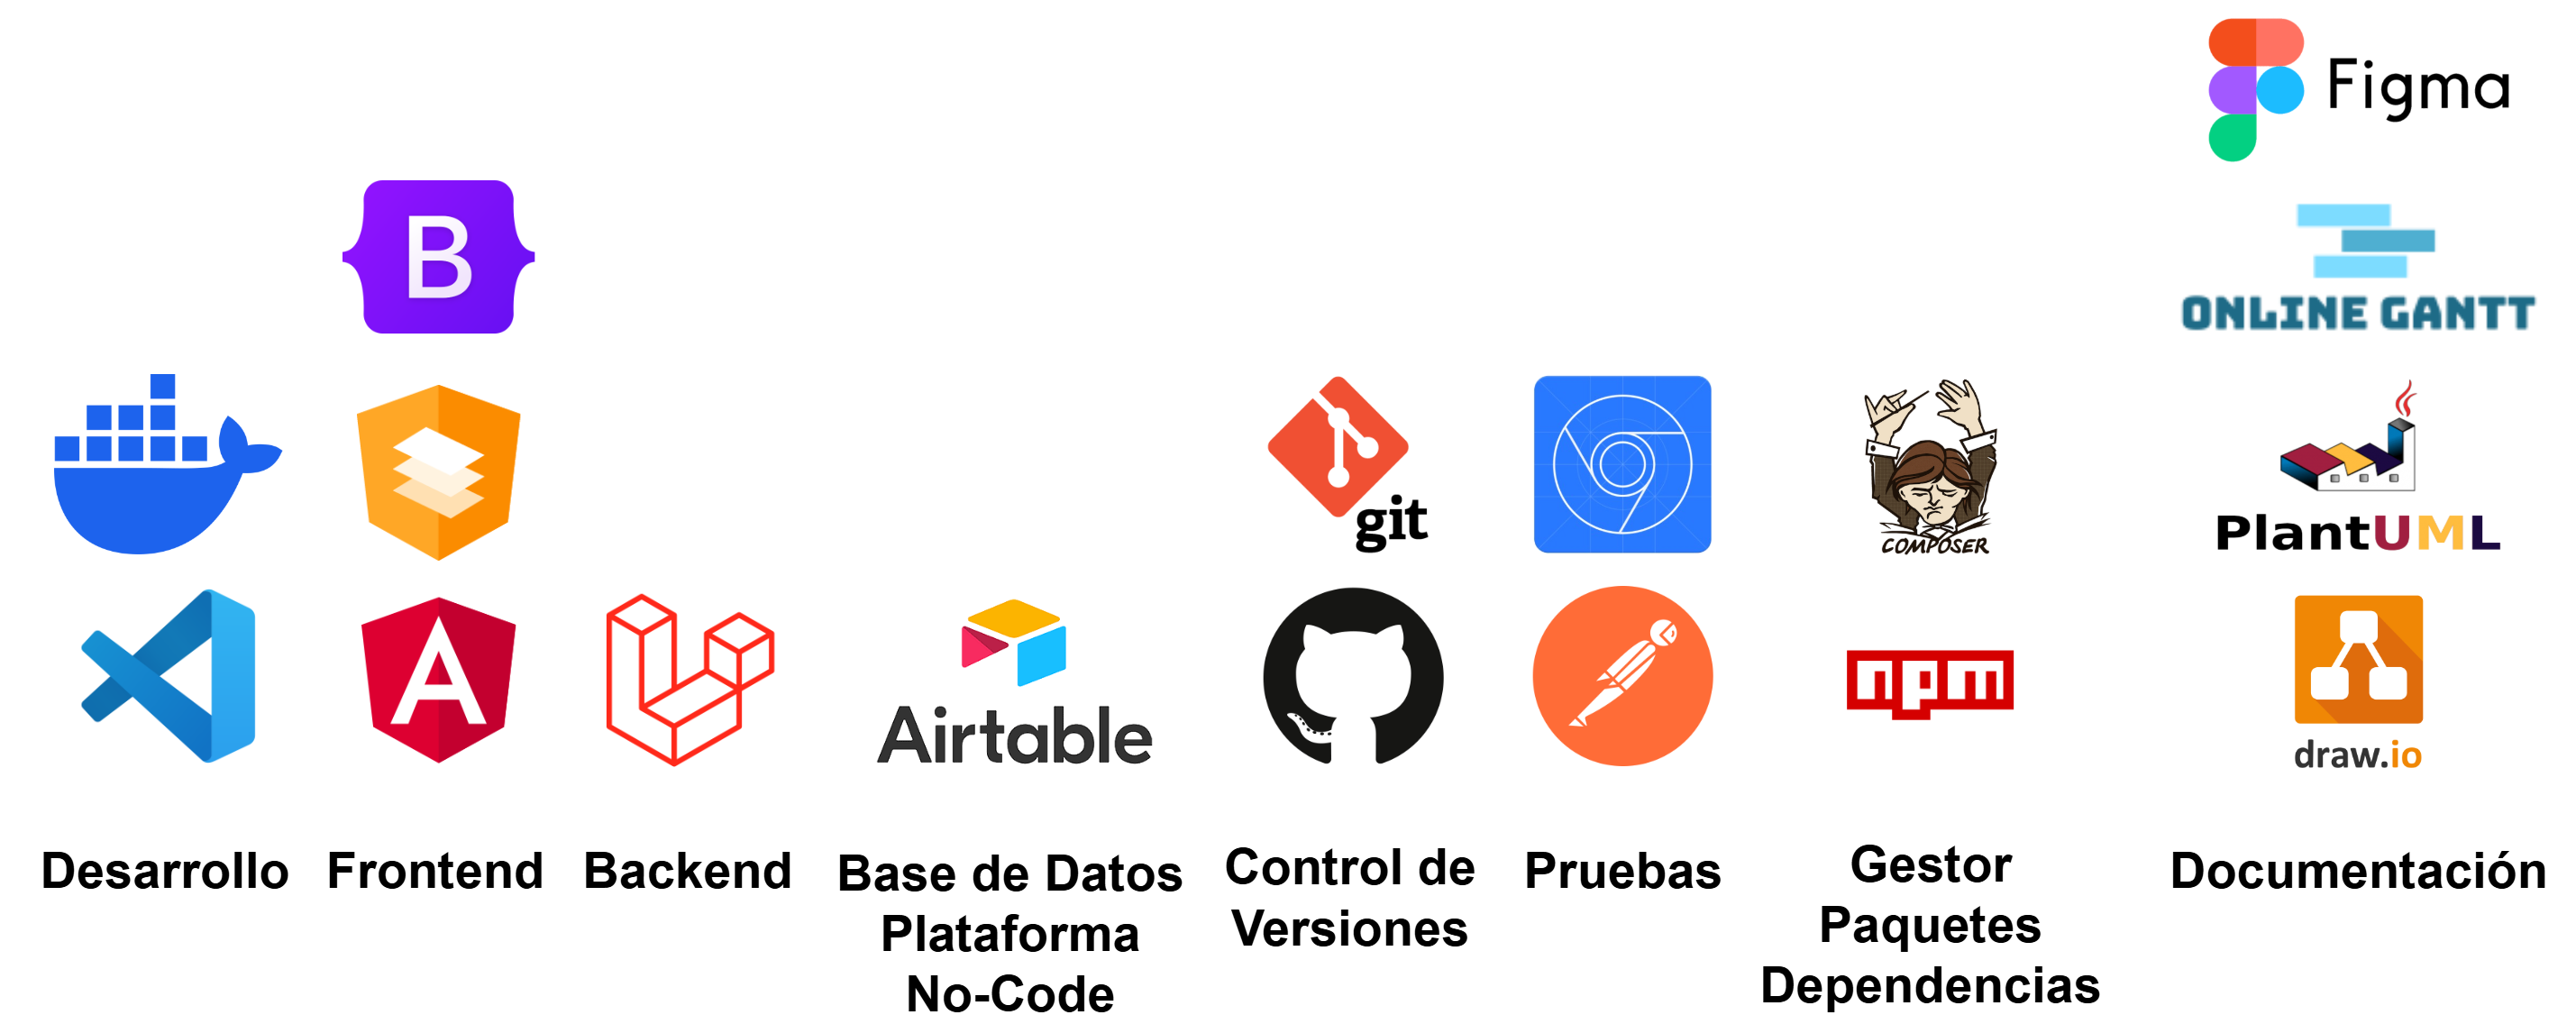
\includegraphics[width = 0.95\textwidth]{Figuras/resumentecnologiasherramientasutilizadas.png}
    \end{center}
    \caption{\label{fig:resumentecnologiasherramientasutilizadas} Resumen de Modelos de Desarrollo y Tecnologías}
\end{figure}

En la Figura ~\ref{fig:resumentecnologiasherramientasutilizadas}, se presenta un resumen visual de todas las tecnologías y herramientas clave seleccionadas para el desarrollo del proyecto \textbf{InmoTable}.


\chapter{InmoTable} 
\label{sec:inmotable}


En este capitulo se describe en profundidad el diseño y la implementación del sistema, abarcando su arquitectura, el modelo de datos y las interfaces de usuario para clientes (web) y agentes (Airtable).


\section{Descripción de la aplicación}


El proyecto \textbf{InmoTable} es una aplicación web de gestión inmobiliaria que implementa una arquitectura híbrida de tres capas para optimizar las operaciones del sector. Consiste en un frontend interactivo desarrollado con Angular para los clientes finales, que les permite buscar propiedades, visualizar detalles y solicitar citas. Este frontend se comunica con un backend robusto construido en Laravel, que actúa como una API segura y el intermediario principal para la gestión de la lógica de negocio y la persistencia de datos.

La singularidad de \textbf{InmoTable} radica en la utilización de Airtable como la base de datos central y la plataforma principal de gestión interna para los agentes inmobiliarios y administradores. Airtable no solo almacena los datos de propiedades, clientes y citas, sino que también provee interfaces visuales \textit{low-code} (formularios, vistas personalizadas, dashboards analíticos) y automatizaciones que permiten a los agentes gestionar eficientemente todas sus operaciones diarias sin necesidad de desarrollo personalizado, ofreciendo una solución rentable y altamente replicable para múltiples inmobiliarias.


\section{Diseño de la arquitectura}


El diseño arquitectónico del sistema \textbf{InmoTable} es una pieza central que define la estructura y el comportamiento de sus componentes. Se ha optado por una arquitectura de tres capas (o N-tier) distribuidas y un enfoque híbrido, buscando un equilibrio óptimo entre la experiencia de usuario para el cliente final, la robustez de la lógica de negocio y la eficiencia en la gestión interna de la inmobiliaria. La Figura ~\ref{fig:estructura-general-aplicacion} ilustra esta estructura general.

\begin{figure}[H]
    \begin{center}
        \includegraphics[width = 0.95\textwidth]{Figuras/estructura-general-aplicacion.png}
    \end{center}
    \caption{\label{fig:estructura-general-aplicacion} Estructura General del Proyecto}
\end{figure}

Esta arquitectura se descompone en las siguientes capas y componentes clave:

\begin{enumerate}

    \item \textbf{Capa de Presentación (Frontend: Aplicación Web para Clientes)}

    Esta capa representa la interfaz directa con los clientes finales (Visitantes Web y Clientes Registrados). Su objetivo es proporcionar una experiencia de usuario moderna, intuitiva y fluida.

    \begin{itemize}
        \item \textbf{Tecnología Principal: Angular} (desarrollado con TypeScript y ejecutado sobre Node.js) \cite{angular2024overview}.
        
        \item \textbf{Librerías de UI/UX:} Se utilizan \textbf{Angular Material} y \textbf{Bootstrap} para estandarizar y acelerar el desarrollo de componentes visuales, garantizando un diseño responsivo y atractivo para diversos dispositivos \cite{angular2024material} \cite{bootstrap2024docs}.
        
        \item \textbf{Funcionalidades:} Permite a los \textbf{Visitantes Web} buscar, filtrar y visualizar listados y detalles de propiedades, así como enviar mensajes de contacto. Los \textbf{Clientes Registrados} pueden además autenticarse y solicitar citas para propiedades.
        
        \item \textbf{Comunicación:} Interactúa con el backend a través de peticiones HTTP a una API RESTful.
    \end{itemize}

\clearpage

    \item \textbf{Capa de Lógica de Negocio/Aplicación (Backend: API RESTful en Laravel)}

    Esta capa es el cerebro del sistema. Actúa como el intermediario seguro y la central de orquestación entre la aplicación web del cliente y la base de datos central de Airtable.

    \begin{itemize}
        \item \textbf{Tecnología Principal: Laravel} (PHP) \cite{laravel2024docs}.
        
        \item \textbf{Entorno de Ejecución:} Se apoya en \textbf{PHP-FPM} para el procesamiento de las solicitudes PHP, servido por \textbf{Nginx}.
        
        \item \textbf{Funcionalidades:}
        
        \begin{itemize}
            \item \textbf{Gestión de Autenticación y Autorización:} Utiliza Laravel \textbf{Passport} para un sistema robusto de autenticación API basado en tokens (OAuth2), gestionando el acceso de clientes, agentes y administradores.

            \item \textbf{Interacción con la Capa de Datos:} Contiene el AirtableService.php, que es el módulo encargado de traducir las solicitudes del frontend en llamadas a la API de Airtable (operaciones CRUD sobre propiedades, citas, clientes, etc.).

            \item \textbf{Validación y Lógica de Negocio:} Aplica reglas de negocio y validaciones de datos antes de interactuar con la capa de persistencia o devolver respuestas al frontend.
        \end{itemize}
        
    \end{itemize}

    \item \textbf{Capa de Datos y Gestión Interna (Airtable: Plataforma para Agentes y Administradores)}

    Esta capa es el corazón de la gestión inmobiliaria para los usuarios internos, diferenciándose por su naturaleza \textit{low-code} y su rica interfaz para la administración del negocio.

    \begin{itemize}
        \item \textbf{Tecnología Principal: Airtable} \cite{airtable2024basics} \cite{airtable2024developers} \cite{airtable2024support}.
        
        \item \textbf{Funcionalidades Clave:}
        
        \begin{itemize}
            \item \textbf{Almacenamiento de Datos:} Contiene todas las tablas estructuradas del negocio inmobiliario: Propiedades, Agentes, Clientes, Citas, Empresas, Usuarios, Contacto.

            \item \textbf{Interfaces de Gestión:} Provee una interfaz visual completa para \textbf{Agentes Inmobiliarios} y \textbf{Administradores}, que incluye:

            \begin{itemize}
                \item \textbf{Vistas Personalizadas:} Para visualizar datos en distintos formatos (calendarios, galerías, mapas).

                \item \textbf{Formularios de Entrada de Datos:} Para el CRUD de entidades (ej. "Nueva Propiedad", "Nueva Cita").

                \item \textbf{Dashboards Analíticos (Airtable Interfaces):} Herramientas de Business Intelligence integradas para el seguimiento del negocio (ej. "Análisis de Stock", "Media de Precios", "Tiempo Medio de Venta", etc.).
            \end{itemize}

            \item \textbf{Automatizaciones:} Gestión de flujos de trabajo automatizados para reducir tareas manuales (ej. envío de notificaciones por email).
        \end{itemize}

        \item \textbf{Comunicación:} Se comunica con el Backend (Laravel) a través de la API de Airtable.
    \end{itemize}

    \item \textbf{Orquestación del Entorno (Docker)}

    \begin{itemize}
        \item \textbf{Tecnología: Docker}  y \textbf{Docker Compose} \cite{docker2024docs}.

        \item \textbf{Rol:} Encapsula las capas de Frontend (servida por Nginx en un contenedor) y Backend (Laravel y PHP-FPM en otro contenedor) en entornos aislados y portables. Esto asegura la consistencia entre el desarrollo y el despliegue, y facilita la replicabilidad de la aplicación.
    \end{itemize}

\end{enumerate}

\textbf{Flujo General de Interacción del Sistema:}

\begin{enumerate}
    \item Los \textbf{Clientes} interactúan directamente con la \textbf{Aplicación Web (Frontend Angular)}.
    
    \item La \textbf{Aplicación Web (Frontend Angular)} realiza peticiones a la \textbf{API RESTful (Backend Laravel)} para obtener y enviar datos.
    
    \item El \textbf{Backend (Laravel API)} procesa estas peticiones, aplica la lógica de negocio y se comunica bidireccionalmente con \textbf{Airtable (Capa de Datos y Gestión Interna)} a través de su API para leer y escribir información.
    
    \item Los \textbf{Agentes Inmobiliarios} y \textbf{Administradores} interactúan directamente con \textbf{Airtable}, utilizando sus interfaces para gestionar propiedades, citas, clientes y acceder a los paneles de análisis y automatizaciones.
\end{enumerate}


\section{Modelo de Datos}


El diseño del modelo de datos es un pilar fundamental en la arquitectura de cualquier sistema de software, ya que define cómo se organiza, se almacena y se relaciona la información crucial del negocio. Para \textbf{InmoTable}, el modelo de datos se ha concebido y materializado en Airtable, aprovechando sus capacidades de base de datos relacional con una interfaz amigable tipo hoja de cálculo. Este enfoque permite una gestión de datos eficiente y flexible por parte de los agentes inmobiliarios, al tiempo que soporta la lógica de la aplicación web.

La Figura ~\ref{fig:diagrama_modelo_de_datos} presenta el diagrama del modelo de datos de \textbf{InmoTable}, donde se visualizan las principales entidades del sistema, sus atributos y las relaciones que las conectan.

\begin{figure}[H]
    \begin{center}
        \includegraphics[width = 0.95\textwidth]{Figuras/diagrama_modelo_de_datos.png}
    \end{center}
    \caption{\label{fig:diagrama_modelo_de_datos} Diagrama del modelo de datos}
\end{figure}

El modelo de datos se compone de las siguientes entidades principales, cada una representando un componente clave de la gestión inmobiliaria:

\begin{enumerate}

    \item \textbf{Entidades del Modelo de Datos}

    \begin{itemize}
        \item \textbf{Agente:} Almacena la información de los agentes inmobiliarios.
    
        \item \textbf{Cita:} Representa las citas o reuniones programadas (ej., visitas a propiedades).
    
        \item \textbf{Cliente:} Contiene la información de los clientes interesados en los servicios de la inmobiliaria.
    
        \item \textbf{Empresa:} Almacena los datos de la inmobiliaria o empresa además de contenido dinámico para la aplicación web (ej., colores principales de la web).
    
        \item \textbf{Propiedad:} El catálogo central de inmuebles gestionados por la inmobiliaria.
    
        \item \textbf{Usuario:} Centraliza las credenciales y roles de acceso al sistema para autenticación.
    
        \item \textbf{Contacto:} Registra los mensajes y consultas recibidas a través del formulario de contacto de la aplicación web.
    \end{itemize}

    \item \textbf{Consideraciones del Modelo de Datos en Airtable}

    La elección de Airtable como plataforma de datos introduce características específicas que refuerzan el modelo:

    \begin{itemize}
        \item \textbf{Interfaz Visual y Flexible:} La naturaleza de spreadsheet de Airtable permite a los agentes visualizar y manipular los datos de manera intuitiva, a la vez que se mantiene la robustez de las relaciones subyacentes. La gestión directa de tablas, formularios e interfaces por usuarios no técnicos es una de sus principales ventajas operacionales.

        \item \textbf{Campos Derivados y Analíticos:} Airtable facilita la creación de campos de fórmula y rollup (ej., Días en el Mercado, recuentos de Citas o Clientes Interesados), que no se almacenan directamente, sino que se calculan a partir de los datos existentes y las relaciones, proporcionando las métricas necesarias para los dashboards analíticos de los agentes.

        \item \textbf{Manejo de Archivos Multimedia:} El campo Fotos en la tabla \texttt{Propiedad} utiliza la capacidad de Airtable para almacenar adjuntos, simplificando la gestión de imágenes de propiedades.
    \end{itemize}

\end{enumerate}


\section{Diseño e implementación}


\subsection{Prototipado de la interfaz}


El prototipado de la interfaz de usuario (UI) es un paso esencial en el proceso de diseño centrado en el usuario, permitiendo visualizar y validar la experiencia del usuario (UX) antes de invertir recursos significativos en el desarrollo. Para \textbf{InmoTable}, esta fase se llevó a cabo utilizando Figma, una herramienta colaborativa de diseño que facilitó la creación de wireframes, mockups de alta fidelidad y prototipos interactivos. El objetivo principal fue obtener una representación visual clara de cómo interactuarían los clientes con la aplicación web, permitiendo recolectar retroalimentación temprana y realizar ajustes en el diseño.

A continuación, se presentan los mockups clave diseñados, seguidos de una justificación de cómo la implementación final pudo diferir.

\subsubsection{Mockup de la Página de Inicio (Landing Page)}

\begin{figure}[H]
    \begin{center}
        \includegraphics[width = 0.95\textwidth]{Figuras/mockup_1_inicio.png}
    \end{center}
    \caption{\label{fig:mockup_1_inicio} Mockup de la Página de Inicio (Landing Page)}
\end{figure}

La figura ~\ref{fig:mockup_1_inicio} representa la primera impresión del usuario al acceder a la aplicación. Típicamente incluiría una sección principal (hero section) con un mensaje de bienvenida o un carrusel de propiedades destacadas, una barra de navegación clara, y posiblemente secciones introductorias a las funcionalidades clave como la búsqueda de propiedades o el contacto.

\subsubsection{Mockup de la Página de Listado de Propiedades}

\begin{figure}[H]
    \begin{center}
        \includegraphics[width = 0.95\textwidth]{Figuras/mockup_2_listado_propiedades.png}
    \end{center}
    \caption{\label{fig:mockup_2_listado_propiedades} Mockup de la Página de Listado de Propiedades}
\end{figure}

La figura ~\ref{fig:mockup_2_listado_propiedades} muestra cómo se visualizarían las propiedades disponibles en un formato de lista o cuadrícula. Incluiría elementos de filtrado y búsqueda en la parte superior o lateral, y tarjetas de propiedad con información esencial como imagen, precio, ubicación y número de habitaciones. Es la interfaz principal para la exploración del inventario.

\subsubsection{Mockup de la Página de Detalle de Propiedad}

\begin{figure}[H]
    \begin{center}
        \includegraphics[width = 0.95\textwidth]{Figuras/mockup_3_detalle_propiedad.png}
    \end{center}
    \caption{\label{fig:mockup_3_detalle_propiedad} Mockup de la Página de Detalle de Propiedad}
\end{figure}

\begin{figure}[H]
    \begin{center}
        \includegraphics[width = 0.95\textwidth]{Figuras/mockup_3_detalle_propiedad_mapa.png}
    \end{center}
    \caption{\label{fig:mockup_3_detalle_propiedad_mapa} Mockup del Mapa de la Página de Detalle de Propiedad}
\end{figure}

Las figuras ~\ref{fig:mockup_3_detalle_propiedad} y ~\ref{fig:mockup_3_detalle_propiedad_mapa} detallan la vista individual de una propiedad. Presentaría una galería de imágenes o un visor principal, una descripción textual completa, características detalladas (superficie, baños, calificación energética), y secciones para solicitar más información o programar una visita.

\subsubsection{Mockup de Formulario de Solicitud de Cita}

\begin{figure}[H]
    \begin{center}
        \includegraphics[width = 0.95\textwidth]{Figuras/mockup_4_pedir_cita.png}
    \end{center}
    \caption{\label{fig:mockup_4_pedir_cita} Mockup de Formulario de Solicitud de Cita}
\end{figure}

La figura ~\ref{fig:mockup_4_pedir_cita} ilustra el formulario diseñado para que los clientes soliciten una cita, presumiblemente para visitar una propiedad. Típicamente incluiría campos para la información de contacto del cliente (nombre, email), la propiedad de interés y los detalles deseados de la cita (fecha, hora, tipo de cita). Es la interfaz principal para formalizar el interés del cliente en un inmueble y ser gestionado por los agentes.


\subsubsection{Mockup de Formulario de Contacto}

\begin{figure}[H]
    \begin{center}
        \includegraphics[width = 0.95\textwidth]{Figuras/mockup_5_contacto.png}
    \end{center}
    \caption{\label{fig:mockup_5_contacto} Mockup de Formulario de Contacto}
\end{figure}

La figura ~\ref{fig:mockup_5_contacto} representa un formulario general para que los usuarios (Visitantes Web o Clientes Registrados) puedan enviar mensajes, consultas o comentarios a la inmobiliaria. Contendría campos para el nombre, email y un área de texto para el mensaje.


\subsubsection{Justificación de las Desviaciones entre Prototipo e Implementación Real}


Es una práctica común y esperable que existan diferencias entre los mockups iniciales y la interfaz final implementada en la aplicación web. Estas desviaciones no representan fallas en el diseño, sino una adaptación necesaria y optimización basada en factores que emergen durante el ciclo de desarrollo ágil y la codificación real. Las principales razones para estas modificaciones en \textbf{InmoTable} incluyen:

\begin{itemize}
    \item \textbf{Restricciones Técnicas y Optimización de la Implementación:} Ciertos elementos de diseño, aunque atractivos en Figma, pueden ser complejos, demandar mucho tiempo o generar problemas de rendimiento al ser implementados en Angular. Las decisiones de implementación final priorizaron la eficiencia, la carga rápida y la estabilidad.

    \item \textbf{Aprovechamiento de Librerías de Componentes (Angular Material y Bootstrap):} Al utilizar frameworks de UI como Angular Material y Bootstrap, la implementación se adhiere a sus componentes prediseñados y estándares de estilo para mantener la consistencia y la velocidad de desarrollo. Esto puede resultar en variaciones visuales respecto a un mockup totalmente personalizado de Figma que no considera las limitaciones o convenciones de estas librerías.

    \item \textbf{Retroalimentación y Pruebas de Usabilidad:} Durante las pruebas internas o simulaciones de interacción con usuarios, se pudieron identificar puntos de fricción o mejoras en la usabilidad que llevaron a ajustes en el layout, la disposición de elementos o los flujos de navegación para hacer la aplicación más intuitiva y fácil de usar para el cliente final.

    \item \textbf{Evolución Natural del Proyecto:} El desarrollo ágil, bajo la metodología Scrum, permite que los requisitos y el diseño evolucionen a medida que se gana comprensión sobre el problema y la solución, llevando a optimizaciones que no eran evidentes en la fase inicial de prototipado.
\end{itemize}

En conclusión, los mockups sirvieron como una guía visual fundamental, pero la implementación real priorizó la viabilidad técnica, la eficiencia del desarrollo y una experiencia de usuario optimizada, adaptándose a las realidades de la codificación y la integración con las herramientas seleccionadas.


\subsection{Diseño de la interfaz}

La fase de diseño de la interfaz ha sido fundamental para materializar la arquitectura y los requisitos de \textbf{InmoTable} en una experiencia de usuario coherente y efectiva. Dada la naturaleza híbrida del sistema, este diseño se ha bifurcado para satisfacer las necesidades específicas de dos perfiles de usuario principales: los clientes finales que interactúan con la aplicación web, y los agentes inmobiliarios y administradores que gestionan las operaciones internas a través de Airtable.

El objetivo ha sido crear una aplicación web intuitiva y visualmente atractiva para el cliente, utilizando Angular Material y Bootstrap para una interfaz moderna y responsiva. Paralelamente, se han configurado potentes interfaces de gestión en Airtable que empoderan a los usuarios internos con herramientas visuales, formularios dinámicos y paneles de análisis sin necesidad de programación.

A continuación, se detalla el diseño de la interfaz de usuario, organizado por los módulos clave del sistema, mostrando cómo cada funcionalidad se aborda en ambas plataformas.


\subsubsection{Módulo: Componentes Globales de la Interfaz del Cliente}


Este módulo describe los elementos de la interfaz de usuario que son omnipresentes o que establecen la primera interacción con la aplicación web para el cliente, proporcionando una base visual y funcional consistente en toda la experiencia de usuario.

\begin{enumerate}
    \item \textbf{Página de Inicio (Home Page)}

    La página de inicio (\texttt{home.component}) es el punto de entrada principal para los \textbf{Visitantes Web} y \textbf{Clientes Registrados}, diseñada para causar una primera impresión impactante y dirigir al usuario hacia las funcionalidades clave del sistema. Esá inspirada en el mockup de la Figura ~\ref{fig:mockup_1_inicio}) y corresponde al requisito funcional que busca ofrecer una experiencia de búsqueda atractiva y funcional.

    \begin{figure}[H]
        \begin{center}
            \includegraphics[width = 0.95\textwidth]{Figuras/inicio.png}
        \end{center}
        \caption{\label{fig:inicio} Página de Inicio}
    \end{figure}

    Tal como se aprecia en la Figura ~\ref{fig:inicio} (imagen inicio.jpg), la página de inicio se caracteriza por:

    \begin{itemize}
         \item \textbf{Sección principal (\texttt{hero section}):} Visualmente atractiva, esta sección contiene un mensaje principal, mencionando directamente el nombre de la inmobiliaria ("InmoTable" en este contexto) y un llamado a la acción claro.

         \item \textbf{Buscador de propiedades integrado:} Directamente en la \texttt{hero section} se ubica un buscador de propiedades con filtros predefinidos (ej., "Tipo de Propiedad", "Zona", "Precio"). Al utilizar este buscador, el usuario será redirigido dinámicamente al Listado de Propiedades, aplicando los filtros seleccionados, lo que agiliza el proceso de búsqueda.

         \item \textbf{Contenido Destacado:} Presenta un resumen de propiedades destacadas o categorías populares, invitando al usuario a explorar el inventario sin necesidad de navegar a una página de listado específica de inmediato.

         \item \textbf{Elementos de Navegación Integrados:} Incluye la barra de navegación en la parte superior y el pie de página en la inferior, manteniendo la coherencia de la interfaz.
    \end{itemize}

    Es importante destacar que la configuración general de colores de la aplicación son configurados dinámicamente. Sus valores se obtienen de campos específicos definidos en la tabla \texttt{Empresa} de Airtable, lo que facilita enormemente la personalización visual y la portabilidad de la aplicación para diferentes inmobiliarias con un mínimo esfuerzo de configuración en el código.

    \begin{figure}[H]
        \begin{center}
            \includegraphics[width = 0.95\textwidth]{Figuras/iniciorojo.png}
        \end{center}
        \caption{\label{fig:iniciorojo} Página de Inicio dinámica}
    \end{figure}

    En la Figura ~\ref{fig:iniciorojo} se visualiza página de inicio de la otra empresa configurada, donde se observa el cambio de título y de colores.

    \item \textbf{Barra de Navegación (Nav / Header)}

    La barra de navegación (\texttt{navbar.component}) es un componente persistente que se mantiene en la parte superior de todas las páginas de la aplicación web, proporcionando acceso constante a las secciones principales del sistema. Visible en la Figura ~\ref{fig:navbar}).

    \begin{figure}[H]
        \begin{center}
            \includegraphics[width = 0.95\textwidth]{Figuras/navbar.png}
        \end{center}
        \caption{\label{fig:navbar} Barra de navegación}
    \end{figure}

    Incluye el logotipo de la inmobiliaria para branding, y un conjunto de enlaces claros que dirigen a los usuarios a las secciones fundamentales: "Propiedades", "Contacto", y opciones de autenticación como "Login" o "Registro". En dispositivos móviles, la navegación se adapta a un menú tipo "hamburguesa" para optimizar el espacio. Como se menciona anteriormente la configuración de colores globales de la aplicación en este componente además el logo y el nombre de la empresa son configurables dinámicamente desde la tabla \texttt{Empresa} de Airtable, lo que garantiza su fácil actualización y coherencia con la imagen de la inmobiliaria.

    Al igual que la Barra de Navegación, la información de contacto y otros datos que se muestran en el pie de página son configurables dinámicamente desde la tabla \texttt{Empresa} de Airtable, lo que garantiza su fácil actualización y coherencia con la imagen de la inmobiliaria.

    \begin{figure}[H]
        \begin{center}
            \includegraphics[width = 0.95\textwidth]{Figuras/navbarrojo.png}
        \end{center}
        \caption{\label{fig:navbarrojo} Barra de navegación dinámica }
    \end{figure}

    En la Figura ~\ref{fig:navbarrojo} se visualiza barra de navegación de la otra empresa configurada, donde se observa el cambio de logo, título y de colores.

    \item \textbf{Pie de Página (Footer)}

    El pie de página (\texttt{footer.component}) es otro componente global que se encuentra en la parte inferior de todas las páginas de la aplicación web. Visible en la Figura ~\ref{fig:footer}.

    \begin{figure}[H]
        \begin{center}
            \includegraphics[width = 0.95\textwidth]{Figuras/footer.png}
        \end{center}
        \caption{\label{fig:footer} Pie de página}
    \end{figure}

\clearpage

    Contiene información esencial de la inmobiliaria (teléfono, dirección, email de contacto), enlaces a políticas legales (privacidad, términos y condiciones) y posibles iconos de redes sociales para la conexión externa. Al igual que la Barra de Navegación, la información de contacto y otros datos que se muestran en el pie de página son configurables dinámicamente desde la tabla \texttt{Empresa} de Airtable, lo que garantiza su fácil actualización y coherencia con la imagen de la inmobiliaria.

    \begin{figure}[H]
        \begin{center}
            \includegraphics[width = 0.95\textwidth]{Figuras/footerrojo.png}
        \end{center}
        \caption{\label{fig:footerrojo} Pie de página dinámica }
    \end{figure}

    En la Figura ~\ref{fig:footerrojo} se visualiza pie de página de la otra empresa configurada, donde se observa el cambio de logo, título, datos de la empresa y de colores.

    \item \textbf{Interfaz para el Agente/Administrador de Gestión de la Base de Datos de Empresa (Grid View) de AirTable}
        
    Este apartado se centra en la gestión de la información global de la inmobiliaria, permitiendo a los administradores centralizar y actualizar los datos corporativos que se utilizan para la configuración dinámica de la aplicación web. Corresponde al requisito funcional que busca facilitar la personalización y portabilidad del sistema.

    \begin{figure}[H]
        \begin{center}
            \includegraphics[width = 0.95\textwidth]{Figuras/tablaempresa1.png}
        \end{center}
        \caption{\label{fig:tablaempresa1} Vista de Cuadrícula (Grid View) de Empresa en AirTable}
    \end{figure}

    \begin{figure}[H]
        \begin{center}
            \includegraphics[width = 0.95\textwidth]{Figuras/tablaempresa2.png}
        \end{center}
        \caption{\label{fig:tablaempresa2} Vista de Cuadrícula (Grid View) de Empresa en AirTable}
    \end{figure}

    Los administradores utilizan la Tabla \texttt{Empresa} en Airtable como su herramienta principal para este fin. La vista de cuadrícula (Grid View), mostrada en las Figuras ~\ref{fig:tablaempresa1} y ~\ref{fig:tablaempresa2}, permite una manipulación directa de campos clave como:

    \begin{itemize}
        \item \textbf{Nombre de la Empresa:} Para el título de la aplicación y el branding general.

        \item \textbf{Logo}: Un campo de adjunto para subir la imagen del logotipo de la inmobiliaria, que se mostrará en la barra de navegación y otras secciones clave.

        \item \textbf{Colores:} Campos (ej., texto con códigos hexadecimales) para definir los colores globales principales de la aplicación (color primario, secundario, etc.), permitiendo personalizar la paleta de colores de la interfaz.

        \item \textbf{Dirección, Teléfono, Email:} Datos de contacto que se replican en el pie de página y otras secciones informativas de la aplicación web.

        \item Otros campos relevantes para la información corporativa o de branding.
    \end{itemize}

    Lo que es fundamental de esta gestión es que todos estos campos son consultados por el backend (Laravel) y luego por el frontend (Angular) para \textbf{configurar dinámicamente} la apariencia y la información de contacto de la aplicación web. Esto significa que cambios en el nombre de la empresa, el logo, los colores o los datos de contacto realizados en Airtable se reflejan automáticamente en la aplicación web \textbf{sin necesidad de modificar código}.

\end{enumerate}


\subsubsection{Módulo: Gestión de Propiedades}


Este módulo es el corazón de la aplicación, permitiendo tanto la visualización de inmuebles por parte de los clientes como su gestión detallada por los agentes.

\begin{enumerate}

    \item \textbf{Interfaz para el Cliente (Aplicación Web)}

    \begin{enumerate}

        \item \textbf{Listado de propiedades}

        La visualización del catálogo de propiedades se implementa a través del componente \texttt{property-list.component}. Inspirada en el mockup de la Figura ~\ref{fig:mockup_2_listado_propiedades}), este listado se presenta en un formato de tarjetas (\texttt{cards}) claras y concisas, organizadas en una cuadrícula (\texttt{grid}) que se adapta dinámicamente al tamaño de la pantalla (diseño responsivo).

        \begin{figure}[H]
            \begin{center}
                \includegraphics[width = 0.90\textwidth]{Figuras/listadopropiedades.png}
            \end{center}
            \caption{\label{fig:listadopropiedades} Listado de propiedades en formato Grid (por defecto)}
        \end{figure}

        Cada tarjeta de propiedad (observada en las Figura ~\ref{fig:listadopropiedades}) contiene la siguiente información esencial para una rápida identificación:

        \begin{itemize}
            \item \textbf{Imagen Principal:} Una fotografía destacada de la propiedad.
            
            \item \textbf{Título:} Nombre de la propiedad.
            
            \item \textbf{Precio:} El precio de venta o alquiler, de manera prominente.
            \item \textbf{Dirección:} Ubicación de la propiedad.
            
            \item \textbf{Características Clave:} Iconos o texto breve que indican atributos importantes como el número de habitaciones, número de baños y m$^2$.
            
            \item \textbf{Tipo de Propiedad:} (ej. Piso, Dúplex).

             \item \textbf{Llamadas a la Acción en Tarjeta:} Cada tarjeta incluye acciones rápidas como "Solicitar Cita" (dirigiendo al \texttt{appointment-form.component}) y "Agregar a Favoritos". El detalle de estas funcionalidades se explicará más adelante en sus respectivas secciones.
        \end{itemize}

        Además de la vista en cuadrícula, la interfaz ofrece una opción para visualizar las propiedades en modo listado (véase Figura ~\ref{fig:listadopropiedadeslist}). Este formato proporciona una disposición más compacta y orientada a texto, ideal para una revisión rápida de múltiples propiedades, mostrando información clave en un estilo similar a una tabla.

        \begin{figure}[H]
            \begin{center}
                \includegraphics[width = 0.95\textwidth]{Figuras/listadopropiedadeslist.png}
            \end{center}
            \caption{\label{fig:listadopropiedadeslist} Listado de propiedades en formato List}
        \end{figure}

        Para facilitar la exploración del extenso inventario, la interfaz incorpora capacidades de filtrado y búsqueda avanzadas (visible en la Figura ~\ref{fig:listadopropiedadesfiltro}).
        
        \begin{figure}[H]
            \begin{center}
                \includegraphics[width = 0.95\textwidth]{Figuras/listadopropiedadesfiltro.png}
            \end{center}
            \caption{\label{fig:listadopropiedadesfiltro} Filtros del listado de propiedades}
        \end{figure}
        
        Los usuarios pueden aplicar filtros dinámicos basados en:
    
        \begin{itemize}
            \item \textbf{Búsqueda general:} Búsqueda por título de la propiedad y/o ubicación geográfica.
            
            \item \textbf{Tipo de Propiedad:} Filtrado por categorías (Piso, Dúplex, Ático, etc.).
            
            \item \textbf{Rango de Precios:} El precio de venta o alquiler, de manera prominente.
            
            \item \textbf{Rango de Precios:} Establecimiento de un presupuesto mínimo y máximo.
            
            \item \textbf{Estado:} Filtrado por estado de disponibilidad (Disponible, Alquilada, Vendida).
        \end{itemize}

        \item \textbf{Detalle de Propiedad}

        La vista de detalle de propiedad, implementada en el \texttt{property-detail} \\ \texttt{.component}, ofrece una inmersión completa en la información de un inmueble seleccionado. Inspirada en el mockup de la Figura ~\ref{fig:mockup_3_detalle_propiedad}) y reflejada en la Figura ~\ref{fig:detallepropiedades}).
        
        \begin{figure}[H]
            \begin{center}
                \includegraphics[width = 0.95\textwidth]{Figuras/detallepropiedades.png}
            \end{center}
            \caption{\label{fig:detallepropiedades} Filtros del listado de propiedades}
        \end{figure}

    \end{enumerate}

    Esta página presenta un diseño limpio y enfocado que prioriza la información visual y detallada:

    \begin{itemize}
        \item \textbf{Galería de Imágenes Principal:} Una sección prominente en la parte superior, que permite al usuario explorar múltiples fotografías de la propiedad en alta resolución, capturando diferentes ángulos y estancias.
        
        \item \textbf{Información Esencial y Precio:} El precio de la propiedad se muestra de manera destacada junto a la dirección y la referencia única.
        
        \item \textbf{Características Detalladas:} Se presenta un resumen visual y textual de las características clave, como el número de habitaciones y baños, superficie en metros cuadrados, y el tipo de propiedad.
        
        \item \textbf{Descripción Completa:} Un bloque de texto extenso proporciona una descripción detallada del inmueble, sus ventajas, distribución y entorno.
        
        \item \textbf{Calificación Energética:} Se incluye una sección dedicada a la calificación energética de la propiedad, con una representación visual del nivel de eficiencia (ej., A, B, C), añadiendo valor informativo al cliente. (Esto se refleja en \texttt{energy-rating} \texttt{.component}).
        
        \item \textbf{Llamadas a la Acción:} La página incorpora llamadas a la acción claras, como botones o enlaces, para que el cliente pueda "Solicitar Cita" para la propiedad (dirigiendo al \texttt{appointment-form.component}) o "Agregar a Favoritos". El detalle de estas funcionalidades se explicará más adelante en sus respectivas secciones.
    \end{itemize}

    La disposición de los elementos busca maximizar la legibilidad y la inmersión del usuario en la información de la propiedad, garantizando que el cliente encuentre todos los detalles que necesita antes de decidir un siguiente paso. El diseño responsivo, logrado con \textbf{Angular Material} y \textbf{Bootstrap}, asegura que esta riqueza de información sea accesible y estéticamente agradable en cualquier dispositivo.

    \item \textbf{Interfaz para el Agente/Administrador (Airtable)}

    Este módulo en Airtable está diseñado para la gestión exhaustiva y colaborativa del inventario de propiedades por parte de los agentes inmobiliarios y administradores. Su objetivo es maximizar la eficiencia en la entrada, manipulación, visualización y análisis de los datos de propiedades sin necesidad de programación. Corresponde principalmente a los requisitos funcionales \textbf{RF 2.1}, \textbf{RF 2.2}, \textbf{RF 2.3}, \textbf{RF 2.4}, \textbf{RF 5.1}, \textbf{RF 5.2}, \textbf{RF 5.3}, \textbf{RF 5.4}, \textbf{RF 5.5}, \textbf{RF 5.6} y \textbf{RF 6.3}.

    \begin{itemize}
        \item \textbf{Gestión de la Base de Datos de Propiedades (Grid View)}

        Los agentes utilizan la interfaz de tabla principal de Airtable como su centro de operaciones para ver, editar, añadir y eliminar registros de propiedades. Esta vista, similar a una hoja de cálculo, permite una manipulación directa y flexible de los datos. Muestra todas las columnas de la tabla \texttt{Propiedades} (referencia, dirección, precio, tipo, superficie, número de habitaciones/baños, descripción, fotos, agente asignado, estado, calificación energética, fecha de publicación) con sus tipos de campo configurados (texto, número, selección única, adjunto, etc.). La Figura ~\ref{fig:gridviewpropiedadesairtable}) ilustra esta configuración, donde se aprecian los campos y la facilidad de edición directa.
    
        \begin{figure}[H]
            \begin{center}
                \includegraphics[width = 0.95\textwidth]{Figuras/gridviewpropiedadesairtable.png}
            \end{center}
            \caption{\label{fig:gridviewpropiedadesairtable} Vista de Cuadrícula (Grid View) de Propiedades en AirTable}
        \end{figure}
        
        \item \textbf{Vista de Listado Compacto:} Una vista de listado optimizada (visible en la Figura ~\ref{fig:listaresumidapropiedadairtable}) que muestra las propiedades en un formato tabular más compacto que la cuadrícula principal, con campos resumidos y esenciales para una revisión rápida de grandes volúmenes de datos. Es ideal para una visualización rápida de la información clave sin necesidad de abrir cada registro.
    
        \begin{figure}[H]
            \begin{center}
                \includegraphics[width = 0.95\textwidth]{Figuras/listaresumidapropiedadairtable.png}
            \end{center}
            \caption{\label{fig:listaresumidapropiedadairtable} Vista de Listado Compacto de Propiedades en AirTable}
        \end{figure}

        Además permite añadir nuevas propiedades directamente desde esta vista mediante un botón o una opción rápida, agilizando el flujo de trabajo de entrada de datos (visible en la Figura ~\ref{fig:listaresumidaaddpropiedadairtable}).

        \begin{figure}[H]
            \begin{center}
                \includegraphics[width = 0.95\textwidth]{Figuras/listaresumidaaddpropiedadairtable.png}
            \end{center}
            \caption{\label{fig:listaresumidaaddpropiedadairtable} Añadir Propiedad en Vista de Listado Compacto de Propiedades en AirTable}
        \end{figure}
    
        \item \textbf{Vista Kanban por Estado de Disponibilidad:} Una vista de tablero tipo Kanban (visible en la Figura ~\ref{fig:kanbanestadodisponibilidadpropiedadairtable}) que organiza las propiedades en columnas según su Estado (ej., "Disponible", "Reservada", "Vendida", "Alquilada"). Esto permite a los agentes arrastrar y soltar propiedades entre estados, visualizando rápidamente el flujo de trabajo de ventas/alquileres y el progreso de cada inmueble.
    
        \begin{figure}[H]
            \begin{center}
                \includegraphics[width = 0.95\textwidth]{Figuras/kanbanestadodisponibilidadpropiedadairtable.png}
            \end{center}
            \caption{\label{fig:kanbanestadodisponibilidadpropiedadairtable} Vista Kanban por Estado de Disponibilidad de Propiedades en AirTable}
        \end{figure}

         \item \textbf{Vista Kanban por Tipo de Propiedad:} Otra vista Kanban (visible en la Figura ~\ref{fig:kanbantipopropiedadairtable}) que clasifica las propiedades por su Tipo de Propiedad (ej., "Apartamentos", "Casas", "Locales"), ofreciendo una visión clara de la composición del inventario por categoría y facilitando la gestión por tipos de inmueble.

         \begin{figure}[H]
            \begin{center}
                \includegraphics[width = 0.95\textwidth]{Figuras/kanbantipopropiedadairtable.png}
            \end{center}
            \caption{\label{fig:kanbantipopropiedadairtable} Vista Kanban por Tipo de Propiedades en AirTable}
        \end{figure}

        \item \textbf{Vista de Galería Visual:} Una vista de galería que presenta las propiedades en un formato tipo tarjeta (\texttt{card}) prominente, con una gran imagen y campos clave debajo (precio, dirección). Es ideal para la navegación visual y para presentaciones rápidas (visible en la Figura ~\ref{fig:galeriapropiedadesairtable}).

         \begin{figure}[H]
            \begin{center}
                \includegraphics[width = 0.95\textwidth]{Figuras/galeriapropiedadesairtable.png}
            \end{center}
            \caption{\label{fig:galeriapropiedadesairtable} Vista de Galería Visual de Propiedades en AirTable}
        \end{figure}
        
    \end{itemize}

\end{enumerate}

\clearpage


\subsubsection{Módulo: Gestión de Clientes y Preferencias}


Este módulo abarca la información de los clientes y sus interacciones con la inmobiliaria, tanto desde la perspectiva del cliente como de la gestión del agente.

\begin{enumerate}

    \item \textbf{Interfaz para el Cliente (Aplicación Web)}

    \begin{enumerate}

        \item \textbf{Autenticación (Inicio de Sesión)}

        Provee un sistema seguro y claro para que los usuarios puedan acceder a funcionalidades personalizadas en la aplicación web. Corresponde al requisito funcional \textbf{RF 1.5}.

        \begin{figure}[H]
            \begin{center}
                \includegraphics[width = 0.95\textwidth]{Figuras/login.png}
            \end{center}
            \caption{\label{fig:login} Inicio de sesión en Aplicación Web}
        \end{figure}

        Representado por la Figura ~\ref{fig:login}, este formulario (\texttt{login.component.html}) está construido directamente en Angular. Requiere credenciales (email/nombre de usuario y contraseña) y, tras una validación exitosa, otorga acceso a las secciones restringidas.

        \item \textbf{Autenticación (Registro)}

        Provee un sistema seguro y claro para que los usuarios puedan crear una cuenta en la aplicación web. Corresponde al requisito funcional \textbf{RF 1.4}.

         \begin{figure}[H]
            \begin{center}
                \includegraphics[width = 0.95\textwidth]{Figuras/registro.png}
            \end{center}
            \caption{\label{fig:registro} Registro en Aplicación Web}
        \end{figure}

        Visible en la Figura ~\ref{fig:registro}, este formulario, a diferencia del login, se ha implementado incrustando un formulario de Airtable. Permite a los nuevos usuarios crear una cuenta de cliente introduciendo datos como nombre, email, teléfono y contraseña. Una vez completado el registro, un registro de usuario se guarda en la tabla \texttt{Usuarios} de Airtable. Adicionalmente, se ha configurado una automatización en Airtable que, tras la creación de este usuario, crea automáticamente un registro de \texttt{Cliente} en la tabla \texttt{Clientes}, asociándolo a dicho usuario. Esto agiliza el flujo de gestión de clientes, delegando el proceso de alta inicial y vinculación al ecosistema de Airtable, cuyo detalle se ampliará en el \texttt{Módulo: Automatizaciones (Visión General)}. Esta elección se justifica por la rapidez y sencillez de implementación que ofrece un formulario \textit{low-code} de Airtable, demostrando una forma eficiente de recopilar datos de nuevos usuarios sin necesidad de un desarrollo a medida completo para esta fase inicial del ciclo de vida del cliente, contrastando con el esfuerzo de los formularios personalizados de Angular.

        \item \textbf{Menú Desplegable (Dropdown) de Usuario Logueado}

        Tras un inicio de sesión exitoso, la interfaz de usuario se actualiza dinámicamente. En la barra de navegación (Nav), se muestra un menú desplegable (visible en la Figura ~\ref{fig:dropdownlogin}) que proporciona al usuario autenticado opciones adicionales, como "Ver mi perfil" o "Cerrar Sesión".

        \begin{figure}[H]
            \begin{center}
                \includegraphics[width = 0.35\textwidth]{Figuras/dropdownlogin.png}
            \end{center}
            \caption{\label{fig:dropdownlogin} Menú Desplegable (Dropdown) de Usuario Logueado en Aplicación Web}
        \end{figure}

        \item \textbf{Mi Perfil}

         Al hacer clic en "Ver mi perfil", el cliente accede a una vista (\texttt{user-form.component} \texttt{.html}) diseñada con componentes Angular nativos (visible en la Figura ~\ref{fig:miperfil}), donde pueden visualizar y editar sus datos personales y preferencias. La construcción de este formulario en Angular contrasta con la simplicidad del registro en Airtable, ilustrando la mayor dificultad y el esfuerzo programático necesario para desarrollar interfaces totalmente personalizadas en Angular, a cambio de un control granular sobre la lógica y la experiencia de usuario.

        \begin{figure}[H]
            \begin{center}
                \includegraphics[width = 0.95\textwidth]{Figuras/miperfil.png}
            \end{center}
            \caption{\label{fig:miperfil} Mi Perfil en Aplicación Web}
        \end{figure}

\clearpage

        \item \textbf{Formulario de Contacto}

         Al hacer clic en "Ver mi perfil", el cliente accede a una vista (\texttt{user-form .component .html}) diseñada con componentes Angular nativos (basado en la Figura ~\ref{fig:mockup_4_pedir_cita} del mockup y visible en la Figura ~\ref{fig:miperfil}), donde pueden visualizar y editar sus datos personales y preferencias. La construcción de este formulario en Angular contrasta con la simplicidad del registro en Airtable, ilustrando la mayor dificultad y el esfuerzo programático necesario para desarrollar interfaces totalmente personalizadas en Angular, a cambio de un control granular sobre la lógica y la experiencia de usuario.

         Proporcionar un canal de comunicación general para cualquier usuario con la inmobiliaria. Corresponde al requisito funcional \textbf{RF 1.6}.

        \begin{figure}[H]
            \begin{center}
                \includegraphics[width = 0.95\textwidth]{Figuras/contacto.png}
            \end{center}
            \caption{\label{fig:contacto} Contacto en Aplicación Web}
        \end{figure}

        Este formulario (visible en la Figura ~\ref{fig:contacto}, correspondiente al \texttt{contact.component}) se ha implementado incrustando un formulario de Airtable. Permite a cualquier usuario, sin necesidad de estar registrado, enviar mensajes o consultas. Contiene campos estándar como nombre, dirección de correo electrónico y un área de texto para el mensaje. Los datos enviados se guardan directamente en la tabla \texttt{Contacto} de Airtable, lo que simplifica la captura de leads y la gestión por parte del equipo interno.

\clearpage

        \item \textbf{Gestión de Propiedades de Interés (Favoritos)}

        Permite a los clientes registrados guardar y acceder fácilmente a las propiedades que les interesan, personalizando su experiencia de búsqueda y seguimiento. Corresponde al requisito funcional \textbf{RF 4.1} y \textbf{RF 4.2} (en cuanto al interés del cliente en propiedades).

        \begin{itemize}
            \item  \textbf{Acción "Agregar a Favoritos":}
            Esta funcionalidad se ofrece directamente en las vistas de listado de propiedades (en las tarjetas) y en la página de detalle de propiedad, mediante un botón o icono intuitivo.
            
            La Figura ~\ref{fig:botonfavoritoquitado} muestra el icono para añadir una propiedad.

            \begin{figure}[H]
                \begin{center}
                    \includegraphics[width = 0.45\textwidth]{Figuras/botonfavoritoquitado.png}
                \end{center}
                \caption{\label{fig:botonfavoritoquitado} Botón Agregar Propiedad Interés (Favoritos) en Aplicación Web}
            \end{figure}
            
            Una vez agregada, el sistema proporciona una confirmación visual (ej., mensaje Figura ~\ref{fig:pripiedadagregadafavorito}).

            \begin{figure}[H]
                \begin{center}
                    \includegraphics[width = 0.45\textwidth]{Figuras/pripiedadagregadafavorito.png}
                \end{center}
                \caption{\label{fig:pripiedadagregadafavorito} Mensaje Agregar Propiedad Interés (Favoritos) en Aplicación Web}
            \end{figure}
            
            Y el icono cambia para reflejar el estado (ej., como en la Figura ~\ref{fig:botonfavoritoagregado}, para "Quitar de Favoritos").

            \begin{figure}[H]
                \begin{center}
                    \includegraphics[width = 0.45\textwidth]{Figuras/botonfavoritoagregado.png}
                \end{center}
                \caption{\label{fig:botonfavoritoagregado} Botón Quitar Propiedad Interés (Favoritos) en Aplicación Web}
            \end{figure}
            
            Si se quita, también hay una confirmación visual (ej., mensaje Figura ~\ref{fig:pripiedadquitadafavorito}). Los clientes autenticados pueden marcar o desmarcar un inmueble como "favorito" con un solo clic.

            \begin{figure}[H]
                \begin{center}
                    \includegraphics[width = 0.45\textwidth]{Figuras/pripiedadquitadafavorito.png}
                \end{center}
                \caption{\label{fig:pripiedadquitadafavorito} Mensaje Quitar Propiedad Interés (Favoritos) en Aplicación Web}
            \end{figure}
            
        \end{itemize}

\clearpage

        \item \textbf{Vista "Mis Propiedades de Interés"}

        Se implementa como una sección dedicada para el cliente (\texttt{property - list - interested .component}) a la que acceden los clientes registrados. Aquí solo se muestran las propiedades que el usuario ha marcado previamente como favoritas. Esta vista ofrece la opción de ver las propiedades en un formato de tarjetas (\texttt{cards}) (Figura ~\ref{fig:mispropiedadesinteres}).
        
        \begin{figure}[H]
            \begin{center}
                \includegraphics[width = 0.95\textwidth]{Figuras/mispropiedadesinteres.png}
            \end{center}
            \caption{\label{fig:mispropiedadesinteres} Mis Propiedad Interés (Favoritos) en formato Grid en Aplicación Web}
        \end{figure}
        
        O en modo listado (Figura ~\ref{fig:mispropiedadesintereslist}), similar a las opciones del listado general de propiedades, pero enfocada en los elementos guardados por el usuario.
        
        \begin{figure}[H]
            \begin{center}
                \includegraphics[width = 0.95\textwidth]{Figuras/mispropiedadesintereslist.png}
            \end{center}
            \caption{\label{fig:mispropiedadesintereslist} Mis Propiedad Interés (Favoritos) en formato List en Aplicación Web}
        \end{figure}
        
        La información de los intereses del cliente se refleja directamente en el campo Interesado en (Propiedades) de la tabla \texttt{Clientes} en Airtable, permitiendo a los agentes tener visibilidad de las preferencias de sus clientes.

    \end{enumerate}

    \item \textbf{Interfaz para el Agente/Administrador (Airtable)}

    Centraliza y gestiona la información de clientes, usuarios y agentes, permitiendo a los usuarios internos mantener una base de datos actualizada y segmentada para la operación del negocio. Corresponde a los requisitos funcionales \textbf{RF 4.1}, \textbf{RF 4.2}, \textbf{RF 6.1} y \textbf{RF 6.3} (en cuanto a la gestión de usuarios y agentes).

    \begin{enumerate}

        \item \textbf{Gestión de la Base de Datos de Clientes (Grid View)}

        Los agentes y administradores utilizan la tabla \texttt{Clientes} en Airtable como su principal herramienta para consultar y editar los datos de los clientes.
        
        \begin{figure}[H]
            \begin{center}
                \includegraphics[width = 0.85\textwidth]{Figuras/gridviewclientesairtable.png}
            \end{center}
            \caption{\label{fig:gridviewclientesairtable} Vista de Cuadrícula (Grid View) de Clientes en AirTable}
        \end{figure}
        
        La vista de cuadrícula (Grid View), mostrada en la Figura ~\ref{fig:gridviewclientesairtable}, permite una manipulación directa de campos como Nombre, Email, Teléfono y Preferencias de vivienda. Se utiliza el Formulario "Nuevo Cliente" para el registro estructurado de nuevos clientes.

        \item \textbf{Vista Kanban de Clientes}

        Una vista Kanban especializada (visible en la Figura ~\ref{fig:kanbanclientesairtable}) organiza los registros de clientes en columnas basadas en el campo Seleccionar (un campo de selección única que clasifica al cliente por su estado en el proceso de ventas: "Nuevo", "Contactado", "Interesado", "Cerrado" o "Perdido").
        
        \begin{figure}[H]
            \begin{center}
                \includegraphics[width = 0.85\textwidth]{Figuras/kanbanclientesairtable.png}
            \end{center}
            \caption{\label{fig:kanbanclientesairtable} Vista Kanban de Clientes en AirTable}
        \end{figure}
        
        Esta vista permite a los agentes arrastrar y soltar clientes entre las diferentes etapas, ofreciendo una representación visual del embudo de ventas y el progreso de la relación con el cliente.
        
        \item \textbf{Gestión de la Base de Datos de Agentes (Grid View)}
        
        Centraliza la información detallada de los agentes inmobiliarios, permitiendo a los administradores gestionar al equipo y sus asignaciones.

        \begin{figure}[H]
            \begin{center}
                \includegraphics[width = 0.95\textwidth]{Figuras/gridviewagentesairtable.png}
            \end{center}
            \caption{\label{fig:gridviewagentesairtable} Vista de Cuadrícula (Grid View) de Agentes en AirTable}
        \end{figure}

        La tabla \texttt{Agentes} en Airtable (visible en la Figura ~\ref{fig:gridviewagentesairtable}) es la herramienta para la gestión de este personal. Muestra campos como Nombre del Agente, Email, Teléfono, DNI, y Empresa a la que pertenecen. También incluye campos vinculados a las Propiedades y Citas que tienen asignadas, ofreciendo una visión consolidada de su carga de trabajo. Se utiliza el Formulario "Nuevo Agente" para registrar nuevos agentes.

        \item \textbf{Gestión de la Base de Datos de Usuarios (Grid View)}
        
        Permite administrar las credenciales de acceso y los roles de todos los usuarios registrados en el sistema (clientes de la web, agentes, administradores), garantizando la seguridad y el control de acceso. Corresponde al requisito funcional \textbf{RF 6.1}.

        \begin{figure}[H]
            \begin{center}
                \includegraphics[width = 0.90\textwidth]{Figuras/gridviewusuariosairtable.png}
            \end{center}
            \caption{\label{fig:gridviewusuariosairtable} Vista de Cuadrícula (Grid View) de Usuarios en AirTable}
        \end{figure}

        La tabla \texttt{Usuarios} en Airtable (visible en la Figura ~\ref{fig:gridviewusuariosairtable}) es la herramienta principal para que los administradores controlen estos registros. Muestra campos como Nombre de Usuario, Email, Contraseña (hash), y Rol. Incluye campos vinculados a \texttt{Agentes} y \texttt{Clientes} para asociar las cuentas de acceso con los perfiles de negocio correspondientes.

        \item \textbf{Gestión de la Base de Datos de Contacto (Grid View)}
        
        Los agentes y administradores utilizan la tabla \texttt{Citas} en Airtable como su principal herramienta para visualizar las consultas de los usuarios anónimos y/o de los clientes registrados.
        
        \begin{figure}[H]
            \begin{center}
                \includegraphics[width = 0.90\textwidth]{Figuras/contactoairtable.png}
            \end{center}
            \caption{\label{fig:contactoairtable} Vista de Cuadrícula (Grid View) de Clientes en AirTable}
        \end{figure}
        
        La vista de cuadrícula (Grid View), mostrada en la Figura ~\ref{fig:contactoairtable}, permite una manipulación directa de campos como Nombre, Email, Teléfono, Mensaje y Estado (Oendiente por defecto). Una vez el Agente haya contactado con el usaurio, pondrá el Estado en Contactado o Rechazado.

    \end{enumerate}

\end{enumerate}


\subsubsection{Módulo: Gestión de Citas}


Este módulo abarca la solicitud de citas por parte de los clientes y la gestión completa de la agenda por los agentes.

\begin{enumerate}

    \item \textbf{Interfaz para el Cliente (Aplicación Web)}

    \begin{enumerate}

        \item \textbf{Formulario de Solicitud de Cita}

        Permite a los clientes (principalmente clientes registrados) solicitar una cita para visitar una propiedad o para otras consultas. Corresponde al requisito funcional \textbf{RF 1.7}.

        \begin{figure}[H]
            \begin{center}
                \includegraphics[width = 0.95\textwidth]{Figuras/formulariopedircita.png}
            \end{center}
            \caption{\label{fig:formulariopedircita} Solicitud de Cita en Aplicación Web}
        \end{figure}

\clearpage

        Este formulario (basado en la Figura ~\ref{fig:mockup_4_pedir_cita} del mockup y visible en Figura ~\ref{fig:formulariopedircita}) se ha implementado incrustando un formulario de Airtable. Se configura para que cargue por defecto la propiedad de interés (pasada por parámetro: \texttt{prefill \_ Propiedad = Record \_ ID} en la URL del formulario de Airtable) y el cliente logueado (pasado por parámetro: \texttt{prefill \_ Cliente = Record \_ ID} en la URL), ocultando estos campos para el usuario final. Esto asegura que la cita esté directamente vinculada a la propiedad y al cliente correcto en la tabla \texttt{Citas} de Airtable, con campos visibles para la fecha, hora, y tipo de cita.
        
        \begin{figure}[H]
            \begin{center}
                \includegraphics[width = 0.95\textwidth]{Figuras/formulariopedircitaairtable.png}
            \end{center}
            \caption{\label{fig:formulariopedircitaairtable} Vista de Cuadrícula (Grid View) de Citas en AirTable}
        \end{figure}
        
        La Figura ~\ref{fig:formulariopedircitaairtable} ilustra la configuración de este formulario en Airtable.

        \item \textbf{Visualización del Calendario de Citas (Cliente)}

        Ofrece a los clientes registrados una vista personalizada de sus citas programadas, permitiéndoles tener un seguimiento visual de sus interacciones con la inmobiliaria.

        \begin{figure}[H]
            \begin{center}
                \includegraphics[width = 0.95\textwidth]{Figuras/calendariocitas.png}
            \end{center}
            \caption{\label{fig:calendariocitas} Calendario de Citas en AirTable}
        \end{figure}

        Esta funcionalidad se implementa incrustando una vista de calendario de Airtable (\texttt{appointment-calendar.component}), la cual es filtrada dinámicamente mediante un parámetro en la URL de Airtable (\texttt{filter \_ Cliente = ID \_ Cliente}). Esto asegura que cada cliente vea únicamente sus propias citas. La Figura ~\ref{fig:calendariocitas} muestra la interfaz del calendario en la aplicación web.

        \begin{figure}[H]
            \begin{center}
                \includegraphics[width = 0.95\textwidth]{Figuras/calendariocitasairtable.png}
            \end{center}
            \caption{\label{fig:calendariocitasairtable} Vista de Calendario de Citas en AirTable}
        \end{figure}

        Y la Figura ~\ref{fig:calendariocitasairtable} ilustra la configuración de este componente en Airtable.

    \end{enumerate}

    \item \textbf{Interfaz para el Agente/Administrador (Airtable)}

    Permitir a los agentes y administradores programar, modificar, dar seguimiento y visualizar todas las citas (de todos los clientes) de manera eficiente, gestionando su agenda y el flujo de interacciones. Corresponde a los requisitos funcionales \textbf{RF 3.1}, \textbf{RF 3.2} y \textbf{RF 3.3}.

    \begin{enumerate}

        \item \textbf{Gestión de la Base de Datos de Citas (Grid View)}

         Los agentes y administradores utilizan esta vista de la tabla \texttt{Citas} en Airtable como la base para una gestión detallada.
        
        \begin{figure}[H]
            \begin{center}
                \includegraphics[width = 0.95\textwidth]{Figuras/gridviewcitasairtable.png}
            \end{center}
            \caption{\label{fig:gridviewcitasairtable} Vista de Cuadrícula (Grid View) de Citas en AirTable}
        \end{figure}
        
        La vista de cuadrícula (Grid View), mostrada en la Figura ~\ref{fig:gridviewcitasairtable}, permite una visualización tabular de todas las citas con campos como "Fecha de la Cita", "Cliente", "Agente", "Propiedad", "Tipo de Cita" y "Estado". Desde aquí, pueden editar directamente cualquier detalle de la cita o acceder al formulario de detalles.

        \item \textbf{Vista de Calendario (para Agentes/Administradores)}

        Los agentes y administradores también utilizan la Vista de Calendario de Airtable (visible en las Figura ~\ref{fig:calendariotablacitasairtable}) para una visión global de todas las citas de la inmobiliaria.

        \begin{figure}[H]
            \begin{center}
                \includegraphics[width = 0.95\textwidth]{Figuras/calendariotablacitasairtable.png}
            \end{center}
            \caption{\label{fig:calendariotablacitasairtable} Vista de Calendario de Citas en AirTable}
        \end{figure}
        
        Esta vista les permite ver la agenda completa, filtrar por agente o por propiedad, y arrastrar/soltar citas para reprogramarlas, optimizando la gestión de tiempo de todo el equipo.

    \end{enumerate}

\end{enumerate}


\subsubsection{Módulo: Análisis de Negocio}


Este módulo es fundamentalmente para agentes y administradores, y se gestiona íntegramente a través de las potentes interfaces de Airtable, proporcionando vistas clave del negocio.

El propósito es transformar los datos brutos en información accionable para la toma de decisiones estratégicas, permitiendo a los usuarios internos monitorear el rendimiento, identificar tendencias y áreas de mejora en el negocio inmobiliario. Corresponde a los requisitos funcionales \textbf{RF 5.1}, \textbf{RF 5.2}, \textbf{RF 5.3}, \textbf{RF 5.4}, \textbf{RF 5.5} y \textbf{RF 5.6}.

A continuación se detallan todas las interfaces creadas en Airtable.

\begin{enumerate}

    \item \textbf{Análisis de Stock}

    En las Figuras ~\ref{fig:interfazairtableanalisisstock} y ~\ref{fig:interfazairtableanalisisstockdetalle} muestra cuadros de mando con métricas agregadas (total de propiedades, disponibles, precio medio, superficie media) y gráficos de distribución de propiedades por tipo y estado, ofreciendo una visión ejecutiva del inventario.

    \begin{figure}[H]
        \begin{center}
            \includegraphics[width = 0.95\textwidth]{Figuras/interfazairtableanalisisstock.png}
        \end{center}
        \caption{\label{fig:interfazairtableanalisisstock} Interfaz de Análisis de Stock en AirTable}
    \end{figure}

    \begin{figure}[H]
        \begin{center}
            \includegraphics[width = 0.95\textwidth]{Figuras/interfazairtableanalisisstockdetalle.png}
        \end{center}
        \caption{\label{fig:interfazairtableanalisisstockdetalle} Detalle de Interfaz de Análisis de Stock en AirTable}
    \end{figure}

    \item \textbf{Media de Precios por Tipo de Inmueble}

    En las Figuras ~\ref{fig:interfazairtablemediapreciostipo}, ~\ref{fig:interfazairtablemediapreciostipodetalle} y ~\ref{fig:interfazairtablemediapreciostipofiltro} muestra gráficos de barras que comparan los precios promedio entre diferentes tipos de propiedades (ej. apartamentos vs. casas), facilitando el análisis de tendencias de mercado y la valoración.

    \begin{figure}[H]
        \begin{center}
            \includegraphics[width = 0.95\textwidth]{Figuras/interfazairtablemediapreciostipo.png}
        \end{center}
        \caption{\label{fig:interfazairtablemediapreciostipo} Interfaz de Media de Precios por Tipo de Inmueble en AirTable}
    \end{figure}

    \begin{figure}[H]
        \begin{center}
            \includegraphics[width = 0.95\textwidth]{Figuras/interfazairtablemediapreciostipodetalle.png}
        \end{center}
        \caption{\label{fig:interfazairtablemediapreciostipodetalle} Detalle de Interfaz de Media de Precios por Tipo de Inmueble en AirTable}
    \end{figure}

    \begin{figure}[H]
        \begin{center}
            \includegraphics[width = 0.95\textwidth]{Figuras/interfazairtablemediapreciostipofiltro.png}
        \end{center}
        \caption{\label{fig:interfazairtablemediapreciostipofiltro} Filtro de Interfaz de Media de Precios por Tipo de Inmueble en AirTable}
    \end{figure}

    \item \textbf{Visitas por Propiedad}

    En las Figuras ~\ref{fig:interfazairtablevisitaspropiedad} y ~\ref{fig:interfazairtablevisitaspropiedaddetalle} muestra listados y contadores que muestran el interés generado por cada inmueble (número de citas asociadas), permitiendo identificar las propiedades más demandadas.

    \begin{figure}[H]
        \begin{center}
            \includegraphics[width = 0.95\textwidth]{Figuras/interfazairtablevisitaspropiedad.png}
        \end{center}
        \caption{\label{fig:interfazairtablevisitaspropiedad} Interfaz de Visitas por Propiedad en AirTable}
    \end{figure}

    \begin{figure}[H]
        \begin{center}
            \includegraphics[width = 0.95\textwidth]{Figuras/interfazairtablevisitaspropiedaddetalle.png}
        \end{center}
        \caption{\label{fig:interfazairtablevisitaspropiedaddetalle} Detalle de Interfaz de Visitas por Propiedad en AirTable}
    \end{figure}

    \item \textbf{Visitas Programadas}

    En las Figuras ~\ref{fig:interfazairtablevisitasprogramadas}, ~\ref{fig:interfazairtablevisitasprogramadasdetallesemana} y ~\ref{fig:interfazairtablevisitasprogramadasdetallemes} muestra resúmenes y gráficos de citas por estado y día, complementando la vista de calendario para una comprensión rápida de la carga de trabajo y el progreso de las citas.

    \begin{figure}[H]
        \begin{center}
            \includegraphics[width = 0.95\textwidth]{Figuras/interfazairtablevisitasprogramadas.png}
        \end{center}
        \caption{\label{fig:interfazairtablevisitasprogramadas} Interfaz de Visitas Programadas en AirTable}
    \end{figure}

    \begin{figure}[H]
        \begin{center}
            \includegraphics[width = 0.95\textwidth]{Figuras/interfazairtablevisitasprogramadasdetallesemana.png}
        \end{center}
        \caption{\label{fig:interfazairtablevisitasprogramadasdetallesemana} Detalle por semana de Interfaz de Visitas Programadas en AirTable}
    \end{figure}

    \begin{figure}[H]
        \begin{center}
            \includegraphics[width = 0.95\textwidth]{Figuras/interfazairtablevisitasprogramadasdetallemes.png}
        \end{center}
        \caption{\label{fig:interfazairtablevisitasprogramadasdetallemes} Detalle por mes de Interfaz de Visitas Programadas en AirTable}
    \end{figure}

    \item \textbf{Tiempo Medio de Venta}

    En las Figuras ~\ref{fig:interfazairtabletiempomedioventa}, ~\ref{fig:interfazairtabletiempomedioventadetalle} y ~\ref{fig:interfazairtabletiempomedioventadetalledias} muestra métricas y gráficos sobre la eficiencia en la venta o alquiler de propiedades (días en el mercado por tipo de propiedad), lo que ayuda a identificar cuellos de botella.

    \begin{figure}[H]
        \begin{center}
            \includegraphics[width = 0.95\textwidth]{Figuras/interfazairtabletiempomedioventa.png}
        \end{center}
        \caption{\label{fig:interfazairtabletiempomedioventa} Interfaz de Tiempo Medio de Venta en AirTable}
    \end{figure}

    \begin{figure}[H]
        \begin{center}
            \includegraphics[width = 0.95\textwidth]{Figuras/interfazairtabletiempomedioventadetalle.png}
        \end{center}
        \caption{\label{fig:interfazairtabletiempomedioventadetalle} Detalle de Interfaz de Tiempo Medio de Venta en AirTable}
    \end{figure}

    \begin{figure}[H]
        \begin{center}
            \includegraphics[width = 0.95\textwidth]{Figuras/interfazairtabletiempomedioventadetalledias.png}
        \end{center}
        \caption{\label{fig:interfazairtabletiempomedioventadetalledias} Detalle de Interfaz de Tiempo Medio de Venta en AirTable}
    \end{figure}

    \item \textbf{Propiedades con Baja Rotación}

    En las Figuras ~\ref{fig:interfazairtablepropiedadesbajarotacion} y ~\ref{fig:interfazairtablepropiedadesbajarotaciondisponible} muestra un listado específico de inmuebles que requieren atención especial por su prolongado tiempo en el mercado, con métricas clave para la gestión proactiva.

    \begin{figure}[H]
        \begin{center}
            \includegraphics[width = 0.95\textwidth]{Figuras/interfazairtablepropiedadesbajarotacion.png}
        \end{center}
        \caption{\label{fig:interfazairtablepropiedadesbajarotacion} Interfaz de Propiedades con Baja Rotación en AirTable}
    \end{figure}

    \begin{figure}[H]
        \begin{center}
            \includegraphics[width = 0.95\textwidth]{Figuras/interfazairtablepropiedadesbajarotaciondisponible.png}
        \end{center}
        \caption{\label{fig:interfazairtablepropiedadesbajarotaciondisponible} Propiedades Disponibles con Baja Rotación en AirTable}
    \end{figure}

    \item \textbf{Propiedades}

    En las Figuras ~\ref{fig:interfazairtablepropiedades} y ~\ref{fig:interfazairtablepropiedadesdisponible} muestra gráficos visuales que representan la proporción de propiedades en diferentes estados (ej., "Disponible", "Alquilada", "Vendida"). Esto proporciona una visión rápida de la liquidez y el estado general del inventario, complementando los gráficos por tipo de propiedad.

    \begin{figure}[H]
        \begin{center}
            \includegraphics[width = 0.95\textwidth]{Figuras/interfazairtablepropiedades.png}
        \end{center}
        \caption{\label{fig:interfazairtablepropiedades} Interfaz de Propiedades en AirTable}
    \end{figure}

    \begin{figure}[H]
        \begin{center}
            \includegraphics[width = 0.95\textwidth]{Figuras/interfazairtablepropiedadesdisponible.png}
        \end{center}
        \caption{\label{fig:interfazairtablepropiedadesdisponible} Detalle de Interfaz de Propiedades Disponibles en AirTable}
    \end{figure}

    \item \textbf{Tipo de Propiedades}

    En las Figuras ~\ref{fig:interfazairtabletipopropiedades} y ~\ref{fig:interfazairtabletipopropiedadespiso} muestra gráficos que muestran la composición del inventario por categorías (ej. Apartamentos, Casas), lo que ayuda a la estrategia de adquisición y venta.

    \begin{figure}[H]
        \begin{center}
            \includegraphics[width = 0.95\textwidth]{Figuras/interfazairtabletipopropiedades.png}
        \end{center}
        \caption{\label{fig:interfazairtabletipopropiedades} Interfaz de Tipo de Propiedades en AirTable}
    \end{figure}

    \begin{figure}[H]
        \begin{center}
            \includegraphics[width = 0.95\textwidth]{Figuras/interfazairtabletipopropiedadespiso.png}
        \end{center}
        \caption{\label{fig:interfazairtabletipopropiedadespiso} Detalle de Interfaz de Tipo de Propiedades en AirTable}
    \end{figure}

\end{enumerate}


\subsubsection{Módulo: Automatizaciones (Visión General)}


Este módulo describe la capa de automatización de flujos de trabajo que complementa las interfaces, operando en segundo plano para aumentar la eficiencia del sistema y mejorar la comunicación. Corresponde a los requisitos funcionales\textbf{ RF 3.3}, \textbf{RF 6.2}.

Las automatizaciones configuradas directamente en Airtable son fundamentales para optimizar las operaciones diarias de los agentes inmobiliarios, reducir tareas repetitivas y garantizar una comunicación y un seguimiento eficientes. Aprovechan las capacidades low-code de Airtable para delegar lógica compleja, reduciendo la necesidad de desarrollo de código personalizado en el backend y frontend.

La interfaz de automatizaciones de Airtable permite definir flujos de trabajo mediante disparadores (triggers), condiciones y acciones, de forma visual. Se han implementado varias automatizaciones clave:

\begin{enumerate}

    \item \textbf{Notificar a Agente cuando Propiedad "Vendida":} El propósito es asegurar que el agente responsable de una propiedad reciba una notificación inmediata cuando el estado de la misma cambia a "Vendida", permitiendo una respuesta y un cierre de gestión ágiles.

    \begin{figure}[H]
        \begin{center}
            \includegraphics[width = 0.95\textwidth]{Figuras/automatizacionnotificaragentepropiedadvendida.png}
        \end{center}
        \caption{\label{fig:automatizacionnotificaragentepropiedadvendida} Automatización Notificar Agente Propiedad Vendida en AirTable}
    \end{figure}

    La automatización se activa "Cuando un registro en la tabla \texttt{Propiedades} coincide con ciertas condiciones" (disparador). La condición específica es que el campo \texttt{Estado} de una propiedad sea establecido a "Vendida". La acción es "Enviar un correo electrónico" al email del \texttt{Agente Asignado} de la propiedad. La Figura ~\ref{fig:automatizacionnotificaragentepropiedadvendida} muestra la configuración visual de esta automatización en Airtable.

    \begin{figure}[H]
        \begin{center}
            \includegraphics[width = 0.95\textwidth]{Figuras/emailautomatizacionnotificaragentepropiedadvendida.png}
        \end{center}
        \caption{\label{fig:emailautomatizacionnotificaragentepropiedadvendida} Email de Automatización Notificar Agente Propiedad Vendida en AirTable}
    \end{figure}

    Y la Figura ~\ref{fig:emailautomatizacionnotificaragentepropiedadvendida} muestra el correo electrónico enviado al Agente notificando que la Propiedad ha sido vendida.
    
    \item \textbf{Notificar a Agente cambio precio Propiedad:} El propósito es informar proactivamente al agente asignado sobre cualquier modificación en el precio de una propiedad bajo su gestión, garantizando que siempre manejen la información más actualizada.

    \begin{figure}[H]
        \begin{center}
            \includegraphics[width = 0.95\textwidth]{Figuras/automatizacionnotificaragentecambiopreciopropiedad.png}
        \end{center}
        \caption{\label{fig:automatizacionnotificaragentecambiopreciopropiedad} Automatización Notificar Agente Cambio Precio Propiedad en AirTable}
    \end{figure}

    El disparador es "Cuando un registro en la tabla \texttt{Propiedades} es actualizado", con la condición de que el campo \texttt{Precio} "ha cambiado". La acción subsiguiente es "Enviar un correo electrónico" al \texttt{Agente Asignado}. La Figura ~\ref{fig:automatizacionnotificaragentecambiopreciopropiedad} ilustra esta configuración.

    \begin{figure}[H]
        \begin{center}
            \includegraphics[width = 0.95\textwidth]{Figuras/emailautomatizacionnotificaragentecambiopreciopropiedad.png}
        \end{center}
        \caption{\label{fig:emailautomatizacionnotificaragentecambiopreciopropiedad} Email de Automatización Notificar Agente Cambio Precio Propiedad en AirTable}
    \end{figure}

    Y la Figura ~\ref{fig:emailautomatizacionnotificaragentecambiopreciopropiedad} muestra el correo electrónico enviado al Agente notificando el cambio de precio de una Propiedad.

    \item \textbf{Al crear nuevo Cliente, asignar Agente:} El propósito es simplificar la asignación inicial de responsabilidades a los nuevos clientes captados, garantizando que cada nuevo lead tenga un agente de referencia.

    \begin{figure}[H]
        \begin{center}
            \includegraphics[width = 0.95\textwidth]{Figuras/automatizacionasignaragentealcrearnuevocliente.png}
        \end{center}
        \caption{\label{fig:automatizacionasignaragentealcrearnuevocliente} Automatización Asignar Agente al Crear Nuevo Cliente en AirTable}
    \end{figure}

    La automatización se dispara "Cuando se crea un registro en la tabla \texttt{Clientes}. La acción es "Actualizar registro" en la misma tabla \texttt{Clientes}, asignando automáticamente un \texttt{Agente} predefinido o siguiendo una lógica de asignación (ej., ronda, menos asignaciones). La Figura ~\ref{fig:automatizacionasignaragentealcrearnuevocliente} muestra la configuración.

    \item \textbf{Al crear nuevo Usuario, crea y asigna un nuevo Cliente:} El propósito es sincronizar automáticamente el registro de usuarios de la aplicación web con la base de datos de clientes de la inmobiliaria, facilitando la gestión integral del perfil del cliente.

    \begin{figure}[H]
        \begin{center}
            \includegraphics[width = 0.95\textwidth]{Figuras/automatizacionasignanuevoclientealcrearnuevousuario.png}
        \end{center}
        \caption{\label{fig:automatizacionasignanuevoclientealcrearnuevousuario} Automatización Asigna nuevo Cliente al Crear nuevo Usuario en AirTable}
    \end{figure}

    Esta automatización se activa "Cuando se crea un registro en la tabla \texttt{Usuarios} (el registro proviene del formulario de registro incrustado en la web, Figura ~\ref{fig:registro}). Las acciones subsecuentes incluyen "Actualizar registro" (posiblemente para establecer un \texttt{Rol} o \texttt{Estado} por defecto en la tabla \texttt{Usuarios}), "Crear registro" en la tabla \texttt{Clientes} con los datos del nuevo usuario, y "Enviar un correo electrónico" al usuario registrado (para la bienvenida o activación de cuenta, tal como se discutió previamente, preferiblemente con un enlace seguro para establecer contraseña). La Figura ~\ref{fig:automatizacionasignanuevoclientealcrearnuevousuario} ilustra este flujo.

    \begin{figure}[H]
        \begin{center}
            \includegraphics[width = 0.95\textwidth]{Figuras/emailautomatizacionasignanuevoclientealcrearnuevousuario.png}
        \end{center}
        \caption{\label{fig:emailautomatizacionasignanuevoclientealcrearnuevousuario} Email de Automatización Asigna nuevo Cliente al Crear nuevo Usuario en AirTable}
    \end{figure}

    Y la Figura ~\ref{fig:emailautomatizacionasignanuevoclientealcrearnuevousuario} muestra el correo electrónico enviado al usuario que se ha registrado.

\end{enumerate}


\subsubsection{Módulo: Gestión de Cuentas de Usuario y Roles de Acceso (Airtable)}

Este módulo es administrado principalmente por el Administrador a través de Airtable, controlando los accesos del personal. Se centra específicamente en la gestión de las credenciales de acceso y los niveles de permiso de los colaboradores que utilizan la base de datos de Airtable para la gestión interna de la inmobiliaria.

\begin{figure}[H]
    \begin{center}
        \includegraphics[width = 0.95\textwidth]{Figuras/gestionusuariosinternosrolesairtable.png}
    \end{center}
    \caption{\label{fig:gestionusuariosinternosrolesairtable} Gestión de Cuentas de Usuario y Roles de Acceso en Airtable}
\end{figure}

Los administradores utilizan la interfaz de gestión de colaboradores de Airtable (visible en la Figura ~\ref{fig:gestionusuariosinternosrolesairtable}) como su herramienta principal para controlar estos registros. Esta interfaz muestra a los usuarios internos por su email, nombre, última actividad y, crucialmente, su \texttt{Rol} asignado dentro de Airtable.

\textbf{Roles en Airtable:} La gestión de usuarios se basa en los roles nativos de Airtable, que definen sus capacidades:

\begin{itemize}
    \item \textbf{Administrador (ACT-04):} En Airtable, estos usuarios se corresponden con roles de alto nivel como \textbf{Propietario (Owner)} o \textbf{Creador (Creator)}. Tienen control total sobre la base de datos, incluyendo la capacidad de añadir/eliminar colaboradores, modificar la estructura de las tablas, gestionar interfaces y automatizaciones, y acceder a todos los datos.

    \item \textbf{Agente (ACT-03):} Se corresponden con el rol de \textbf{Editor} en Airtable. Pueden ver y modificar datos en las tablas a las que se les ha dado acceso, añadir registros, usar formularios e interfaces, pero no tienen control sobre la estructura de la base o la administración de usuarios y configuración avanzada.
\end{itemize}





\subsection{Flujo de la aplicación}


En este apartado se va a analizar el funcionamiento interno de algunas de las funcionalidades de nuestro sistema, centrándose en el flujo de cargar el formulario de cita, ya que este es fundamental para mostrar la comunicación de la interfaz de la aplicación web con la API de Airtable, el flujo de actualizar usuario para comprender cómo se relaciona el frontend con el backend. Y, además, se analizará la funcionalidad de añadir una propiedad a favoritos.


\subsubsection{Flujo de cargar el Formulario de Cita}


Este flujo es un ejemplo destacado de cómo la aplicación InmoTable aprovecha la flexibilidad de Airtable para funcionalidades orientadas al cliente, minimizando el desarrollo de código personalizado. Se centra en el proceso que un cliente sigue para solicitar una cita para una propiedad.

\begin{itemize}
    \item \textbf{Carga del Formulario:} Cuando un \textbf{Cliente Registrado} (ACT-02) navega a la página de detalle de una propiedad y decide solicitar una cita, la aplicación web (\texttt{Frontend Angular}) no renderiza un formulario Angular personalizado. En su lugar, construye dinámicamente una URL para un formulario incrustado de Airtable. Esta URL se configura para precargar automáticamente los campos \texttt{Propiedad} (utilizando el \texttt{Record \_ ID} de la propiedad actual) y \texttt{Cliente} (utilizando el \texttt{Record \_ ID} del cliente logueado) mediante parámetros prefill\_ en la URL (ej. \texttt{https://airtable.com/ ... / form ? prefill \_ Propiedad = reciFQKpKH26ZbDd5 \& prefill \_ Cliente =} \\ \texttt{recrq9z2GFijDLWIe}). 
    Estos campos se ocultan en el formulario para el usuario final, garantizando que los datos críticos se asocien correctamente sin intervención manual.

    \item \textbf{Visualización e Interacción:} La aplicación web incrusta este formulario de Airtable (visible en la Figura ~\ref{fig:diagramasecuenciasformulariopedircitaairtable}). El cliente interactúa con los campos visibles del formulario, como la fecha, hora y el tipo de cita, así como cualquier comentario adicional.

    \item \textbf{Envío del Formulario:} Al hacer clic en el botón 'Guardar' (o 'Enviar'), el formulario de Airtable envía los datos directamente a la base de datos de Airtable. La interfaz de Airtable gestiona la persistencia de los datos, registrando la nueva cita en la tabla \texttt{Citas}.

    \item \textbf{Confirmación:} Airtable devuelve una respuesta de éxito al formulario incrustado, y el cliente recibe una confirmación visual en la interfaz web.
\end{itemize}

\textbf{Justificación de la Implementación:}

La decisión de utilizar un formulario incrustado de Airtable para la solicitud de citas por parte del cliente (RF 1.7) se basa en la rapidez y simplicidad de implementación. Permite una integración directa con la base de datos de Airtable para la captura de datos, evitando la necesidad de programar un formulario complejo en Angular, la lógica de validación y la comunicación con la API de Laravel y, a su vez, con la API de Airtable para la inserción del registro. Esto contrasta con el esfuerzo requerido para los formularios nativos de Angular como "Mi Perfil". Este enfoque demuestra la eficiencia en el desarrollo y el ahorro de tiempo al delegar funcionalidades de recolección de datos a una plataforma \textit{low-code}.

\begin{figure}[H]
    \begin{center}
        \includegraphics[width = 0.95\textwidth]{Figuras/diagramasecuenciasformulariopedircitaairtable.png}
    \end{center}
    \caption{\label{fig:diagramasecuenciasformulariopedircitaairtable} Diagrama Secuencias - Formulario Pedir Cita AirTable}
\end{figure}


\subsubsection{Flujo de Actualización de Datos de Usuario (Cliente)}


Este flujo ilustra la comunicación bidireccional entre el frontend, el backend y la capa de datos de Airtable para la gestión de la información personal de un cliente autenticado.

\begin{itemize}
    \item \textbf{Inicio de la Edición:} Un \textbf{Cliente Registrado} (ACT-02), después de iniciar sesión, accede a la sección "Mi Perfil" en la aplicación web. Esta interfaz (\texttt{user-form.component .html}) (visible en la Figura ~\ref{fig:diagramasecuenciasformularioeditarperfilusuario}), construida con componentes Angular nativos, le permite visualizar y modificar sus datos personales (nombre, teléfono, email y contraseña).

    \item \textbf{Envío de Datos al Backend:} Al hacer clic en 'Guardar Cambios', la aplicación web (\texttt{Frontend Angular}) envía una petición HTTP (\texttt{PATCH} o \texttt{PUT}) al endpoint \texttt{/api/user/{id}} del \texttt{Backend (Laravel API)}, incluyendo el ID del usuario y los datos modificados.

    \item \textbf{Validación y Lógica del Backend:} El \texttt{Backend (Laravel API)} recibe la petición. Primero, realiza una validación exhaustiva de los datos recibidos. Si la validación es exitosa, el backend consulta la tabla \texttt{Usuarios} de Airtable (a través del \texttt{AirtableService.php}) para verificar la existencia del usuario y obtener su \texttt{Record ID} en Airtable

    \item \textbf{Actualización en Airtable:} Con el \texttt{Record ID} de Airtable, el \texttt{Backend (Laravel API)} procede a enviar una petición \texttt{PATCH} a la API de Airtable para actualizar la información del usuario en su registro correspondiente en la tabla \texttt{Usuarios}. Esto incluye la actualización del \texttt{password \_ hash} si la contraseña fue modificada.

    \item \textbf{Respuesta del Sistema:} Si la operación de actualización en Airtable se completa correctamente, Airtable responde con éxito al \texttt{Backend (Laravel API)}. El backend, a su vez, devuelve una respuesta al \texttt{Frontend Angular} indicando \texttt{success: true}. En caso de que el usuario no exista o la validación de datos falle, el backend enviará una respuesta \texttt{success: false} o un mensaje de error detallado.
\end{itemize}

\textbf{Justificación de la Implementación:}

Este flujo demuestra el rol crítico del backend de Laravel en la seguridad (validación, autenticación con Passport) y la orquestación de las operaciones CRUD con Airtable para datos sensibles como los de usuario. A diferencia del formulario de registro incrustado, la gestión del perfil requiere un control más granular sobre la lógica de negocio y la validación en el servidor, lo que justifica la implementación de un formulario nativo en Angular y la lógica de backend en Laravel para esta funcionalidad.

\begin{figure}[H]
    \begin{center}
        \includegraphics[width = 0.95\textwidth]{Figuras/diagramasecuenciasformularioeditarperfilusuario.png}
    \end{center}
    \caption{\label{fig:diagramasecuenciasformularioeditarperfilusuario} Diagrama Secuencias - Formulario Editar Perfil Usuario}
\end{figure}


\subsubsection{Flujo de Gestión de Propiedades Favoritas (Cliente)}


Este flujo detalla cómo un \textbf{Cliente Registrado} (ACT-02) puede gestionar su lista de propiedades favoritas desde la aplicación web, una funcionalidad que se refleja directamente en la base de datos de Airtable para la visibilidad del agente.

\begin{itemize}
    \item \textbf{Acción del Usuario:} Cuando un cliente autenticado selecciona la opción "Agregar a Favoritos" (o "Quitar de Favoritos") en el listado o detalle de una propiedad (visible en la Figura ~\ref{fig:diagramasecuenciasbotoninterespropiedad}), la aplicación web (\texttt{Frontend Angular}) envía una petición HTTP (\texttt{POST} o \textit{PATCH}) al endpoint \texttt{api/favorites} del \texttt{Backend (Laravel API)}). Esta petición incluye el \texttt{clienteId} y el \texttt{propiedadId} relevantes.

    \item \textbf{Procesamiento del Backend:} El \texttt{Backend (Laravel API)} recibe la solicitud. Para gestionar el array de propiedades favoritas, realiza una petición \texttt{GET} a la API de Airtable para obtener el registro completo del cliente desde la tabla \texttt{Clientes}, incluyendo su lista actual de \texttt{Propiedades \_ interesadas} (que es un campo de "linked records" en Airtable).

    \item \textbf{Lógica de Actualización:} El backend verifica si la \texttt{propiedadId} ya se encuentra en el array de \texttt{Propiedades \_ interesadas} del cliente.
    \begin{itemize}
        \item \textbf{Si la propiedad no está en la lista:} El backend añade el \texttt{propiedadId} al array.
        \item \textbf{Si la propiedad ya está en la lista (para "Quitar de Favoritos"):} El backend elimina el \texttt{propiedadId} del array.
    \end{itemize}

    \item \textbf{Actualización en Airtable:} Una vez modificado el array, el Backend (\texttt{Laravel API}) envía una petición \texttt{PATCH} a la API de Airtable para actualizar el campo \texttt{Propiedades \_ interesadas} en el registro del cliente.

    \item \textbf{Respuesta del Sistema:} Si la operación en Airtable se realiza correctamente, Airtable responde con éxito. El backend, a su vez, devuelve una respuesta al \texttt{Frontend Angular} (ej., \texttt{{ success: true }}), y la interfaz del cliente muestra una confirmación visual al usuario (como en Figuras ~\ref{fig:pripiedadagregadafavorito} y ~\ref{fig:pripiedadquitadafavorito}). En caso de error (ej., propiedad ya agregada al intentar añadirla), se devuelve una respuesta adecuada (ej., \texttt{{ success: false }}).
\end{itemize}

\textbf{Justificación de la Implementación:}

Este flujo subraya la capacidad del backend de Laravel para manejar la lógica de negocio compleja y las interacciones avanzadas con la API de Airtable que van más allá de un simple CRUD directo. Airtable, con sus campos de "linked records", soporta directamente esta funcionalidad de "favoritos" en su capa de datos. El backend actúa como un orquestador, transformando las peticiones de los clientes en operaciones de datos coherentes y seguras en Airtable, y luego proporcionando una retroalimentación instantánea a la interfaz de usuario.

\begin{figure}[H]
    \begin{center}
        \includegraphics[width = 0.85\textwidth]{Figuras/diagramasecuenciasbotoninterespropiedad.png}
    \end{center}
    \caption{\label{fig:diagramasecuenciasbotoninterespropiedad} Diagrama Secuencias - Formulario Pedir Cita AirTable}
\end{figure}


\subsection{Implementación}

La implementación de \textbf{InmoTable} se ha llevado a cabo siguiendo una arquitectura modular y basada en patrones de diseño probados, lo que garantiza la escalabilidad, mantenibilidad y eficiencia del sistema. Esta sección detalla la estructura interna de los componentes del frontend y backend, así como los patrones clave aplicados en su desarrollo.


\subsubsection{Estructura General del Proyecto}


El proyecto \textbf{InmoTable} se organiza en un repositorio raíz que contiene las siguientes carpetas principales, reflejando la separación de las capas de la arquitectura:

\begin{figure}[H]
    \begin{center}
        \includegraphics[width = 0.35\textwidth]{Figuras/directoriosestructurageneralproyecto.png}
    \end{center}
    \caption{\label{fig:directoriosestructurageneralproyecto} Estructura General del Proyecto}
\end{figure}

\begin{itemize}
    \item \textbf{\texttt{frontend/}:} Contiene todo el código de la aplicación web del cliente, desarrollada en Angular.

    \item \textbf{\texttt{backend/}:} Aloja el código de la API RESTful, implementada con el framework Laravel.

    \item \textbf{\texttt{memoria/}:} Guarda los archivos relacionados con la documentación del Trabajo de Fin de Grado (ej., archivos LaTeX).

    \item \textbf{\texttt{docker-compose.yml}:} Define la configuración del entorno de desarrollo y despliegue de la aplicación, orquestando los servicios de frontend y backend en contenedores Docker.
\end{itemize}

\clearpage


\subsubsection{Implementación del Frontend (Aplicación Web Angular)}


El frontend se ha construido como una Single Page Application (SPA) utilizando Angular, con un enfoque en la modularidad y la reutilización de componentes.

\begin{figure}[H]
    \begin{center}
        \includegraphics[width = 0.35\textwidth]{Figuras/directoriosfrontend.png}
    \end{center}
    \caption{\label{fig:directoriosfrontend} Estructura del Frontend}
\end{figure}

\clearpage

\begin{itemize}
    \item \textbf{Arquitectura Modular y por Componentes:}
    
    \begin{itemize}
        \item La aplicación se divide en \textbf{módulos lógicos} (ej., \texttt{properties.module.ts}, \texttt{auth. module.ts}) que agrupan funcionalidades relacionadas, facilitando la organización y el lazy loading (carga perezosa) de módulos para optimizar el rendimiento.

        \begin{figure}[H]
            \begin{center}
                \includegraphics[width = 0.35\textwidth]{Figuras/directoriosfrontendcomponentsproperties.png}
            \end{center}
            \caption{\label{fig:directoriosfrontendcomponentsproperties} Estructura de los módulos lógicos del Frontend}
        \end{figure}

        \item Se sigue un patrón de \textbf{componentes} (\textit{.component.html}, \textit{.component.ts}, \textit{.component.scss}) que encapsulan la lógica, la vista y los estilos de partes específicas de la interfaz de usuario. Esto promueve la reusabilidad (ej., un property-card.component utilizado en listados y favoritos) y la mantenibilidad.

        \begin{figure}[H]
            \begin{center}
                \includegraphics[width = 0.35\textwidth]{Figuras/directoriosfrontendcomponents.png}
            \end{center}
            \caption{\label{fig:directoriosfrontendcomponents} Estructura de Componentes del Frontend}
        \end{figure}
    \end{itemize}

    \item \textbf{Capa de Servicios (\texttt{Services Layer}):} La lógica de negocio y la comunicación con el backend se centralizan en servicios inyectables (\texttt{.service.ts}). Ejemplos incluyen \texttt{api.service.ts} (para las peticiones HTTP generales), \texttt{propiedades.service.ts}, \texttt{citas.service.ts}, \texttt{auth.service.ts} (para la lógica de autenticación) y \texttt{empresa. service.ts} (para la configuración dinámica de la empresa). Esta separación de responsabilidades facilita las pruebas y la reutilización.

    \begin{figure}[H]
        \begin{center}
            \includegraphics[width = 0.35\textwidth]{Figuras/directoriosfrontendservices.png}
        \end{center}
        \caption{\label{fig:directoriosfrontendservices} Estructura de Servicios del Frontend}
    \end{figure}

    \item \textbf{Sistema de Rutas (Routing):} La navegación entre las diferentes vistas de la aplicación se gestiona mediante el módulo de routing de Angular (\texttt{app.routes.ts}, \texttt{auth.routes .ts}), permitiendo URLs limpias y una navegación sin recarga de página.

    \begin{figure}[H]
        \begin{center}
            \includegraphics[width = 0.35\textwidth]{Figuras/directoriosfrontendroutes.png}
        \end{center}
        \caption{\label{fig:directoriosfrontendroutes} Estructura de Rutas del Frontend}
    \end{figure}

    \begin{figure}[H]
        \begin{center}
            \includegraphics[width = 0.35\textwidth]{Figuras/directoriosfrontendauth.png}
        \end{center}
        \caption{\label{fig:directoriosfrontendauth} Estructura de Rutas Auth del Frontend}
    \end{figure}

    \item \textbf{Guards de Autenticación y Autorización:} Se implementan \texttt{AuthGuards} (\texttt{auth.guard .ts}) y \texttt{RoleGuards} (\texttt{role.guard.ts}) para proteger rutas, asegurando que solo los usuarios autenticados o con roles específicos puedan acceder a ciertas secciones de la aplicación, reforzando la seguridad.

    \begin{figure}[H]
        \begin{center}
            \includegraphics[width = 0.35\textwidth]{Figuras/directoriosfrontendguards.png}
        \end{center}
        \caption{\label{fig:directoriosfrontendguards} Estructura de Guards del Frontend}
    \end{figure}

    \item \textbf{Estilos y Tematización Dinámica:} El styling se gestiona con SCSS (\texttt{styles.scss}) y variables CSS personalizadas (\texttt{\_variables.scss}). Un aspecto clave es la capacidad de la aplicación para configurar dinámicamente los colores globales y el logo/nombre de la empresa directamente desde los datos almacenados en la tabla \texttt{Empresa} de Airtable. Esto permite una personalización rápida y sin código de la marca para cada instancia de inmobiliaria, apoyando la portabilidad.
\end{itemize}

\clearpage


\subsubsection{Implementación del Backend (Laravel API)}


El backend se ha construido sobre el framework Laravel para ofrecer una API RESTful robusta y segura, actuando como el principal punto de comunicación y orquestación.

\begin{figure}[H]
    \begin{center}
        \includegraphics[width = 0.35\textwidth]{Figuras/directoriosbackend.png}
    \end{center}
    \caption{\label{fig:directoriosbackend} Estructura del Backend}
\end{figure}

\begin{itemize}
    \item \textbf{Patrón MVC (Modelo-Vista-Controlador) Adaptado a API:} 

    \begin{itemize}
        \item Laravel sigue el patrón MVC. En este contexto API-céntrico, los Controladores (ej., \texttt{PropertyController.php}, \texttt{CitaController.php}, \texttt{UsuarioController.php}) actúan como los endpoints que reciben las peticiones HTTP del frontend.

        \begin{figure}[H]
            \begin{center}
                \includegraphics[width = 0.35\textwidth]{Figuras/directoriosbackendcontrollers.png}
            \end{center}
            \caption{\label{fig:directoriosbackendcontrollers} Estructura de los Controladores del Backend}
        \end{figure}

        \item La \textbf{lógica de negocio} principal se encapsula en Servicios (ej., \texttt{Airtable Service .php}), que son los responsables de interactuar con la API externa de Airtable y de aplicar las reglas de negocio. Esta separación (\texttt{Controller -> Service -> External API}) promueve un código limpio y fácil de mantener.

        \begin{figure}[H]
            \begin{center}
                \includegraphics[width = 0.35\textwidth]{Figuras/directoriosbackendservices.png}
            \end{center}
            \caption{\label{fig:directoriosbackendservices} Estructura de los Servicios del Backend}
        \end{figure}
    \end{itemize}

    \item \textbf{Gestión de Rutas API:} Las rutas de la API se definen en routes/api.php, mapeando las URLs a los métodos de los controladores.

    \begin{figure}[H]
        \begin{center}
            \includegraphics[width = 0.35\textwidth]{Figuras/directoriosbackendroutes.png}
        \end{center}
        \caption{\label{fig:directoriosbackendroutes} Estructura de las Rutas del Backend}
    \end{figure}

\clearpage

    \item \textbf{Sistema de Autenticación y Autorización:} Se utiliza \textbf{Laravel Passport} para gestionar la autenticación de usuarios mediante tokens OAuth2. Esto permite un acceso seguro y stateless a la API, crucial para la comunicación con el frontend. Los middlewares de autenticación y roles (\texttt{Authenticate.php}, \texttt{RoleGuard.php}) en el backend y frontend garantizan el control de acceso a los recursos.

    \begin{figure}[H]
        \begin{center}
            \includegraphics[width = 0.35\textwidth]{Figuras/directoriosbackendmiddleware.png}
        \end{center}
        \caption{\label{fig:directoriosbackendmiddleware} Estructura del Middleware del Backend}
    \end{figure}

    \item \textbf{Validación de Datos:} Laravel proporciona un potente sistema de validación que asegura la integridad y consistencia de los datos recibidos de las peticiones HTTP antes de ser procesados o enviados a Airtable.
\end{itemize}


\subsubsection{Patrones de Integración con Airtable}


La integración con Airtable se realiza siguiendo patrones específicos para optimizar el rendimiento, la facilidad de desarrollo y la funcionalidad:

\begin{itemize}
    \item \textbf{API-First Approach:} El backend de Laravel interactúa con Airtable exclusivamente a través de su API RESTful. Esto permite que Airtable actúe como una base de datos centralizada y un "microservicio" de gestión de contenidos y lógica de negocio interna.

    \item \textbf{Orquestación Centralizada por Laravel:} El AirtableService en Laravel orquesta todas las operaciones de datos complejas. Esto incluye:

    \begin{itemize}
        \item \textbf{Lectura/Escritura de Datos:} Recuperar propiedades, clientes, citas para el frontend, y enviar nuevas solicitudes o actualizaciones (ej., propiedades favoritas, actualización de perfil de usuario).

        \item \textbf{Manejo de Campos Vinculados (Linked Records):} El backend gestiona las relaciones entre tablas de Airtable (ej., \texttt{Propiedades} vinculadas a \texttt{Agentes}, \texttt{Clientes} vinculados a \texttt{Propiedades \_ interesadas}) de forma programática.

        \item \textbf{Procesamiento de Datos Complejos:} Realiza lógica adicional (ej., verificar si una propiedad ya está en favoritos antes de añadirla, como se ve en el \texttt{Flujo de Gestión de Propiedades Favoritas}).
    \end{itemize}

\clearpage

    \item Delegación de UI/UX de Gestión a Airtable (Embedded Forms \& Views):
    \begin{itemize}
        \item Para formularios de entrada de datos simples y flujos de usuario directos a la base de datos (ej., \textbf{Registro de nuevos clientes},\textbf{ Formulario de Contacto}, \textbf{Solicitud de Cita}), la aplicación web \textbf{incrusta directamente formularios de Airtable}. Esto reduce drásticamente el tiempo de desarrollo del frontend, ya que se aprovecha la capacidad low-code de Airtable para generar y gestionar estos formularios.

        \item Para la \textbf{visualización de datos personalizados para el cliente} (ej., el calendario de citas del cliente), la aplicación web también \textbf{incrusta vistas de Airtable} filtradas dinámicamente mediante parámetros en la URL (ej., \texttt{filter \_ Cliente = ID \_ Cliente}), demostrando la flexibilidad de Airtable.
    \end{itemize}
    
    \item \textbf{Automatizaciones en Airtable:} Las automatizaciones (disparadores, condiciones y acciones) se configuran directamente en la interfaz de Airtable (ej., para la creación automática de clientes tras un registro web, o notificaciones). Esto externaliza la lógica de negocio secundaria de la programación y la gestión por código.
\end{itemize}


\subsubsection{Entorno de Desarrollo y Despliegue (Docker)}


La implementación se ha apoyado en \textbf{Docker} para la contenerización del frontend (servido por Nginx) y el backend (Laravel y PHP-FPM). Este patrón asegura la consistencia del entorno de desarrollo entre los colaboradores y facilita un despliegue homogéneo en producción, aislando las dependencias y garantizando la portabilidad del proyecto.


\chapter{Conclusiones y Trabajos Futuros} 
\label{sec:conclusionesytrabajosfuturos}


\section{Conclusiones} 


El proyecto \textbf{InmoTable} ha culminado exitosamente con el desarrollo de una aplicación web integral para la gestión inmobiliaria, validando su propuesta de valor. La solución implementa una \textbf{arquitectura híbrida} que combina un frontend en Angular (para una interfaz intuitiva al cliente) y un backend en Laravel (para lógica de negocio y seguridad) con \textbf{Airtable} como base de datos central y potente plataforma \textit{low-code} para la gestión interna de agentes y administradores. Este enfoque ha permitido alcanzar los objetivos de eficiencia, un bajo coste operativo y una notable capacidad de replicabilidad. Se ha demostrado que \textbf{InmoTable} facilita una gestión inmobiliaria digital, ágil y rentable, transformando la interacción con el cliente y optimizando las operaciones internas mediante formularios visuales, vistas especializadas, dashboards analíticos y automatizaciones personalizadas.


\section{Conocimientos Académicos Adquiridos}


La realización de este Trabajo de Fin de Grado ha consolidado y ampliado significativamente mis conocimientos académicos y habilidades en diversas áreas clave de la ingeniería informática:

\begin{itemize}
    \item \textbf{Ingeniería de Software:} Aplicación práctica de metodologías ágiles (Scrum), gestión de requisitos, y diseño de arquitecturas (N-tier, híbrida).

    \item \textbf{Desarrollo Web Full-Stack:} Experiencia avanzada en frontend (Angular, UI/UX) y backend (Laravel API, autenticación OAuth2, validación de datos).

    \item \textbf{Modelado y Gestión de Datos:} Comprensión de modelos de datos y uso estratégico de plataformas low-code (Airtable) para gestión interna, formularios y analítica.

    \item \textbf{DevOps y Despliegue:} Contenerización con Docker y familiarización con plataformas de despliegue continuo (Vercel, Render).

    \item \textbf{Integración de Sistemas:} Habilidad para interconectar tecnologías dispares (Angular-Laravel-Airtable) y orquestar flujos de datos complejos.

    \item \textbf{Resolución de Problemas y Comunicación Técnica:} Desarrollo de pensamiento crítico y capacidad de documentar proyectos de software de manera clara.
\end{itemize}


\section{Trabajos Futuros}


El potencial de InmoTable ofrece diversas líneas para futuras mejoras y expansiones:

\begin{itemize}
    \item \textbf{Optimización de Airtable:} Migrar a una versión de pago de Airtable para eliminar limitaciones actuales y acceder a mayor capacidad, más automatizaciones y funcionalidades avanzadas (Extensions), lo que incrementaría la robustez del sistema.
    
    \item \textbf{Mejoras en la Experiencia del Cliente:} Incorporar un buscador de propiedades avanzado con mapa interactivo y notificaciones en tiempo real.

    \item \textbf{Ampliación de Gestión Interna:} Desarrollar módulos de gestión de tareas y seguimiento de leads más complejos, así como la gestión documental.

    \item \textbf{Integraciones Externas:} Sincronización automática con portales inmobiliarios (MLS) y la integración de pasarelas de pago.

    \item \textbf{Escalabilidad y Despliegue:} Implementar pipelines CI/CD avanzados y estrategias de caching más robustas para el entorno de producción.

    \item \textbf{Expansión de Plataforma:} Considerar el desarrollo de aplicaciones móviles nativas y un panel de administración central para múltiples inmobiliarias.
\end{itemize}


%\chapter{Bibliografía} 
%\label{sec:bibliografia}
\label{sec:bibliografia}

